% Options for packages loaded elsewhere
\PassOptionsToPackage{unicode}{hyperref}
\PassOptionsToPackage{hyphens}{url}
\documentclass[
  12pt,
]{article}
\usepackage{xcolor}
\usepackage[margin=1in]{geometry}
\usepackage{amsmath,amssymb}
\setcounter{secnumdepth}{5}
\usepackage{iftex}
\ifPDFTeX
  \usepackage[T1]{fontenc}
  \usepackage[utf8]{inputenc}
  \usepackage{textcomp} % provide euro and other symbols
\else % if luatex or xetex
  \usepackage{unicode-math} % this also loads fontspec
  \defaultfontfeatures{Scale=MatchLowercase}
  \defaultfontfeatures[\rmfamily]{Ligatures=TeX,Scale=1}
\fi
\usepackage{lmodern}
\ifPDFTeX\else
  % xetex/luatex font selection
\fi
% Use upquote if available, for straight quotes in verbatim environments
\IfFileExists{upquote.sty}{\usepackage{upquote}}{}
\IfFileExists{microtype.sty}{% use microtype if available
  \usepackage[]{microtype}
  \UseMicrotypeSet[protrusion]{basicmath} % disable protrusion for tt fonts
}{}
\makeatletter
\@ifundefined{KOMAClassName}{% if non-KOMA class
  \IfFileExists{parskip.sty}{%
    \usepackage{parskip}
  }{% else
    \setlength{\parindent}{0pt}
    \setlength{\parskip}{6pt plus 2pt minus 1pt}}
}{% if KOMA class
  \KOMAoptions{parskip=half}}
\makeatother
\usepackage{color}
\usepackage{fancyvrb}
\newcommand{\VerbBar}{|}
\newcommand{\VERB}{\Verb[commandchars=\\\{\}]}
\DefineVerbatimEnvironment{Highlighting}{Verbatim}{commandchars=\\\{\}}
% Add ',fontsize=\small' for more characters per line
\newenvironment{Shaded}{}{}
\newcommand{\AlertTok}[1]{\textcolor[rgb]{1.00,0.00,0.00}{\textbf{#1}}}
\newcommand{\AnnotationTok}[1]{\textcolor[rgb]{0.38,0.63,0.69}{\textbf{\textit{#1}}}}
\newcommand{\AttributeTok}[1]{\textcolor[rgb]{0.49,0.56,0.16}{#1}}
\newcommand{\BaseNTok}[1]{\textcolor[rgb]{0.25,0.63,0.44}{#1}}
\newcommand{\BuiltInTok}[1]{\textcolor[rgb]{0.00,0.50,0.00}{#1}}
\newcommand{\CharTok}[1]{\textcolor[rgb]{0.25,0.44,0.63}{#1}}
\newcommand{\CommentTok}[1]{\textcolor[rgb]{0.38,0.63,0.69}{\textit{#1}}}
\newcommand{\CommentVarTok}[1]{\textcolor[rgb]{0.38,0.63,0.69}{\textbf{\textit{#1}}}}
\newcommand{\ConstantTok}[1]{\textcolor[rgb]{0.53,0.00,0.00}{#1}}
\newcommand{\ControlFlowTok}[1]{\textcolor[rgb]{0.00,0.44,0.13}{\textbf{#1}}}
\newcommand{\DataTypeTok}[1]{\textcolor[rgb]{0.56,0.13,0.00}{#1}}
\newcommand{\DecValTok}[1]{\textcolor[rgb]{0.25,0.63,0.44}{#1}}
\newcommand{\DocumentationTok}[1]{\textcolor[rgb]{0.73,0.13,0.13}{\textit{#1}}}
\newcommand{\ErrorTok}[1]{\textcolor[rgb]{1.00,0.00,0.00}{\textbf{#1}}}
\newcommand{\ExtensionTok}[1]{#1}
\newcommand{\FloatTok}[1]{\textcolor[rgb]{0.25,0.63,0.44}{#1}}
\newcommand{\FunctionTok}[1]{\textcolor[rgb]{0.02,0.16,0.49}{#1}}
\newcommand{\ImportTok}[1]{\textcolor[rgb]{0.00,0.50,0.00}{\textbf{#1}}}
\newcommand{\InformationTok}[1]{\textcolor[rgb]{0.38,0.63,0.69}{\textbf{\textit{#1}}}}
\newcommand{\KeywordTok}[1]{\textcolor[rgb]{0.00,0.44,0.13}{\textbf{#1}}}
\newcommand{\NormalTok}[1]{#1}
\newcommand{\OperatorTok}[1]{\textcolor[rgb]{0.40,0.40,0.40}{#1}}
\newcommand{\OtherTok}[1]{\textcolor[rgb]{0.00,0.44,0.13}{#1}}
\newcommand{\PreprocessorTok}[1]{\textcolor[rgb]{0.74,0.48,0.00}{#1}}
\newcommand{\RegionMarkerTok}[1]{#1}
\newcommand{\SpecialCharTok}[1]{\textcolor[rgb]{0.25,0.44,0.63}{#1}}
\newcommand{\SpecialStringTok}[1]{\textcolor[rgb]{0.73,0.40,0.53}{#1}}
\newcommand{\StringTok}[1]{\textcolor[rgb]{0.25,0.44,0.63}{#1}}
\newcommand{\VariableTok}[1]{\textcolor[rgb]{0.10,0.09,0.49}{#1}}
\newcommand{\VerbatimStringTok}[1]{\textcolor[rgb]{0.25,0.44,0.63}{#1}}
\newcommand{\WarningTok}[1]{\textcolor[rgb]{0.38,0.63,0.69}{\textbf{\textit{#1}}}}
\usepackage{longtable,booktabs,array}
\usepackage{calc} % for calculating minipage widths
% Correct order of tables after \paragraph or \subparagraph
\usepackage{etoolbox}
\makeatletter
\patchcmd\longtable{\par}{\if@noskipsec\mbox{}\fi\par}{}{}
\makeatother
% Allow footnotes in longtable head/foot
\IfFileExists{footnotehyper.sty}{\usepackage{footnotehyper}}{\usepackage{footnote}}
\makesavenoteenv{longtable}
\usepackage{graphicx}
\makeatletter
\newsavebox\pandoc@box
\newcommand*\pandocbounded[1]{% scales image to fit in text height/width
  \sbox\pandoc@box{#1}%
  \Gscale@div\@tempa{\textheight}{\dimexpr\ht\pandoc@box+\dp\pandoc@box\relax}%
  \Gscale@div\@tempb{\linewidth}{\wd\pandoc@box}%
  \ifdim\@tempb\p@<\@tempa\p@\let\@tempa\@tempb\fi% select the smaller of both
  \ifdim\@tempa\p@<\p@\scalebox{\@tempa}{\usebox\pandoc@box}%
  \else\usebox{\pandoc@box}%
  \fi%
}
% Set default figure placement to htbp
\def\fps@figure{htbp}
\makeatother
% definitions for citeproc citations
\NewDocumentCommand\citeproctext{}{}
\NewDocumentCommand\citeproc{mm}{%
  \begingroup\def\citeproctext{#2}\cite{#1}\endgroup}
\makeatletter
 % allow citations to break across lines
 \let\@cite@ofmt\@firstofone
 % avoid brackets around text for \cite:
 \def\@biblabel#1{}
 \def\@cite#1#2{{#1\if@tempswa , #2\fi}}
\makeatother
\newlength{\cslhangindent}
\setlength{\cslhangindent}{1.5em}
\newlength{\csllabelwidth}
\setlength{\csllabelwidth}{3em}
\newenvironment{CSLReferences}[2] % #1 hanging-indent, #2 entry-spacing
 {\begin{list}{}{%
  \setlength{\itemindent}{0pt}
  \setlength{\leftmargin}{0pt}
  \setlength{\parsep}{0pt}
  % turn on hanging indent if param 1 is 1
  \ifodd #1
   \setlength{\leftmargin}{\cslhangindent}
   \setlength{\itemindent}{-1\cslhangindent}
  \fi
  % set entry spacing
  \setlength{\itemsep}{#2\baselineskip}}}
 {\end{list}}
\usepackage{calc}
\newcommand{\CSLBlock}[1]{\hfill\break\parbox[t]{\linewidth}{\strut\ignorespaces#1\strut}}
\newcommand{\CSLLeftMargin}[1]{\parbox[t]{\csllabelwidth}{\strut#1\strut}}
\newcommand{\CSLRightInline}[1]{\parbox[t]{\linewidth - \csllabelwidth}{\strut#1\strut}}
\newcommand{\CSLIndent}[1]{\hspace{\cslhangindent}#1}
\setlength{\emergencystretch}{3em} % prevent overfull lines
\providecommand{\tightlist}{%
  \setlength{\itemsep}{0pt}\setlength{\parskip}{0pt}}
% Captions already contain their manuscript numbers. Keep the text at body size
% while suppressing duplicate automatic Figure/Table labels.
\usepackage{caption}
\captionsetup{labelformat=empty,font=normalsize,justification=raggedright,singlelinecheck=false}
\captionsetup[longtable]{width=\linewidth}
\usepackage{pdflscape}
\usepackage[section]{placeins}
% Pandoc emits both width and height bounds; graphicx must preserve aspect ratio.
\setkeys{Gin}{keepaspectratio}
% Inline 'h' floats can overfill pages shared with longtable's output routine.
\makeatletter
\def\fps@figure{tbp}
% Include the final line's math/subscript depth in the page-height budget.
% Otherwise TeX can place descenders below the nominal one-inch bottom margin.
\maxdepth=0pt
\@maxdepth=0pt
\makeatother
\usepackage{bookmark}
\IfFileExists{xurl.sty}{\usepackage{xurl}}{} % add URL line breaks if available
\urlstyle{same}
\hypersetup{
  pdftitle={Coalition Deception and Defensive Adaptation in a Social-Deduction Benchmark},
  pdfauthor={Isaac Lin; Xi Chen},
  pdfkeywords={multi-agent reinforcement learning, learning
dynamics, strategic communication, robust aggregation, partial
observability},
  hidelinks,
  pdfcreator={LaTeX via pandoc}}

\title{Coalition Deception and Defensive Adaptation in a
Social-Deduction Benchmark}
\author{Isaac Lin \and Xi Chen}
\date{}

\begin{document}
\maketitle
\begin{abstract}
Defenses against coordinated testimony need evaluation against
adversaries trained to exploit their decisions. We study this question
in a social-deduction benchmark with structured claims, exact truth
labels, partial observations, and two impostors sharing a
reinforcement-learning policy. A completed 240-job replication uses
repaired episode collection, independent evaluation, matched private
information, and seed-level inference. Across ten seeds at each of three
population sizes, meeting-only learning increases false ejection and
aligned voting while directly false claims decrease. Spatial adaptation
depends on the opponent and the outcome: in the five-crew, two-impostor
multi-round game, coalition victory falls from 0.967 to 0.360 after
defender training and returns to 0.851 after coalition retraining, while
innocent ejections remain frequent. Ten-generation crossplay shows
renewed gains against the latest opponent, without establishing
convergence or a permanent cycle. A hypothesis-based defender incurs a
truthful-testimony accuracy cost and is vulnerable to a targeted
coalition: false ejection rises from 0.126 to 0.422 at five plus two
players. Supplemental ballot diagnostics implicate honest abstention
under fixed recorded votes. A 540,000-episode mechanism study finds
increased alibi errors under credibility weighting despite coalition
weights below their uniform shares. A separate Gaussian surrogate
characterizes weight amplification under explicit assumptions.
Dependence-aware defense has mixed effects, including increased innocent
ejections in the learning loop. These results distinguish coalition
victory, voting harm, and credibility mechanisms, and bound what finite
adaptive evaluations establish about robustness.
\end{abstract}

\FloatBarrier

\section{Introduction}\label{introduction}

In a social-deduction game, players combine private observations and
public testimony to decide whom to eject. Agreement between speakers can
reflect independent evidence or coordination within a hidden coalition.
A defense that handles one scripted form of corroboration may face a
different problem when the coalition is trained against its decisions.

We study an Among Us-inspired benchmark in which two impostors share a
policy and objective. Structured claims provide explicit truth and
support labels, while the same meeting engine accepts scripted
testimony, learned coalitions, and scripted or learned defenders. Our
central question is whether defensive performance transfers from
specified attacks to adversaries trained against the defense, and how
this interaction changes over repeated response training.

All empirical game results in this manuscript use the completed
corrected replication. An implementation audit identified incomplete
spatial trajectories, duration-dependent evaluation selection, unequal
private-history retention, and defects in compatibility and hypothesis
scoring. These were repaired before the 240-job replication; historical
learned outcomes are not pooled with it. Final inclusion checks accepted
every planned job and all 303 contrasts. The post-audit analysis
specification is not a prospective preregistration of the original
research. The separate mechanism and ballot studies are descriptive
supplements.

The findings distinguish several claims that outcome curves alone can
conflate. Meeting-only training increases harmful voting alongside
greater coalition alignment, even as directly false claims fall. The
repaired hypothesis rule improves some scripted-attack outcomes but
incurs a large truthful-testimony cost. Spatial defender training
changes incident opportunities and voting behavior; its benefit depends
on whether success means preventing coalition victory or preventing
innocent ejection. Repeated training creates renewed gains against the
latest opponent, but finite crossplay does not identify asymptotic
dynamics. Adaptive attacks against the hypothesis rule expose a
substantial vulnerability, whereas dependence-aware defenses have mixed
effects across harms and opponents.

A Gaussian report model separately supplies exact agreement
probabilities and a deterministic mean-field surrogate for
corroboration-based weight amplification. Its assumptions and
finite-sample limitations are explicit. Direct measurement in the game
instead finds alibi errors without excessive total coalition credibility
weight, and targeted score interventions have attack-dependent costs.
The benchmark therefore supports a comparison of mechanisms and finite
responses, rather than a universal ranking of defenses.

\FloatBarrier

\section{Related work and
contribution}\label{related-work-and-contribution}

Strategic information transmission was formalized by Crawford and
Sobel's model of cheap talk \citeproc{ref-crawford1982}{{[}1{]}}, where
conflicting preferences produce coarse communication equilibria. Lewis's
signaling game provides the cooperative counterpart in which shared
objectives support emergent conventions
\citeproc{ref-lewis1969}{{[}2{]}}. Reinforcement-learning studies such
as EGG \citeproc{ref-kharitonov2019}{{[}3{]}} and \emph{Cheap Talking
Algorithms} \citeproc{ref-condorelli2024}{{[}4{]}} bring these signaling
problems into trainable sender-receiver systems. Work on multiple
senders studies how coalition size and disagreement affect information
aggregation \citeproc{ref-chen2025}{{[}5{]}},
\citeproc{ref-arieli2023}{{[}6{]}}.

Related defenses include robust aggregation, Byzantine-resilient
multi-agent reinforcement learning, and peer-prediction mechanisms
\citeproc{ref-arieli2023}{{[}6{]}}, \citeproc{ref-figura2021}{{[}7{]}},
\citeproc{ref-witkowski2012}{{[}8{]}}. Their guarantees have explicit
assumptions; arbitrary Byzantine behavior is not equivalent to a fixed
scripted attack. Results on the geometric median also identify limits to
strategyproofness \citeproc{ref-elmhamdi2023}{{[}9{]}}. Social-deduction
systems such as \emph{Hidden Agenda} and language-model studies provide
a second line of work on learned deception, hidden roles, and strategic
discussion \citeproc{ref-kopparapu2022}{{[}10{]}},
\citeproc{ref-sarkar2025}{{[}11{]}}. Work on adversarial communication,
multi-agent credit assignment, emergent cooperation under uncertain
incentives, and secret collusion provides adjacent models
\citeproc{ref-blumenkamp2021}{{[}12{]}},
\citeproc{ref-li2021}{{[}13{]}}, \citeproc{ref-orzan2024}{{[}14{]}},
\citeproc{ref-motwani2024}{{[}15{]}}.

Evaluating a defense with attacks adapted to it is an established
requirement in adversarial robustness
\citeproc{ref-tramer2020}{{[}16{]}}. Learning approximate responses to
policies or policy populations is also established in multi-agent
reinforcement learning \citeproc{ref-lanctot2017}{{[}17{]}}. Our
contribution is an empirical comparison within a structured
social-deduction benchmark, rather than the general observation that a
defense needs adaptive evaluation.

The comparison uses common defenses within each environment
configuration and contrasts scripted with trained adversaries. The
meeting-only and spatial games differ, so comparisons across those
configurations are not controlled changes of attack policy alone. Four
further elements make the comparison possible and interpretable.

\begin{enumerate}
\def\labelenumi{\arabic{enumi}.}
\tightlist
\item
  \textbf{An interpretable environment.} Private evidence, public
  claims, response actions, votes, roles, and state transitions are
  recorded explicitly. Structured claims allow truth and support labels
  to be computed without interpreting natural-language dialogue, and the
  same meeting engine accepts scripted coalitions with a fixed
  dependence structure and learned coalitions that choose their own.
\item
  \textbf{A mechanism-level comparison of aggregators.} The engine can
  use order-statistic rules, credibility weighting, a dependence-aware
  discount, or a heuristic hypothesis-scoring rule, and every rule's
  realized weights can be measured. This is what makes it possible to
  say \emph{through which channel} a scripted attack acts, and therefore
  whether a learned coalition uses the same channel.
\item
  \textbf{A staged and a long-horizon adaptation study.} The C0 → D1 →
  C1 protocol separates initial coalition learning, defender response,
  and coalition adaptation; its continuation for ten generations, with
  cross-generation play and policy-distance tracking, describes the
  finite-horizon sequence of approximate responses trained from fresh
  initializations. Controls for the coalition's coordination channel,
  the training budget, and the reward specification test sensitivity to
  the selected information, budget and reward settings.
\item
  \textbf{An analytical model} of credibility weighting under correlated
  testimony, with exact agreement probabilities and a deterministic
  surrogate checked alongside Monte Carlo simulations and the game's
  measured credibility weights, so that the one failure mode the model
  describes, corroboration capture, can be distinguished from the ones
  the benchmark exhibits.
\end{enumerate}

\FloatBarrier

\section{Environment}\label{environment}

The corrected implementation is used throughout the game experiments.
Appendix C records its source identity and validation; the historical
implementation is preserved separately.

\FloatBarrier

\subsection{Game structure}\label{game-structure}

The benchmark contains two hidden impostors and a variable number of
crew members. The main crew sizes are 3, 5, and 7, producing 3+2, 5+2,
and 7+2 players. Every experiment uses one of two configurations of the
same engine (Table 1).

\FloatBarrier

\begin{table}[htbp]
\centering
\caption{Table 1. The two configurations. Both use the same claim, response,
vote, truth-labeling and transition code; roles are re-randomized every
episode, the reporter announces the incident time, and roles are not
revealed on ejection.}\label{tab:1}
\begin{tabular}{@{}
  >{\raggedright\arraybackslash}p{(\linewidth - 4\tabcolsep) * \real{0.3333}}
  >{\raggedright\arraybackslash}p{(\linewidth - 4\tabcolsep) * \real{0.3333}}
  >{\raggedright\arraybackslash}p{(\linewidth - 4\tabcolsep) * \real{0.3333}}@{}}
\toprule\noalign{}
\begin{minipage}[b]{\linewidth}\raggedright
\end{minipage} & \begin{minipage}[b]{\linewidth}\raggedright
Meeting-only game (F1, F2)
\end{minipage} & \begin{minipage}[b]{\linewidth}\raggedright
Spatial short game (F3 to F5, F7, F8, controls)
\end{minipage} \\
\midrule\noalign{}

Rooms & Hub, Electrical, Navigation, Medbay & same \\
Edges & Hub--Electrical, Hub--Navigation, Hub--Medbay & the same three
plus Electrical--Navigation \\
Evidence & positions sampled by a random walk on the map (stay
probability 0.35), 6 free-play turns & positions produced by the agents'
movement actions, 8 free-play turns, two tasks per agent \\
Incident & one incident placed by the episode process & created by an
impostor action with one crew target and no other living crew in the
room \\
Coalition channel & none & learned private symbol channel, four
symbols \\
Meeting & claim round, response round, vote (plurality, ties do not
eject) & same \\
Rounds & one meeting & one meeting (F3) or up to eight rounds with
terminal win conditions (F4 onward) \\
\bottomrule\noalign{}
\end{tabular}
\end{table}

The meeting-only game generates evidence exogenously and then runs a
structured meeting, which makes the scripted rule comparison of F2 easy
to reproduce with labeled evidence. The spatial short game produces
evidence through movement, tasks, and an isolation-gated incident
action, and adds a learned low-bandwidth private channel between the two
impostors. The spatial map is the three-edge star of the meeting-only
game plus one extra edge between Electrical and Navigation, so a player
can move between those rooms without passing through the Hub.

\FloatBarrier

\subsection{Information and actions}\label{information-and-actions}

Each player receives a private view containing its own evidence and a
public transcript containing the claims and responses already made.
Roles remain hidden in the public transcript. Actions are factorized
into legal heads: movement between connected rooms; a task, observe, or
report action; an incident action for an impostor when the local
conditions permit it; a structured claim about a room, time, or observed
player, with a polarity; a response to another claim (accuse, defend,
agree, contradict, or neutral); a private symbol in the spatial game;
and a vote for a player or skip.

Claims are structured symbolic objects. Claims have a truth/support
label (true, unsupported, false, or contradictory) relative to the
recorded state and the speaker's evidence, which provides exact
measurement of strategic testimony. No-information is a separate claim
action, not a fifth truth label. The scripted policies reconstruct the
observer's full within-round co-location history, including negative
observations, to check claims. Learned spatial actors receive the public
transcript and a time-indexed private-history block containing
observation validity, their own room, and co-located agents. This
retains the same positive and negative positional evidence without
exposing unseen rooms or future positions.

The two impostors know one another and share a policy. An identity
feature marks the partner in each impostor's observation so that the two
copies of the shared policy can specialize within the coalition. In the
spatial game the coalition also has the learned symbol channel. Both the
identity feature and the channel are ablated in Section 6.5.

\FloatBarrier

\subsection{Scripted policies}\label{scripted-policies}

The scripted \textbf{truthful crew} moves toward its task rooms, reports
an incident when it finds the marker, and in the meeting states its most
informative \emph{supported} claim: among the claims its own trajectory
entitles it to make, it prefers claims about other agents over claims
about itself, positive sightings over negative ones, and claims at or
adjacent to the incident time and in the incident room. It speaks the
claim's own polarity, so a crew member that did not see an agent in its
room says so rather than asserting the opposite. It accuses the most
suspicious agent when its suspicion exceeds a threshold and votes the
same way, skipping otherwise. Its suspicion is formed by the aggregation
rule of Section 3.4.

Four scripted \textbf{coalitions} define F2. The \emph{truthful}
coalition uses supported claims and the crew's suspicion rule, while
filtering some incriminating claims and avoiding coalition members in
voting. Truthful claim contents therefore do not define a fully
cooperative electorate. For the \emph{lone liar}, the creator claims to
have been elsewhere, accuses a selected innocent and votes for that
target; the partner speaks truthfully without defending the creator. In
the \emph{coordinated alibi}, the creator makes a self-location claim
away from the scene, while the partner claims to have seen the creator
away from it. The creator accuses an innocent, the partner defends the
creator, and both vote for the selected innocent. Without a channel,
their asserted rooms are not guaranteed to agree. The \emph{coordinated
framer} has both members claim to have seen the selected innocent in the
incident room at the incident time, then accuse and vote for that
player. Those framing claims are not necessarily truthful. These are
distinct scripts, not pure manipulations of one agreement variable.

Scripted spatial coalitions use their own last sightings, public alive
status, and legitimately known partner and marker information when
choosing movement. They do not inspect unseen neighboring occupancy. F2
instead uses exogenous evidence, so movement is not a learned choice.

\FloatBarrier

\subsection{Aggregation rules}\label{aggregation-rules}

A crew voter forms a suspicion score over the other agents from two
sources, its own grounded evidence and testimony, and the aggregation
rule decides how testimony is combined:

\[
\text{suspicion}_v(j) \;=\; \text{own}_v(j) \;+\; \operatorname{AGG}_{s}\big[\,\text{signal}_v(s, j)\,\big],
\]

where \(\text{signal}_v(s, j)\) is how much speaker \(s\)'s claims and
responses implicate candidate \(j\) as judged by voter \(v\). A claim
that places \(j\) in the incident room at the incident time raises
\(j\)'s suspicion; a claim by another speaker that places \(j\)
elsewhere lowers it (the \emph{alibi-witness} term); an accusation
raises it; and a speaker whose claim the voter personally knows to be
false is implicated only itself, by a large \emph{caught-lying} penalty
that sits in the liar's own row. The voter's own evidence marks agents
it saw at the scene, clears agents it saw elsewhere, and treats agents
it cannot place as suspects by default.

\begin{itemize}
\tightlist
\item
  \textbf{Mean:} the sum of the per-speaker rows.
\item
  \textbf{Median} and \textbf{trimmed mean:} the per-candidate median,
  or the mean after discarding the extreme row on each side, rescaled to
  the sum's scale.
\item
  \textbf{Soft and sharp credibility:} a weighted sum in which a
  speaker's weight is the softmax of its credibility: −3 if the voter
  catches a false claim, otherwise −2 for a self-contradictory claim
  set, otherwise the count of other informative speakers with jointly
  satisfiable claims; the temperatures are 1.5 (soft) and 0.15 (sharp).
\item
  \textbf{Dependence-aware credibility:} soft credibility whose weights
  are multiplied by \(e^{-\lambda\,\mathrm{ex}_s}\), where
  \(\mathrm{ex}_s\) is how much more \(s\) agrees with its closest
  partner than with everyone on average. Agreement is pooled from the
  public record over four channels (joint satisfiability of claims, one
  speaker clearing the other of the scene, defend or agree responses,
  and the same non-skip vote) over a sliding window of three meetings;
  \(\lambda = 4\). A \textbf{dependence-weighted vote} applies the same
  discount to ballots instead of to testimony. This ballot-level rule
  remains active when a learned crew replaces the scripted testimony
  aggregator. \textbf{Hypothesis scoring.} The rule enumerates size-two
  coalitions and averages over declared honesty gates, treating each
  coalition speaker's informative claims as accepted with probability
  one half or ignored otherwise. It excludes publicly known crew,
  including murdered victims inferred from public death and ejection
  records. Accepted claim constraints and private positive/negative
  observations are solved jointly, with public inactivity respected. It
  averages feasibility indicators over the declared honesty gates and
  auxiliary creator/time assignments, normalizes positive scores, and
  gives infeasible candidates zero weight; an all-zero view skips when
  legal. Membership, creator score, own evidence, and agent index
  provide exact lexicographic tie breaking. A vote requires leading
  membership score above one half; ties are resolved by creator score,
  own evidence, and finally agent index. This remains a feasibility
  heuristic, not a calibrated posterior for the full game-generating
  process. The shared solver now checks all emitted constraints using
  propagation and backtracking; some negative transition claims still
  use a documented necessary-constraint relaxation.
\end{itemize}

The credibility rules use exactly the same information as the mean; they
differ only in how much each speaker's row counts.

\FloatBarrier

\section{Learning procedure}\label{learning-procedure}

\FloatBarrier

\subsection{PPO policy}\label{ppo-policy}

The learned agents use a masked actor-critic policy trained with
Proximal Policy Optimization (PPO)
\citeproc{ref-schulman2017}{{[}18{]}}. The actor maps an observation to
a probability distribution over each action head; legal-action masks
remove actions unavailable to that observer
\citeproc{ref-huang2022}{{[}19{]}}. In the corrected hidden-partner
intervention, incident masks allow role-blind attempts that can resolve
as a legal no-op under hidden game rules, so mask entries do not reveal
the partner's role. The critic maps the observation to a scalar value
estimate. The clipped actor objective is

\[
L^{\mathrm{CLIP}}(\theta) =
\mathbb{E}_t\left[\min\left(r_t(\theta)\hat A_t,
\operatorname{clip}(r_t(\theta),1-\epsilon,1+\epsilon)\hat A_t\right)\right],
\]

where \(\hat A_t\) is the estimated advantage and \(r_t(\theta)\) the
new-to-old action probability ratio. Both actor and critic are two-layer
networks with 128 hidden units; the learning rate is \(3\times10^{-4}\),
\(\gamma = 1\) for terminal episodic rewards, generalized advantage
estimation uses \(\lambda = 0.95\), and each update runs up to eight PPO
epochs over four minibatches with an entropy coefficient annealed from
0.02 to 0.005. PPO can stop an update early when approximate KL exceeds
0.075 (1.5 times the target KL of 0.05). The policy is non-recurrent:
the meeting observation contains the public transcript, so the visible
history is available at each meeting, but long-horizon memory across
rounds is a limitation of the multi-round study. The standard stage
budget is 400 updates; defender-budget controls use 800 or 1,600. F1
collects 64 completed episodes per update across 64 parallel
environments. Spatial runs collect 32 completed episodes across 32
environments; the collector waits for the complete batch before
assigning terminal targets. No unfinished trajectory is finalized as
terminal. Evaluation samples actions from the policy, using a copied
policy with an independently seeded action generator.

\FloatBarrier

\subsection{Reward design}\label{reward-design}

The reward is terminal. Directly rewarding ``lie more'', ``agree with
your partner'', or ``protect the killer'' would program the behavior
that the experiment is supposed to measure.

In F1 the coalition uses the incident-gated \texttt{false\_ejection}
objective: an innocent ejection during a real incident gives the
coalition +1, while a skip, a coalition ejection, or a meeting without
an incident gives −1. Only the coalition is trained; the crew follows
the scripted soft-credibility policy. F2 is fully scripted.

In the single-meeting response cycle (F3) and its budget control every
stage uses the \texttt{balanced\_ejection} objective, which is zero-sum:
the coalition receives +1 for an innocent ejection, 0 for a skip, and −1
for a coalition ejection or for a meeting without an incident, and the
crew receives the negative of the coalition's score. The trained side
optimizes its own score while the opposing checkpoint is fixed. The
single-meeting multi-generation loop (F5 and F7) keeps
\texttt{balanced\_ejection} for the coalition stages and trains the crew
stages on \texttt{meeting\_ejection}, under which only a real incident
followed by an ejection is scored (a coalition ejection is +1 for the
crew, an innocent ejection −1, skips and incident-free meetings 0): the
defender is trained on the quality of real meeting decisions, while the
coalition is also penalized for failing to create an incident. The two
constructions are compared directly by the reward control of Section
4.4.

For the multi-round game (F4 onward) the objective is terminal survival:
the coalition wins when, after a meeting vote, the number of living
impostors is at least the number of living crew; the crew wins when the
coalition is eliminated or the round cap is reached without coalition
parity. The reward control also replaces survival by a framing-count
objective (\texttt{false\_ejection}: the coalition's terminal reward
counts innocents ejected in rounds with a real incident; the crew's is
its negative).

\FloatBarrier

\subsection{Staged and multi-generation
training}\label{staged-and-multi-generation-training}

The response-cycle experiments use frozen checkpoints:

\begin{Shaded}
\begin{Highlighting}[]
\NormalTok{C0: coalition learns against the scripted soft{-}credibility crew}
\NormalTok{  ↓ freeze C0}
\NormalTok{D1: crew learns against frozen C0}
\NormalTok{  ↓ freeze D1}
\NormalTok{C1: coalition learns against frozen D1}
\end{Highlighting}
\end{Shaded}

This order asks how a defender policy responds to a known learned
coalition and how much of that response survives when the coalition is
trained again. It is a sequential response process; simultaneous
co-evolution is a separate condition.

Each new stage initializes a fresh actor and critic; learner weights are
not warm-started from the preceding same-side policy. The frozen
opponent is loaded from its checkpoint. Thus policy distances include
effects of independent training and initialization.

The cycle is continued as C0 → D1 → C1 → D2 → C2 → \ldots{} → D\(k\) →
C\(k\). Every stage trains one side for the same budget against the
other side's frozen checkpoint; D0 is the scripted soft-credibility
crew, and stage \(s\) of a run with seed \(\sigma\) uses training seed
\(\sigma + 10000\,s\), with matched per-stage seed offsets and standard
budgets. Single-meeting reward definitions still differ between the
staged cycle and the default multi-generation loop. After every stage
the frozen match-up is evaluated on 1,000 episodes, both sides' policies
are compared with their predecessors on a fixed scripted probe set whose
size depends on the configuration (Kullback--Leibler and Jensen--Shannon
divergences summed over masked action heads and averaged over probe
rows, a behavioral Jensen--Shannon divergence between vote distributions
in canonical categories, and the fraction of greedy actions that
differ), and after the last stage every C\(_i\) is played against every
D\(_j\) (500 episodes per cell). Ten training seeds are run for
\(k = 10\) at 5+2 in both regimes and at 3+2 in the multi-round game;
five seeds are run for \(k = 3\) at 7+2 in the multi-round game.

\FloatBarrier

\subsection{Controls}\label{controls}

\textbf{Coordination ablation.} The C0 stage of the spatial game (5+2
players, single meeting and multi-round) is trained under four
information conditions: the default (partner identity known, private
channel on), no channel, partner identity hidden, and neither. Five
seeds each.

\textbf{Defender budget.} The single-meeting cycle at 5+2 is repeated
with the defender stage trained for 800 and 1,600 updates instead of
400, and the multi-round cycle with 800, while C0 and C1 keep 400
updates; five seeds, the same seeds as the reference runs.

\textbf{Reward specification.} The single-meeting loop at 5+2 is
repeated for four generations with one objective for both sides, either
\texttt{balanced\_ejection} (the F3 construction) or
\texttt{meeting\_ejection}, so that either the crew's reward for
incident-free meetings is introduced or the coalition's incident-free
penalty is removed; both objectives give zero reward for a skip
following an incident; the multi-round loop at 5+2 is repeated for two
generations with the framing-count objective in place of survival. Five
seeds each, the same seeds as the reference loops, so every comparison
is paired by seed.

\FloatBarrier

\section{Evaluation protocol}\label{evaluation-protocol}

All 240 planned jobs, containing 1,255 learner stages, completed and
passed source, job, configuration, checkpoint, and raw-record checks.
The independent unit is a training seed for learned experiments and an
independently seeded evaluation batch for scripted experiments. Episodes
and generations are repeated observations within that unit. No seed was
removed or stopped because of its outcome.

The primary single-meeting outcome is false-ejection probability,
together with creator-ejection, no-ejection, and incident rates. Creator
ejection and creator survival both require a real incident; they are not
unconditional complements. Conditional rates are computed within each
seed and averaged only over seeds with nonzero denominators, with
contributing counts retained. For multi-round play we report coalition
victory, probability of any innocent ejection during the game, and mean
innocent-ejection count. Terminal-meeting false ejection and pooled
false-ejections per meeting remain separate descriptive quantities.
Every completed meeting, including incident-free meetings, contributes
to whole-game records. Dependence statistics include the complete
electorate before ejection and count each historical meeting once.

F1 uses ten seeds per population, 400 updates, and 400 holdout episodes
at the genuinely untrained and final checkpoints. Monitored curves use a
separate evaluation stream. F2 uses ten independent replicates and 1,000
episodes per rule/condition at each size. F3 and F4 use ten seeds per
population and 1,000 final episodes for each of four pairings. The main
multi-generation loops use ten seeds for 5+2 single- and multi-round
play and 3+2 multi-round play through ten generations; the 7+2
multi-round loop uses five seeds through three generations. Each stage
has 1,000 evaluation episodes; full crossplay uses 500 per cell. The
defended loop uses ten seeds and four generations. Adaptive dependence
comparisons use ten seeds at 5+2 and five at 3+2; adaptive hypothesis
comparisons use ten at 5+2 and five at 7+2. Static spatial and control
studies use five seeds. All seed identities, budgets, metrics, and
signed comparison expressions are supplied in the versioned protocols.

The final evidence stream starts at 1987654321 plus the run seed,
separately from monitored evaluation at 987654321 plus the run seed.
Evaluations finish predetermined episode indices rather than selecting
the fastest completions, and do not advance training randomness. F2
streams are condition/rule-specific; pairing is by replicate ID and does
not imply that its full transcripts are held fixed. Supplemental
matched-evidence studies state their stronger matching separately.

For each of 303 specified contrasts in 15 families, identical seed IDs
are paired before subtraction. We report the mean effect, sample SD, a
pointwise 95\% percentile interval from 20,000 resamples of complete
paired seed differences, and a two-sided exact sign-flip test of the
paired mean. The test preserves effect magnitudes and assumes sign
symmetry/exchangeability under the null; pairing alone does not ensure
this assumption. Holm correction applies within each complete declared
family, not across the entire paper. All planned contrasts, including
unfavorable and nonsignificant results, are distributed with the
analysis.

With ten seeds the minimum raw two-sided p-value is 0.001953125; with
five it is 0.0625. Consequently a five-seed test cannot reject at raw
0.05, and a family of at least 26 ten-seed tests cannot pass Holm's
first threshold at 0.05. The F4 family contains 27 contrasts, so its
smallest adjusted p-value is 0.0527. This resolution limit was retained
rather than changing families after observing outcomes. Confidence
intervals are pointwise, not simultaneous; failure to reject does not
establish equivalence. Unless a paired interval or adjusted p-value is
stated, numerical comparisons are descriptive means and sample SDs.

The 540,000-episode mechanism and 67,500-episode ballot studies are
post-audit descriptive supplements. The former has ten replicates per
population and matches initial evidence across nine rule/variant cells
within each condition; responses and votes may change. The latter
evaluates retained hypothesis-attack checkpoints across 135 cells, with
500 episodes per cell, ten seeds at 5+2 and five at 7+2. It retains
complete pre-ejection ballots and honest score views. Removing ballots
in that diagnostic holds other recorded votes fixed, not behavior under
a different game.

For each multi-generation crossplay matrix \(M\), the exploratory
finite-pool gap is \(G_k=\max_i M_{ik}-\min_j M_{kj}\), using all
observed policies, including policies trained after generation \(k\).
Simultaneous Hoeffding bands over the finite matrix account for
evaluation uncertainty and selection of empirical extrema; independent
episode draws within each cell are assumed, while shared seeds across
cells are allowed. This is a retrospective policy-pool comparison, not
true exploitability or a stopping rule. Neither gaps, policy distances,
nonsignificant trends, nor observed alternation prove an equilibrium or
asymptotic cycle.

\FloatBarrier

\section{Results}\label{results}

\FloatBarrier

\subsection{F1: learning against a fixed scripted
defense}\label{f1-learning-against-a-fixed-scripted-defense}

\begin{figure}
\centering
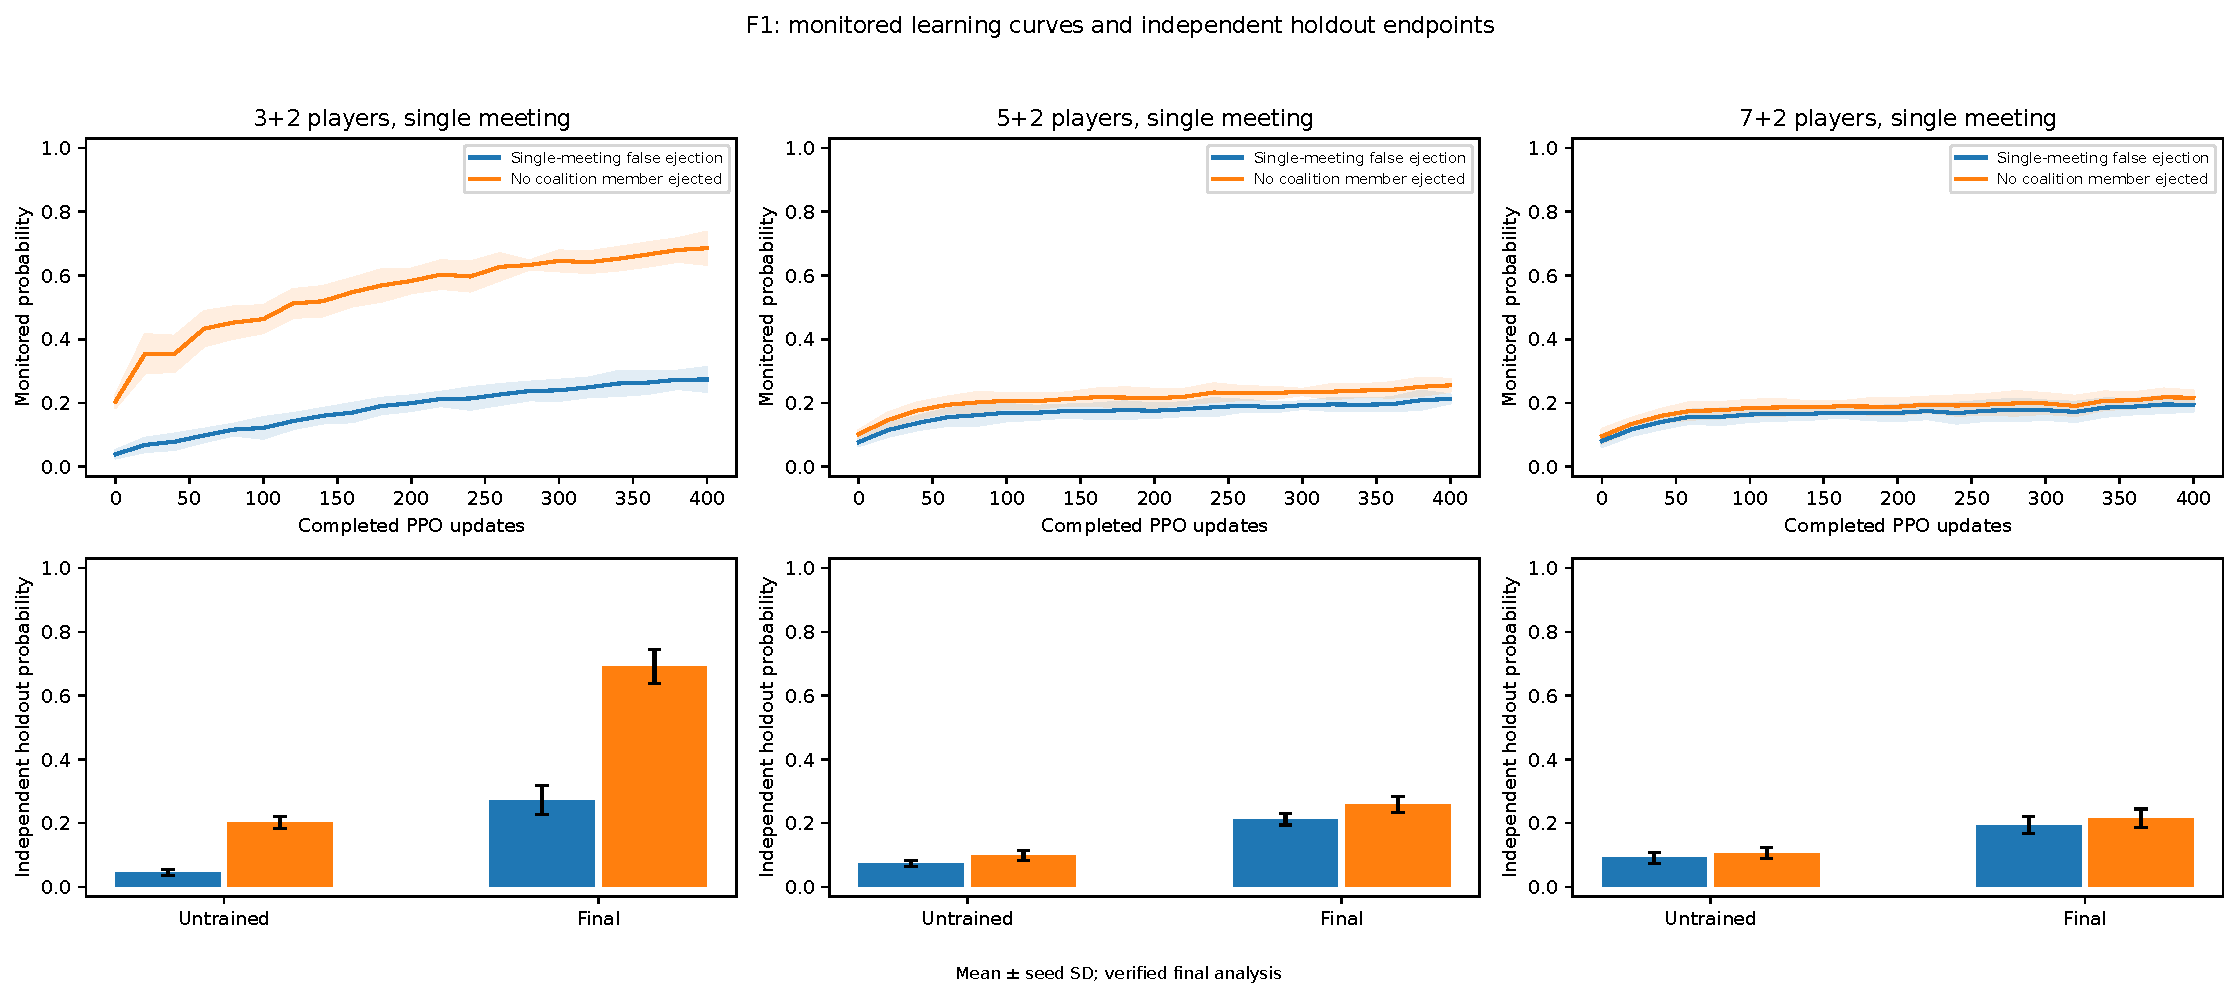
\includegraphics[width=1\linewidth,height=0.65\textheight]{figures/final/f1_learning_and_holdout.pdf}
\caption{Figure 1. Meeting-only learning at all three populations.
Curves use monitored evaluations; initial and final points use an
independent holdout stream. Lines and error bars describe ten-seed
variability, not independent episode replicates.}\label{fig:1}
\end{figure}

\FloatBarrier

\begin{table}[htbp]
\centering
\caption{Table 2. Independent holdout outcomes, mean ± sample SD across ten
seeds. Aligned votes exclude shared abstention; creator survival is
incident-gated. False claims count the FALSE label, separately from
contradictions and no-information.}\label{tab:2}
\begin{tabular}{@{}lrrr@{}}
\toprule\noalign{}
Players & Outcome & Untrained & Final \\
\midrule\noalign{}

3+2 & False ejection & 0.045 ± 0.011 & 0.271 ± 0.046 \\
3+2 & Aligned votes & 0.126 ± 0.023 & 0.613 ± 0.062 \\
3+2 & False claims & 0.429 ± 0.017 & 0.328 ± 0.074 \\
3+2 & Creator survives & 0.457 ± 0.024 & 0.789 ± 0.036 \\
5+2 & False ejection & 0.073 ± 0.008 & 0.212 ± 0.018 \\
5+2 & Aligned votes & 0.108 ± 0.023 & 0.316 ± 0.058 \\
5+2 & False claims & 0.423 ± 0.012 & 0.349 ± 0.046 \\
5+2 & Creator survives & 0.310 ± 0.020 & 0.438 ± 0.023 \\
7+2 & False ejection & 0.091 ± 0.017 & 0.194 ± 0.027 \\
7+2 & Aligned votes & 0.092 ± 0.016 & 0.244 ± 0.041 \\
7+2 & False claims & 0.420 ± 0.011 & 0.385 ± 0.048 \\
7+2 & Creator survives & 0.272 ± 0.018 & 0.366 ± 0.022 \\
\bottomrule\noalign{}
\end{tabular}
\end{table}

False ejection rises from 0.045 to 0.271 at 3+2, 0.073 to 0.2125 at 5+2,
and 0.091 to 0.194 at 7+2. All three specified final-minus-initial
false-ejection contrasts have Holm-adjusted \(p=0.0117\) within the
six-test F1 family. Aligned voting and creator survival also increase
descriptively, while the directly false-claim fraction falls at all
sizes. These joint changes show that harmful coordination need not
involve more explicitly false statements; they do not isolate
communication as a causal driver.

\FloatBarrier

\subsection{F2: testimony rules against scripted
coalitions}\label{f2-testimony-rules-against-scripted-coalitions}

\begin{figure}
\centering
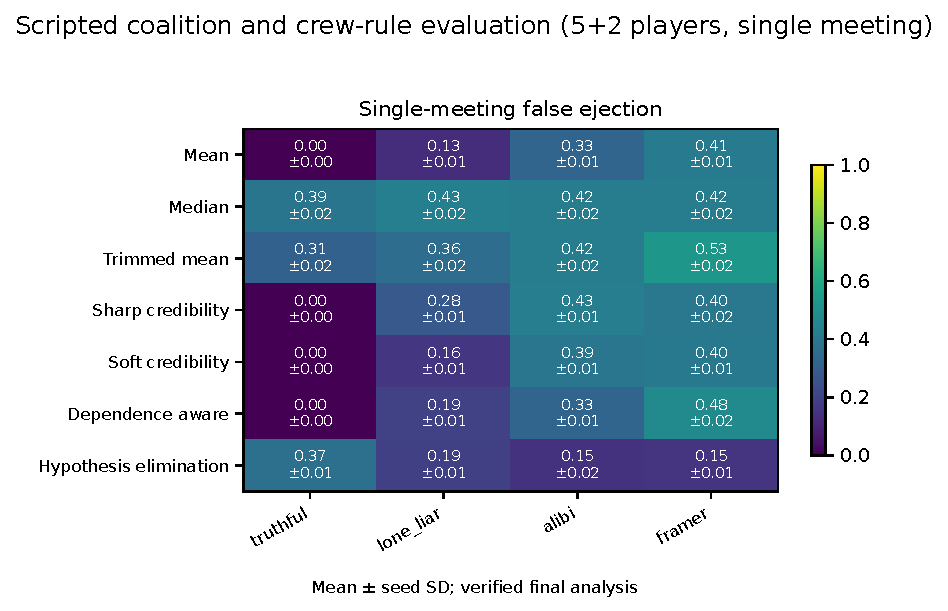
\includegraphics[width=1\linewidth,height=0.65\textheight]{figures/final/f2_tenseed_crew5_rules.pdf}
\caption{Figure 2. Seven rules against scripted testimony at 5+2, using
ten replicates and 1,000 episodes per cell. False-ejection and
creator-ejection outcomes answer different questions; the complete
three-population values accompany the analysis.}\label{fig:2}
\end{figure}

\FloatBarrier

\begin{table}[htbp]
\centering
\caption{Table 3. False-ejection probability. Entries are ten-replicate means;
complete sample SDs and seed identities are in the accompanying
machine-readable tables. Truthful concerns supported claim contents,
while coalition voting and information selection remain adversarial.}\label{tab:3}
\begin{tabular}{@{}
  >{\raggedright\arraybackslash}p{(\linewidth - 14\tabcolsep) * \real{0.1200}}
  >{\raggedleft\arraybackslash}p{(\linewidth - 14\tabcolsep) * \real{0.1250}}
  >{\raggedleft\arraybackslash}p{(\linewidth - 14\tabcolsep) * \real{0.1300}}
  >{\raggedleft\arraybackslash}p{(\linewidth - 14\tabcolsep) * \real{0.1250}}
  >{\raggedleft\arraybackslash}p{(\linewidth - 14\tabcolsep) * \real{0.1250}}
  >{\raggedleft\arraybackslash}p{(\linewidth - 14\tabcolsep) * \real{0.1250}}
  >{\raggedleft\arraybackslash}p{(\linewidth - 14\tabcolsep) * \real{0.1250}}
  >{\raggedleft\arraybackslash}p{(\linewidth - 14\tabcolsep) * \real{0.1250}}@{}}
\toprule\noalign{}
\begin{minipage}[b]{\linewidth}\raggedright
Players / script
\end{minipage} & \begin{minipage}[b]{\linewidth}\raggedleft
Mean
\end{minipage} & \begin{minipage}[b]{\linewidth}\raggedleft
Median
\end{minipage} & \begin{minipage}[b]{\linewidth}\raggedleft
Trim.
\end{minipage} & \begin{minipage}[b]{\linewidth}\raggedleft
Soft
\end{minipage} & \begin{minipage}[b]{\linewidth}\raggedleft
Sharp
\end{minipage} & \begin{minipage}[b]{\linewidth}\raggedleft
Dep.
\end{minipage} & \begin{minipage}[b]{\linewidth}\raggedleft
Hyp.
\end{minipage} \\
\midrule\noalign{}

3+2 Truthful & 0.000 & 0.137 & 0.137 & 0.000 & 0.000 & 0.000 & 0.245 \\
3+2 Lone & 0.328 & 0.245 & 0.245 & 0.178 & 0.204 & 0.210 & 0.412 \\
3+2 Alibi & 0.512 & 0.439 & 0.439 & 0.524 & 0.504 & 0.451 & 0.482 \\
3+2 Framer & 0.542 & 0.532 & 0.532 & 0.535 & 0.519 & 0.535 & 0.352 \\
5+2 Truthful & 0.000 & 0.389 & 0.312 & 0.000 & 0.000 & 0.000 & 0.370 \\
5+2 Lone & 0.131 & 0.430 & 0.359 & 0.159 & 0.278 & 0.194 & 0.191 \\
5+2 Alibi & 0.327 & 0.422 & 0.419 & 0.392 & 0.428 & 0.326 & 0.147 \\
5+2 Framer & 0.411 & 0.423 & 0.531 & 0.403 & 0.400 & 0.479 & 0.154 \\
7+2 Truthful & 0.000 & 0.504 & 0.380 & 0.000 & 0.000 & 0.000 & 0.393 \\
7+2 Lone & 0.100 & 0.553 & 0.417 & 0.151 & 0.300 & 0.178 & 0.070 \\
7+2 Alibi & 0.212 & 0.557 & 0.486 & 0.378 & 0.451 & 0.340 & 0.065 \\
7+2 Framer & 0.260 & 0.522 & 0.535 & 0.255 & 0.314 & 0.355 & 0.088 \\
\bottomrule\noalign{}
\end{tabular}
\end{table}

\FloatBarrier

\begin{table}[htbp]
\centering
\caption{Table 4. Incident-creator ejection probability. Entries are
ten-replicate means; complete sample SDs and seed identities are in the
accompanying machine-readable tables. Truthful concerns supported claim
contents, while coalition voting and information selection remain
adversarial.}\label{tab:4}
\begin{tabular}{@{}
  >{\raggedright\arraybackslash}p{(\linewidth - 14\tabcolsep) * \real{0.1200}}
  >{\raggedleft\arraybackslash}p{(\linewidth - 14\tabcolsep) * \real{0.1250}}
  >{\raggedleft\arraybackslash}p{(\linewidth - 14\tabcolsep) * \real{0.1300}}
  >{\raggedleft\arraybackslash}p{(\linewidth - 14\tabcolsep) * \real{0.1250}}
  >{\raggedleft\arraybackslash}p{(\linewidth - 14\tabcolsep) * \real{0.1250}}
  >{\raggedleft\arraybackslash}p{(\linewidth - 14\tabcolsep) * \real{0.1250}}
  >{\raggedleft\arraybackslash}p{(\linewidth - 14\tabcolsep) * \real{0.1250}}
  >{\raggedleft\arraybackslash}p{(\linewidth - 14\tabcolsep) * \real{0.1250}}@{}}
\toprule\noalign{}
\begin{minipage}[b]{\linewidth}\raggedright
Players / script
\end{minipage} & \begin{minipage}[b]{\linewidth}\raggedleft
Mean
\end{minipage} & \begin{minipage}[b]{\linewidth}\raggedleft
Median
\end{minipage} & \begin{minipage}[b]{\linewidth}\raggedleft
Trim.
\end{minipage} & \begin{minipage}[b]{\linewidth}\raggedleft
Soft
\end{minipage} & \begin{minipage}[b]{\linewidth}\raggedleft
Sharp
\end{minipage} & \begin{minipage}[b]{\linewidth}\raggedleft
Dep.
\end{minipage} & \begin{minipage}[b]{\linewidth}\raggedleft
Hyp.
\end{minipage} \\
\midrule\noalign{}

3+2 Truthful & 0.052 & 0.036 & 0.036 & 0.052 & 0.052 & 0.052 & 0.019 \\
3+2 Lone & 0.178 & 0.165 & 0.165 & 0.171 & 0.155 & 0.142 & 0.158 \\
3+2 Alibi & 0.000 & 0.000 & 0.000 & 0.000 & 0.000 & 0.000 & 0.000 \\
3+2 Framer & 0.000 & 0.000 & 0.000 & 0.000 & 0.000 & 0.000 & 0.000 \\
5+2 Truthful & 0.901 & 0.415 & 0.521 & 0.901 & 0.901 & 0.901 & 0.475 \\
5+2 Lone & 0.661 & 0.358 & 0.461 & 0.563 & 0.407 & 0.490 & 0.555 \\
5+2 Alibi & 0.354 & 0.351 & 0.310 & 0.221 & 0.213 & 0.362 & 0.360 \\
5+2 Framer & 0.380 & 0.353 & 0.237 & 0.409 & 0.410 & 0.328 & 0.386 \\
7+2 Truthful & 0.930 & 0.314 & 0.492 & 0.930 & 0.930 & 0.930 & 0.495 \\
7+2 Lone & 0.779 & 0.279 & 0.453 & 0.657 & 0.485 & 0.606 & 0.834 \\
7+2 Alibi & 0.560 & 0.277 & 0.344 & 0.332 & 0.298 & 0.457 & 0.604 \\
7+2 Framer & 0.590 & 0.279 & 0.299 & 0.612 & 0.560 & 0.532 & 0.592 \\
\bottomrule\noalign{}
\end{tabular}
\end{table}

The repaired hypothesis rule has a substantial truthful-testimony cost:
false ejection is 0.2447, 0.3700, and 0.3926 at 3+2, 5+2, and 7+2, while
mean and soft credibility have zero observed errors in these cells. At
5+2, hypothesis scoring improves on the mean under alibi (0.1469 versus
0.3273) and framer (0.1542 versus 0.4106), but worsens lone-liar error
(0.1907 versus 0.1311). Median and trimming can discard useful sparse
testimony; their robustness to scalar contamination does not guarantee
accurate votes here.

The F2 condition and rule families contain 63 and 36 contrasts. Their
adjusted tests do not reject at 0.05 under the retained ten-seed
resolution. Large descriptive differences should therefore be read with
their reported between-replicate variability, not promoted into
unreported familywise conclusions.

A bounded replay examined ten truthful-testimony false ejections from
one 5+2 seed. The true coalition retained positive weight in all 40
honest pre-vote views, and the actual timelines satisfied the emitted
constraints. Equal membership/creator scores could select an innocent
through deterministic index tie breaking; in another case every honest
voter skipped and coalition ballots alone decided the ejection. This
establishes concrete failure routes, not their prevalence across the
entire F2 distribution. Hard feasibility does not guarantee calibrated
scores or accurate decisions.

\subsubsection{Credibility weights and score
interventions}\label{credibility-weights-and-score-interventions}

We conducted a separate mechanism replication using the repaired frozen
implementation: ten evaluation replicates with 500 meetings each for
every combination of three initial crew sizes, four scripted conditions,
three aggregation rules, and three variants (540,000 meetings). Tables 5
and 6 report means and sample SDs across replicates. These new
measurements supersede the former single-seed mechanism diagnostic; they
use a separate matched-evidence stream from the full F2 rule sweep
above. Within each size, condition, and replicate, all nine rule/variant
cells share the same exogenous evidence and episode identities. The
interventions govern crew responses and votes, so subsequent public
responses may differ; they do not hold the full transcript fixed.

\FloatBarrier

\begin{table}[htbp]
\centering
\caption{Table 5. New pre-ejection soft-credibility diagnostic (mean ± SD across
ten replicates of 500 meetings each). C/H denote coalition/honest
speakers. Coalition weight is total normalized speaker weight;
parentheses give its uniform share. All honest voters are included,
including a voter subsequently ejected.}\label{tab:5}
\begin{tabular}{@{}
  >{\raggedright\arraybackslash}p{(\linewidth - 10\tabcolsep) * \real{0.1667}}
  >{\raggedleft\arraybackslash}p{(\linewidth - 10\tabcolsep) * \real{0.1667}}
  >{\raggedleft\arraybackslash}p{(\linewidth - 10\tabcolsep) * \real{0.1667}}
  >{\raggedleft\arraybackslash}p{(\linewidth - 10\tabcolsep) * \real{0.1667}}
  >{\raggedleft\arraybackslash}p{(\linewidth - 10\tabcolsep) * \real{0.1667}}
  >{\raggedleft\arraybackslash}p{(\linewidth - 10\tabcolsep) * \real{0.1667}}@{}}
\toprule\noalign{}
\begin{minipage}[b]{\linewidth}\raggedright
Game, condition
\end{minipage} & \begin{minipage}[b]{\linewidth}\raggedleft
Credibility C
\end{minipage} & \begin{minipage}[b]{\linewidth}\raggedleft
Credibility H
\end{minipage} & \begin{minipage}[b]{\linewidth}\raggedleft
Coalition weight (uniform)
\end{minipage} & \begin{minipage}[b]{\linewidth}\raggedleft
Coalition caught
\end{minipage} & \begin{minipage}[b]{\linewidth}\raggedleft
Top pick differs
\end{minipage} \\
\midrule\noalign{}

3+2, Truthful & 3.000 ± 0.000 & 3.000 ± 0.000 & 0.5000 ± 0.0000 (0.5000)
& 0.0000 ± 0.0000 & 0.0000 ± 0.0000 \\
3+2, Lone liar & 1.581 ± 0.037 & 2.982 ± 0.006 & 0.4225 ± 0.0022
(0.5000) & 0.4649 ± 0.0129 & 0.1264 ± 0.0076 \\
3+2, Alibi & 0.164 ± 0.075 & 2.960 ± 0.008 & 0.2630 ± 0.0059 (0.5000) &
0.5583 ± 0.0147 & 0.1674 ± 0.0161 \\
3+2, Framer & -1.547 ± 0.052 & 2.593 ± 0.040 & 0.1479 ± 0.0041 (0.5000)
& 0.7787 ± 0.0080 & 0.0029 ± 0.0014 \\
5+2, Truthful & 5.000 ± 0.000 & 5.000 ± 0.000 & 0.3333 ± 0.0000 (0.3333)
& 0.0000 ± 0.0000 & 0.0000 ± 0.0000 \\
5+2, Lone liar & 2.836 ± 0.054 & 4.987 ± 0.003 & 0.2606 ± 0.0017
(0.3333) & 0.5353 ± 0.0138 & 0.0319 ± 0.0054 \\
5+2, Alibi & 0.778 ± 0.078 & 4.970 ± 0.004 & 0.1425 ± 0.0030 (0.3333) &
0.6317 ± 0.0093 & 0.0769 ± 0.0085 \\
5+2, Framer & -0.335 ± 0.081 & 4.476 ± 0.025 & 0.1062 ± 0.0035 (0.3333)
& 0.6921 ± 0.0125 & 0.0085 ± 0.0021 \\
7+2, Truthful & 7.000 ± 0.000 & 7.000 ± 0.000 & 0.2500 ± 0.0000 (0.2500)
& 0.0000 ± 0.0000 & 0.0000 ± 0.0000 \\
7+2, Lone liar & 4.068 ± 0.036 & 6.989 ± 0.002 & 0.1863 ± 0.0010
(0.2500) & 0.5819 ± 0.0064 & 0.0174 ± 0.0036 \\
7+2, Alibi & 1.520 ± 0.124 & 6.973 ± 0.003 & 0.0976 ± 0.0027 (0.2500) &
0.6535 ± 0.0104 & 0.0672 ± 0.0069 \\
7+2, Framer & 0.361 ± 0.057 & 6.402 ± 0.013 & 0.0630 ± 0.0018 (0.2500) &
0.6830 ± 0.0080 & 0.0086 ± 0.0032 \\
\bottomrule\noalign{}
\end{tabular}
\end{table}

``Coalition caught'' is the fraction of honest voter decisions that
privately refute at least one coalition claim. ``Top pick differs''
compares mean and soft credibility on the same soft-baseline record,
restricted to eligible candidates. Credibility scores include refutation
and self-contradiction penalties as well as pairwise compatibility. One
crew member is removed by the incident before testimony: initial 3+2,
5+2, and 7+2 games have 2+2, 4+2, and 6+2 reporters. Appendix A counts
actual reporters, so 3+2 is outside its strict-minority condition
\(m<n\).

Under truthful testimony, all speakers receive the same credibility
score and the normalized weights are uniform; no same-record
mean-versus-soft top-pick differences were observed. All truthful cells
have zero observed false ejections, but this does not imply reliable
identification at every size. In truthful 3+2 baseline meetings, the
no-ejection rate is 0.9496 ± 0.0094 and the creator-ejection rate is
0.0504 ± 0.0094. At truthful 5+2 and 7+2 every meeting ejects a
coalition member, and creator-ejection rates are 0.9030 ± 0.0116 and
0.9204 ± 0.0113; remaining ejections select the partner.

For every attacked condition, the coalition's average normalized weight
is below its uniform share. In the coordinated alibi, the averages are
0.2630, 0.1425, and 0.0976 at initial 3+2, 5+2, and 7+2. Below-uniform
averages alone do not exclude individual episodes of weight capture. A
further audit of all 240,000 retained honest voter records found no
coalition weight above its uniform share at numerical tolerance
\(10^{-12}\). This is a descriptive result for these scripted records,
not a general immunity claim. All speakers supplied informative claims
in this experiment.

We tested two variants of each aggregation rule. ``Alibi off'' removes
testimony-based alibi credit, including the positive WAS\_WITH subject
credit controlled by the same coefficient. ``Catch outside'' places the
caught-lying suspicion penalty in the voter's own evidence instead of
within the speaker's aggregated row. In the baseline credibility
implementation, down-weighting a caught liar also reduces the
self-incriminating penalty contained in that row.

\FloatBarrier

\begin{longtable}[]{@{}
  >{\raggedright\arraybackslash}p{(\linewidth - 8\tabcolsep) * \real{0.2000}}
  >{\raggedright\arraybackslash}p{(\linewidth - 8\tabcolsep) * \real{0.2000}}
  >{\raggedleft\arraybackslash}p{(\linewidth - 8\tabcolsep) * \real{0.2000}}
  >{\raggedleft\arraybackslash}p{(\linewidth - 8\tabcolsep) * \real{0.2000}}
  >{\raggedleft\arraybackslash}p{(\linewidth - 8\tabcolsep) * \real{0.2000}}@{}}
\caption{Table 6. New false-ejection rates across all scripted
conditions, rules and variants (mean ± SD across ten replicates of 500
meetings per cell). Soft and sharp denote credibility rules. Evidence is
matched within each size/condition/replicate; responses and votes are
regenerated. Differences are descriptive.}\label{tab:6}\tabularnewline
\toprule\noalign{}
\begin{minipage}[b]{\linewidth}\raggedright
Game, condition
\end{minipage} & \begin{minipage}[b]{\linewidth}\raggedright
Rule
\end{minipage} & \begin{minipage}[b]{\linewidth}\raggedleft
Baseline
\end{minipage} & \begin{minipage}[b]{\linewidth}\raggedleft
Alibi off
\end{minipage} & \begin{minipage}[b]{\linewidth}\raggedleft
Catch outside
\end{minipage} \\
\midrule\noalign{}
\endfirsthead
\toprule\noalign{}
\begin{minipage}[b]{\linewidth}\raggedright
Game, condition
\end{minipage} & \begin{minipage}[b]{\linewidth}\raggedright
Rule
\end{minipage} & \begin{minipage}[b]{\linewidth}\raggedleft
Baseline
\end{minipage} & \begin{minipage}[b]{\linewidth}\raggedleft
Alibi off
\end{minipage} & \begin{minipage}[b]{\linewidth}\raggedleft
Catch outside
\end{minipage} \\
\midrule\noalign{}
\endhead
\bottomrule\noalign{}
\endlastfoot
3+2, Truthful & Mean & 0.0000 ± 0.0000 & 0.0000 ± 0.0000 & 0.0000 ±
0.0000 \\
3+2, Truthful & Soft & 0.0000 ± 0.0000 & 0.0000 ± 0.0000 & 0.0000 ±
0.0000 \\
3+2, Truthful & Sharp & 0.0000 ± 0.0000 & 0.0000 ± 0.0000 & 0.0000 ±
0.0000 \\
3+2, Lone liar & Mean & 0.3290 ± 0.0179 & 0.3662 ± 0.0184 & 0.3290 ±
0.0179 \\
3+2, Lone liar & Soft & 0.1734 ± 0.0205 & 0.2106 ± 0.0237 & 0.3274 ±
0.0178 \\
3+2, Lone liar & Sharp & 0.2010 ± 0.0230 & 0.2188 ± 0.0277 & 0.3230 ±
0.0175 \\
3+2, Alibi & Mean & 0.5176 ± 0.0249 & 0.4030 ± 0.0219 & 0.5180 ±
0.0250 \\
3+2, Alibi & Soft & 0.5288 ± 0.0238 & 0.3728 ± 0.0193 & 0.5046 ±
0.0223 \\
3+2, Alibi & Sharp & 0.5144 ± 0.0252 & 0.4406 ± 0.0222 & 0.4528 ±
0.0201 \\
3+2, Framer & Mean & 0.5354 ± 0.0195 & 0.5370 ± 0.0200 & 0.5354 ±
0.0195 \\
3+2, Framer & Soft & 0.5294 ± 0.0200 & 0.5306 ± 0.0198 & 0.5294 ±
0.0200 \\
3+2, Framer & Sharp & 0.5124 ± 0.0202 & 0.5172 ± 0.0209 & 0.5110 ±
0.0204 \\
5+2, Truthful & Mean & 0.0000 ± 0.0000 & 0.0000 ± 0.0000 & 0.0000 ±
0.0000 \\
5+2, Truthful & Soft & 0.0000 ± 0.0000 & 0.0000 ± 0.0000 & 0.0000 ±
0.0000 \\
5+2, Truthful & Sharp & 0.0000 ± 0.0000 & 0.0000 ± 0.0000 & 0.0000 ±
0.0000 \\
5+2, Lone liar & Mean & 0.1326 ± 0.0181 & 0.1876 ± 0.0171 & 0.1326 ±
0.0181 \\
5+2, Lone liar & Soft & 0.1598 ± 0.0184 & 0.2064 ± 0.0199 & 0.1316 ±
0.0189 \\
5+2, Lone liar & Sharp & 0.2792 ± 0.0187 & 0.3244 ± 0.0154 & 0.1316 ±
0.0189 \\
5+2, Alibi & Mean & 0.3122 ± 0.0198 & 0.2312 ± 0.0224 & 0.3122 ±
0.0198 \\
5+2, Alibi & Soft & 0.3802 ± 0.0242 & 0.2310 ± 0.0215 & 0.2890 ±
0.0183 \\
5+2, Alibi & Sharp & 0.4198 ± 0.0282 & 0.3414 ± 0.0191 & 0.2676 ±
0.0210 \\
5+2, Framer & Mean & 0.4060 ± 0.0248 & 0.5244 ± 0.0236 & 0.4060 ±
0.0248 \\
5+2, Framer & Soft & 0.4014 ± 0.0275 & 0.4890 ± 0.0259 & 0.4010 ±
0.0276 \\
5+2, Framer & Sharp & 0.4054 ± 0.0214 & 0.4706 ± 0.0229 & 0.3790 ±
0.0261 \\
7+2, Truthful & Mean & 0.0000 ± 0.0000 & 0.0000 ± 0.0000 & 0.0000 ±
0.0000 \\
7+2, Truthful & Soft & 0.0000 ± 0.0000 & 0.0000 ± 0.0000 & 0.0000 ±
0.0000 \\
7+2, Truthful & Sharp & 0.0000 ± 0.0000 & 0.0000 ± 0.0000 & 0.0000 ±
0.0000 \\
7+2, Lone liar & Mean & 0.0908 ± 0.0179 & 0.1416 ± 0.0139 & 0.0908 ±
0.0179 \\
7+2, Lone liar & Soft & 0.1438 ± 0.0231 & 0.1834 ± 0.0169 & 0.0902 ±
0.0179 \\
7+2, Lone liar & Sharp & 0.3012 ± 0.0237 & 0.3672 ± 0.0205 & 0.0902 ±
0.0179 \\
7+2, Alibi & Mean & 0.2080 ± 0.0190 & 0.1632 ± 0.0191 & 0.2080 ±
0.0190 \\
7+2, Alibi & Soft & 0.3666 ± 0.0250 & 0.2090 ± 0.0157 & 0.1916 ±
0.0193 \\
7+2, Alibi & Sharp & 0.4362 ± 0.0256 & 0.4012 ± 0.0254 & 0.1786 ±
0.0199 \\
7+2, Framer & Mean & 0.2654 ± 0.0176 & 0.4670 ± 0.0212 & 0.2654 ±
0.0176 \\
7+2, Framer & Soft & 0.2574 ± 0.0180 & 0.3906 ± 0.0212 & 0.2568 ±
0.0176 \\
7+2, Framer & Sharp & 0.3162 ± 0.0163 & 0.4192 ± 0.0231 & 0.2412 ±
0.0172 \\
\end{longtable}

Mean catch-outside false-ejection outcomes differ from baseline only in
two 3+2 alibi episodes (0.5176 versus 0.5180): replays locate a
\(2.22\times10^{-16}\) change in one candidate score that resolves a
floating-point argmax tie and changes the meeting outcome. Algebraic
equality therefore does not imply bitwise equality of decisions.

In the alibi condition, soft credibility exceeds the baseline mean's
false-ejection rate by paired differences of 0.0112 ± 0.0080, 0.0680 ±
0.0136, and 0.1586 ± 0.0112 at 3+2, 5+2, and 7+2. Moving the caught
penalty outside reduces soft alibi false ejections by 0.0242 ± 0.0066,
0.0912 ± 0.0150, and 0.1750 ± 0.0084 relative to its own baseline.
Removing alibi credit also lowers alibi false ejections for every tested
rule and size. These interventions support a role for alibi credit and
catch-penalty placement in the observed behavior, while allowing
responses and resulting testimony use to change.

The improvements are conditional on the attack and size. Removing alibi
credit raises lone-liar and framer false ejections; for soft credibility
under the framer the increases are 0.0876 ± 0.0143 at 5+2 and 0.1332 ±
0.0222 at 7+2. Moving the caught penalty outside raises the soft
lone-liar rate at 3+2 by 0.1540 ± 0.0188, although it reduces lone-liar
false ejections at the larger sizes. Soft framer rates change by at most
0.0006 under catch-outside. Sharper weighting also has no uniform
advantage: at 7+2 its baseline false-ejection rate exceeds the mean by
0.2104 ± 0.0139 for the lone liar, 0.2282 ± 0.0172 for alibi, and 0.0508
± 0.0124 for the framer.

False-ejection reductions can reflect abstention or tied votes rather
than more correct ejections. Under coordinated alibi at 3+2, every
tested rule/variant has creator-ejection rate zero and
coalition-favorable rate one; reducing false ejections only increases
no-ejection outcomes. Under the lone liar at 5+2, soft catch-outside
lowers false ejection from 0.1598 to 0.1316, but raises no-ejection from
0.0402 ± 0.0049 to 0.1100 ± 0.0105 and coalition-favorable outcomes from
0.2000 ± 0.0207 to 0.2416 ± 0.0257. Thus these measurements distinguish
testimony-based alibi support and catch-penalty placement from increased
coalition weight, without establishing a unique causal explanation or an
improvement under every objective.

\FloatBarrier

\subsection{F3: single-meeting crossplay depends on opponent and
population}\label{f3-single-meeting-crossplay-depends-on-opponent-and-population}

\begin{figure}
\centering
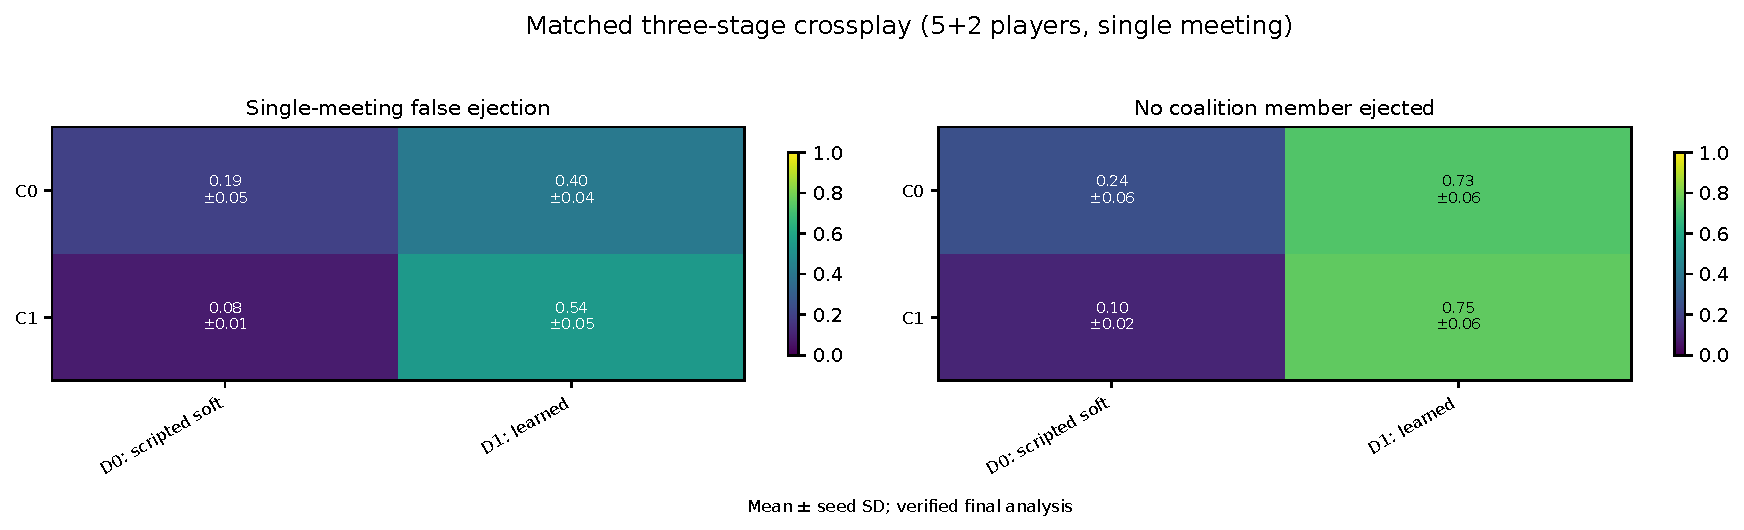
\includegraphics[width=1\linewidth,height=0.65\textheight]{figures/final/f3_tenseed_crew5_crossplay.pdf}
\caption{Figure 3. Spatial single-meeting crossplay at 5+2, including
false ejection, incident opportunity, and creator outcomes. Each cell
uses all ten seeds and 1,000 final games per seed.}\label{fig:3}
\end{figure}

\FloatBarrier

\begin{table}[htbp]
\centering
\caption{Table 7. Unconditional per-game probabilities, mean ± sample SD across
ten seeds. Creator ejection requires an incident. D0 is scripted; D1 and
C1 are fresh policies trained against their frozen predecessor.}\label{tab:7}
\begin{tabular}{@{}lrrrr@{}}
\toprule\noalign{}
Players & Pair & False ejection & Incident & Creator ejected \\
\midrule\noalign{}

3+2 & C0--D0 & 0.188 ± 0.045 & 0.986 ± 0.005 & 0.128 ± 0.049 \\
3+2 & C0--D1 & 0.463 ± 0.073 & 0.087 ± 0.140 & 0.016 ± 0.030 \\
3+2 & C1--D1 & 0.415 ± 0.089 & 0.302 ± 0.286 & 0.025 ± 0.034 \\
3+2 & C1--D0 & 0.068 ± 0.034 & 0.949 ± 0.089 & 0.341 ± 0.101 \\
5+2 & C0--D0 & 0.194 ± 0.051 & 0.963 ± 0.027 & 0.566 ± 0.054 \\
5+2 & C0--D1 & 0.403 ± 0.040 & 0.254 ± 0.178 & 0.051 ± 0.035 \\
5+2 & C1--D1 & 0.538 ± 0.053 & 0.788 ± 0.132 & 0.092 ± 0.024 \\
5+2 & C1--D0 & 0.076 ± 0.014 & 0.984 ± 0.003 & 0.686 ± 0.036 \\
7+2 & C0--D0 & 0.211 ± 0.022 & 0.943 ± 0.030 & 0.584 ± 0.039 \\
7+2 & C0--D1 & 0.475 ± 0.037 & 0.321 ± 0.216 & 0.036 ± 0.026 \\
7+2 & C1--D1 & 0.587 ± 0.040 & 0.754 ± 0.117 & 0.061 ± 0.019 \\
7+2 & C1--D0 & 0.083 ± 0.020 & 0.970 ± 0.010 & 0.710 ± 0.032 \\
\bottomrule\noalign{}
\end{tabular}
\end{table}

At 5+2, false ejection rises from 0.1940 for C0--D0 to 0.4031 for
C0--D1, then to 0.5385 for C1--D1. Against D0 the adapted coalition
achieves only 0.0759. The specified defender-effect contrast is C0--D0
minus C0--D1; it is negative at all three sizes (-0.2752, -0.2091,
-0.2638), with Holm-adjusted \(p=0.0176\). Thus the learned defender has
more innocent ejections against the same frozen coalition.

Coalition adaptation against D1 has different signs across populations.
At 3+2 the mean falls from 0.4635 to 0.4153, an effect of -0.0482 that
does not reject; at 5+2 and 7+2 the increases are 0.1354 and 0.1124.
Full paired intervals and adjusted tests are supplied alongside the
tables. The data do not support a universal increase from coalition
retraining.

C0 creates incidents in 0.986, 0.963, and 0.943 of games against D0,
versus 0.087, 0.254, and 0.321 against D1. Changing the defender also
changes movement, opportunities, and testimony. Conditional error is
therefore not an isolated reasoning comparison. Some 3+2 seeds have no
incidents against D1: their incident-conditional rates remain undefined,
while all unconditional summaries retain ten seeds. The formerly
reported rare-incident account does not describe this corrected
implementation; multiple repairs changed together, so their individual
causal contributions are not identified.

\FloatBarrier

\subsection{F4: coalition victory and whole-game harm can
diverge}\label{f4-coalition-victory-and-whole-game-harm-can-diverge}

\begin{figure}
\centering
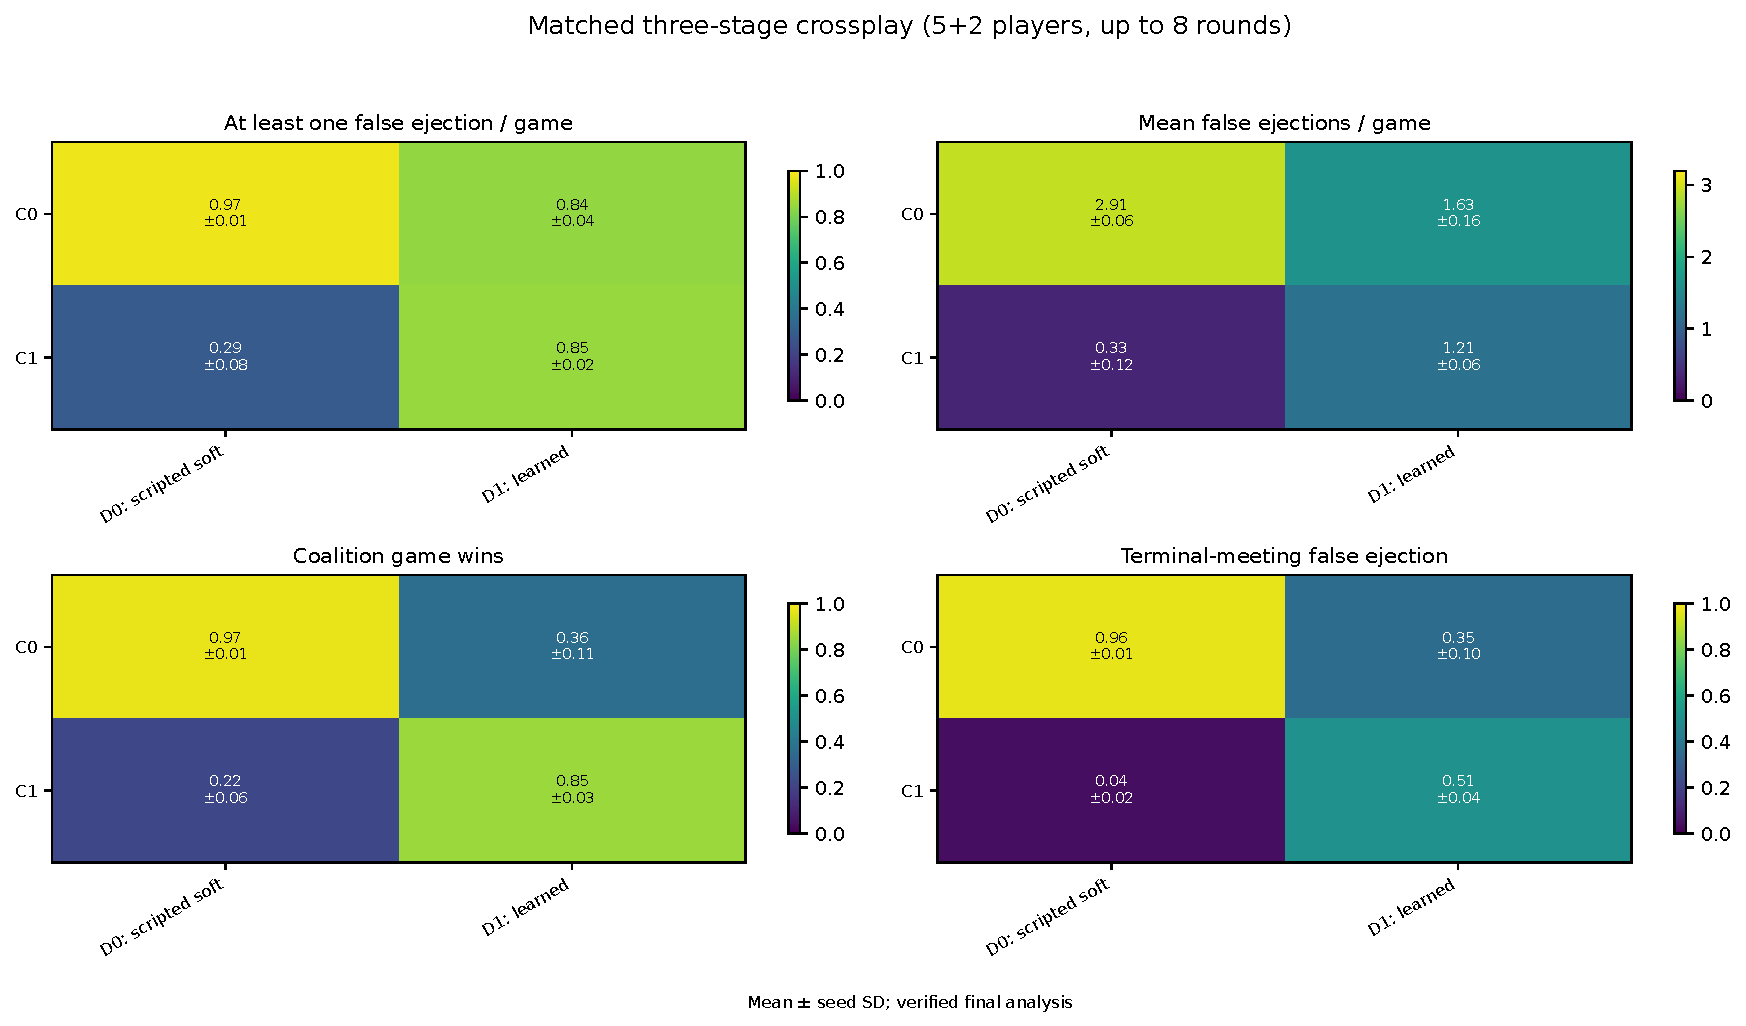
\includegraphics[width=1\linewidth,height=0.65\textheight]{figures/final/f4_tenseed_crew5_crossplay.pdf}
\caption{Figure 4. Multi-round crossplay at 5+2. Coalition victory, any
innocent ejection, mean innocent-ejection count, and terminal outcomes
are kept distinct. All ten seeds are included.}\label{fig:4}
\end{figure}

\FloatBarrier

\begin{table}[htbp]
\centering
\caption{Table 8. Whole-game outcomes, mean ± seed SD. Any innocent ejection
includes incident-free meetings; mean count is the number per game. It
is not a terminal-meeting probability.}\label{tab:8}
\begin{tabular}{@{}lrrrr@{}}
\toprule\noalign{}
Players & Pair & Coalition wins & Any innocent ejected & Mean count \\
\midrule\noalign{}

3+2 & C0--D0 & 0.997 ± 0.004 & 0.562 ± 0.312 & 0.626 ± 0.410 \\
3+2 & C0--D1 & 0.282 ± 0.255 & 0.286 ± 0.197 & 0.324 ± 0.251 \\
3+2 & C1--D1 & 0.941 ± 0.058 & 0.521 ± 0.076 & 0.539 ± 0.093 \\
3+2 & C1--D0 & 0.988 ± 0.021 & 0.088 ± 0.014 & 0.088 ± 0.014 \\
5+2 & C0--D0 & 0.967 ± 0.012 & 0.974 ± 0.012 & 2.906 ± 0.059 \\
5+2 & C0--D1 & 0.360 ± 0.106 & 0.839 ± 0.043 & 1.634 ± 0.163 \\
5+2 & C1--D1 & 0.851 ± 0.026 & 0.847 ± 0.019 & 1.209 ± 0.060 \\
5+2 & C1--D0 & 0.218 ± 0.058 & 0.289 ± 0.084 & 0.332 ± 0.117 \\
7+2 & C0--D0 & 0.963 ± 0.007 & 0.978 ± 0.009 & 4.862 ± 0.042 \\
7+2 & C0--D1 & 0.304 ± 0.026 & 0.947 ± 0.006 & 2.996 ± 0.095 \\
7+2 & C1--D1 & 0.814 ± 0.016 & 0.947 ± 0.005 & 1.989 ± 0.053 \\
7+2 & C1--D0 & 0.063 ± 0.026 & 0.409 ± 0.054 & 0.558 ± 0.112 \\
\bottomrule\noalign{}
\end{tabular}
\end{table}

At 5+2, coalition victory drops from 0.9670 for C0--D0 to 0.3603 for
C0--D1 and returns to 0.8514 for C1--D1. Yet any innocent ejection is
0.8392 and 0.8467 in the latter two pairings. The descriptive
coalition-adaptation effects are +0.4911 for victory and only +0.0075
for any false ejection; mean innocent-ejection count falls by 0.4249 per
game. At 7+2, victory rises by 0.5104 while mean count falls by 1.0066.
Shorter or differently terminated games can therefore combine more
coalition wins with fewer total innocent ejections. Reducing coalition
wins therefore coexists with frequent crew harm; victory alone is an
incomplete measure of defensive quality. Transfer again differs: C1--D0
wins only 0.2182 at 5+2 and 0.0630 at 7+2, but 0.9882 at 3+2.

None of the 27 F4 contrasts passes Holm correction at 0.05; the minimum
adjusted value is 0.0527, imposed by the ten-seed exact-test resolution.
The effect estimates remain relevant, but pointwise intervals do not
override that familywise result. Whole-game harm records replace the old
terminal-only interpretation.

\FloatBarrier

\subsection{Controls: information, defender budget, and reward
design}\label{controls-information-defender-budget-and-reward-design}

\FloatBarrier

\begin{table}[htbp]
\centering
\caption{Table 9. C0 information controls at 5+2, five seeds per condition.
Hidden partner changes information and communication together; it does
not prevent inference from observed events.}\label{tab:9}
\begin{tabular}{@{}lrrr@{}}
\toprule\noalign{}
Condition & Single FE & Multi any-FE & Multi win \\
\midrule\noalign{}

Default & 0.185 ± 0.071 & 0.973 ± 0.011 & 0.967 ± 0.010 \\
No channel & 0.218 ± 0.071 & 0.983 ± 0.003 & 0.977 ± 0.004 \\
Hidden partner & 0.208 ± 0.059 & 0.973 ± 0.007 & 0.962 ± 0.008 \\
Both removed & 0.252 ± 0.038 & 0.970 ± 0.014 & 0.963 ± 0.014 \\
\bottomrule\noalign{}
\end{tabular}
\end{table}

\begin{figure}
\centering
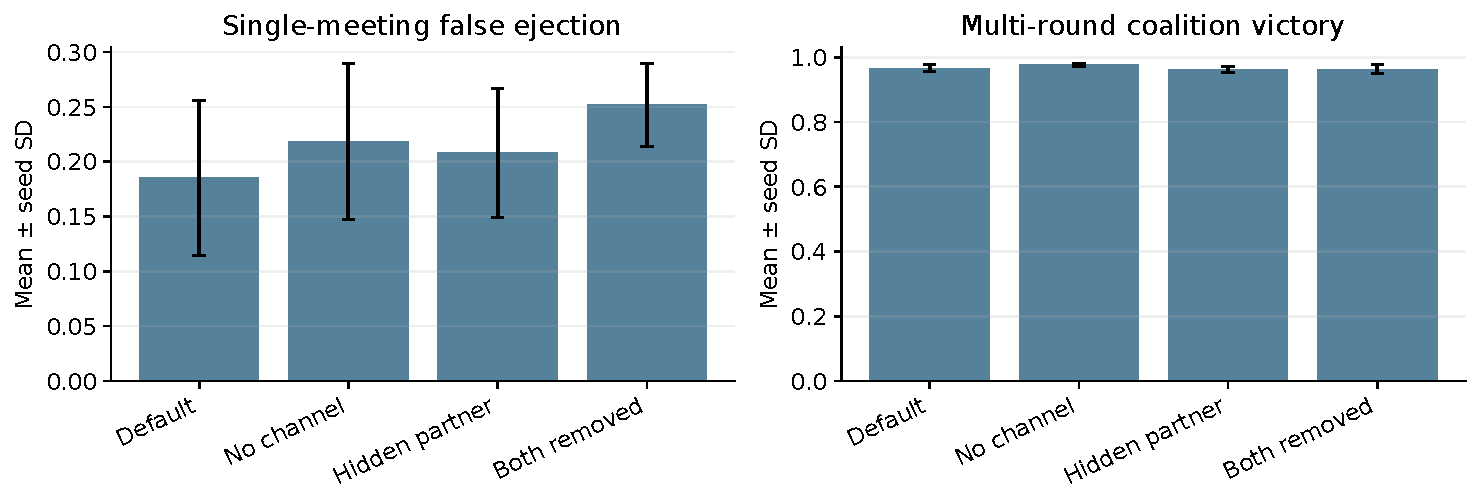
\includegraphics[width=1\linewidth,height=0.65\textheight]{figures/final/coordination_controls.pdf}
\caption{Figure 5. Information-control outcomes at 5+2, with sample SD
across five seeds. Error bars are descriptive and do not establish
equivalence.}\label{fig:5}
\end{figure}

Removing both aids gives single-meeting false ejection 0.2518 versus
0.1854 by default; this does not demonstrate that either aid is
necessary for harm. None of the nine planned outcome-ablation contrasts
rejects after Holm correction. The intervention does not remove shared
parameters, rewards, prearranged behavior, or all possible role
inference, and it tests only C0 rather than an entire response lineage.

\FloatBarrier

\begin{table}[htbp]
\centering
\caption{Table 10. Defender-budget controls at 5+2. Every row, including the
400-update reference, uses exactly seeds 0--4. C0 and C1 keep 400
updates.}\label{tab:10}
\begin{tabular}{@{}lrrr@{}}
\toprule\noalign{}
Outcome & Defender updates & C0--D1 & C1--D1 \\
\midrule\noalign{}

Single FE & 400 & 0.387 ± 0.040 & 0.525 ± 0.048 \\
Single FE & 800 & 0.439 ± 0.069 & 0.567 ± 0.055 \\
Single FE & 1600 & 0.382 ± 0.055 & 0.516 ± 0.039 \\
Multi any-FE & 400 & 0.840 ± 0.050 & 0.846 ± 0.012 \\
Multi any-FE & 800 & 0.745 ± 0.048 & 0.852 ± 0.034 \\
Multi win & 400 & 0.354 ± 0.115 & 0.854 ± 0.029 \\
Multi win & 800 & 0.165 ± 0.078 & 0.848 ± 0.029 \\
\bottomrule\noalign{}
\end{tabular}
\end{table}

\begin{figure}
\centering
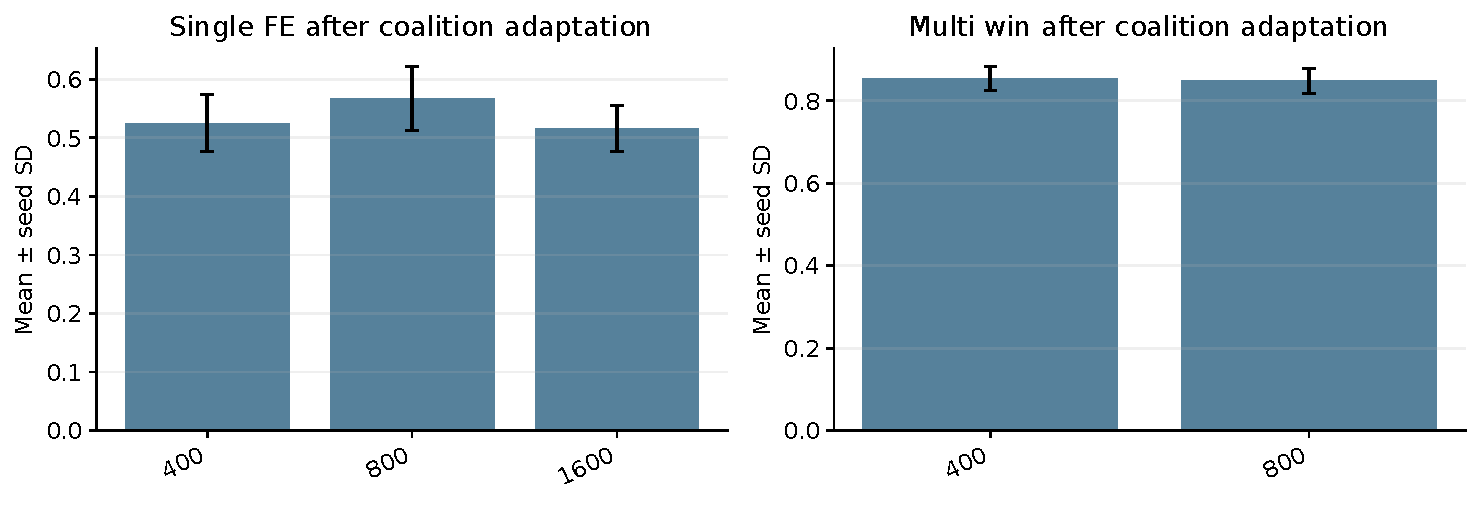
\includegraphics[width=1\linewidth,height=0.65\textheight]{figures/final/defender_budgets.pdf}
\caption{Figure 6. Matched-five-seed budget comparisons after coalition
adaptation. The reference is recomputed from those five seeds, not the
ten-seed headline estimate.}\label{fig:6}
\end{figure}

In single-meeting play, C1--D1 false ejection is 0.5252 at 400 defender
updates, 0.5672 at 800, and 0.5160 at 1,600 on the matched five seeds.
None of the eight budget contrasts rejects after Holm correction. These
finite budgets do not establish an optimal defender response, and the
five-seed minimum raw p-value is already above 0.05.

\FloatBarrier

\begin{table}[htbp]
\centering
\caption{Table 11. Reward controls, means ± SD across the same five seeds and
matched horizons: four generations for single-meeting, two for
multi-round. C-stage and D-stage means omit C0; matrix gain averages
M{[}g,g{]} minus M{[}g−1,g{]}.}\label{tab:11}
\begin{tabular}{@{}
  >{\raggedright\arraybackslash}p{(\linewidth - 8\tabcolsep) * \real{0.2000}}
  >{\raggedleft\arraybackslash}p{(\linewidth - 8\tabcolsep) * \real{0.2000}}
  >{\raggedleft\arraybackslash}p{(\linewidth - 8\tabcolsep) * \real{0.2000}}
  >{\raggedleft\arraybackslash}p{(\linewidth - 8\tabcolsep) * \real{0.2000}}
  >{\raggedleft\arraybackslash}p{(\linewidth - 8\tabcolsep) * \real{0.2000}}@{}}
\toprule\noalign{}
\begin{minipage}[b]{\linewidth}\raggedright
Outcome
\end{minipage} & \begin{minipage}[b]{\linewidth}\raggedleft
Reward
\end{minipage} & \begin{minipage}[b]{\linewidth}\raggedleft
C stages
\end{minipage} & \begin{minipage}[b]{\linewidth}\raggedleft
D stages
\end{minipage} & \begin{minipage}[b]{\linewidth}\raggedleft
Matrix gain
\end{minipage} \\
\midrule\noalign{}

Single FE & Default & 0.551 ± 0.040 & 0.267 ± 0.049 & 0.287 ± 0.075 \\
Single FE & Balanced & 0.548 ± 0.015 & 0.380 ± 0.018 & 0.164 ± 0.040 \\
Single FE & Meeting & 0.570 ± 0.051 & 0.347 ± 0.006 & 0.220 ± 0.049 \\
Multi any-FE & Survival & 0.854 ± 0.020 & 0.757 ± 0.060 & 0.101 ±
0.055 \\
Multi any-FE & Framing count & 0.888 ± 0.020 & 0.800 ± 0.029 & 0.090 ±
0.032 \\
Multi win & Survival & 0.810 ± 0.043 & 0.374 ± 0.076 & 0.440 ± 0.095 \\
Multi win & Framing count & 0.883 ± 0.014 & 0.554 ± 0.051 & 0.333 ±
0.060 \\
\bottomrule\noalign{}
\end{tabular}
\end{table}

\begin{figure}
\centering
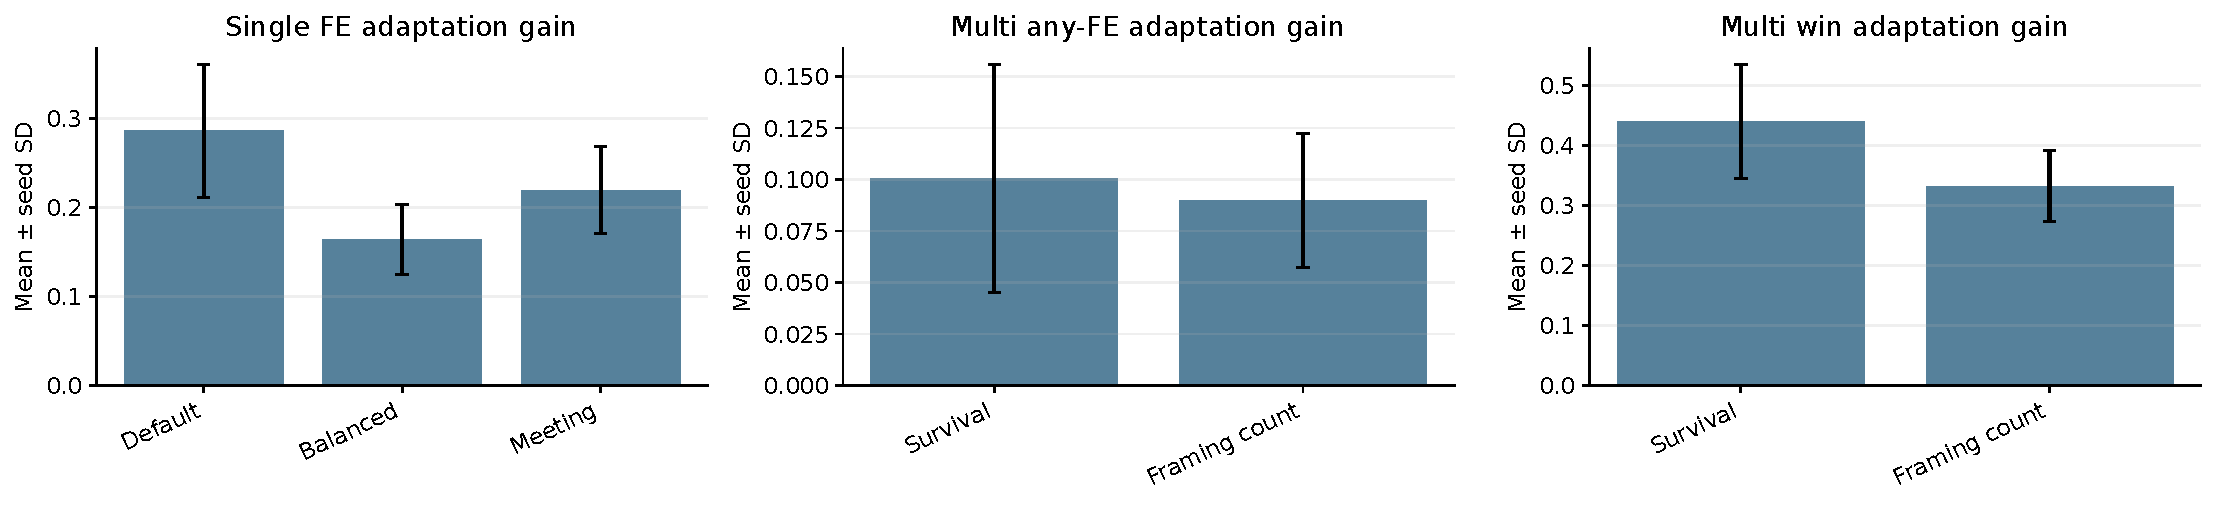
\includegraphics[width=1\linewidth,height=0.65\textheight]{figures/final/reward_controls.pdf}
\caption{Figure 7. Reward-control matrix adaptation gains on matched
seed cohorts and horizons. Panels report different outcomes, not a
common reward scale.}\label{fig:7}
\end{figure}

None of the 18 specified reward-control contrasts rejects after Holm
correction. The variants can alter outcome levels and response gains
descriptively; the evidence does not show that reward design is
irrelevant. Five seeds provide limited resolution, and the tested
objectives do not exhaust alternative incentives or learning algorithms.

\FloatBarrier

\subsection{F5: repeated gains over a finite response
sequence}\label{f5-repeated-gains-over-a-finite-response-sequence}

\begin{figure}
\centering
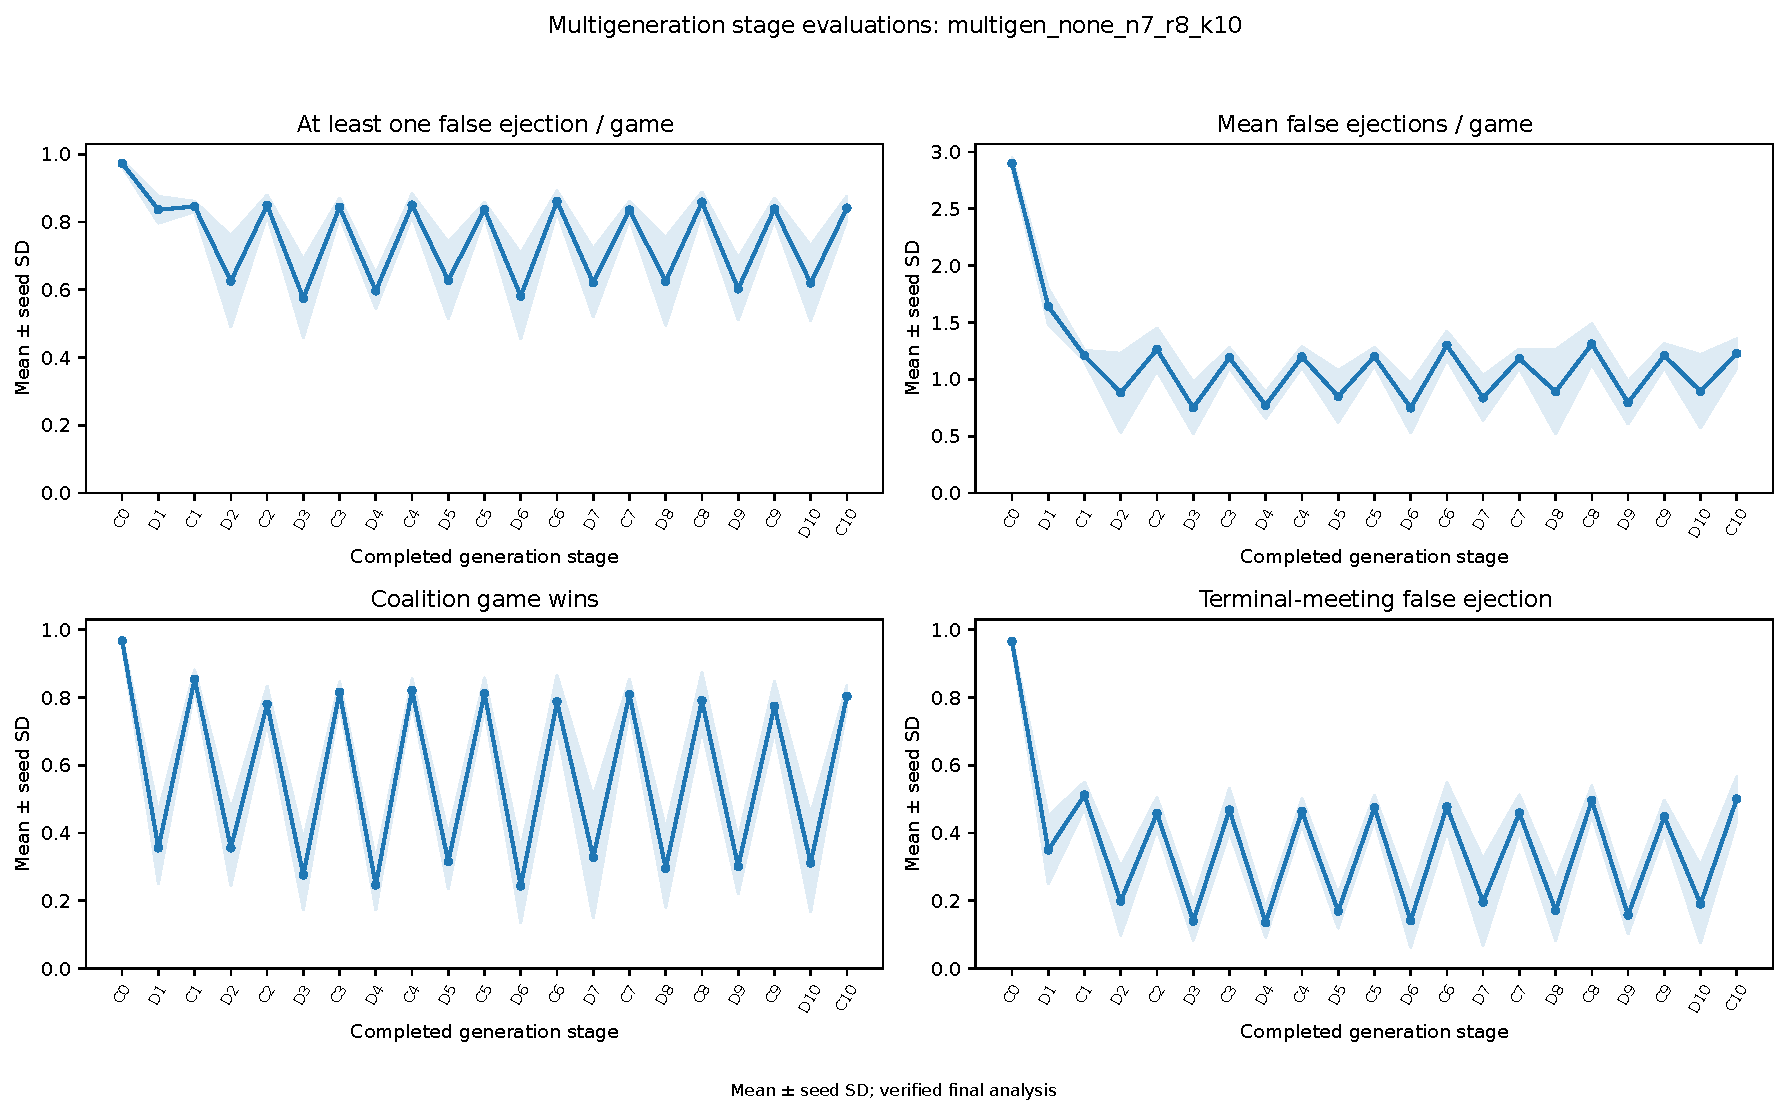
\includegraphics[width=1\linewidth,height=0.65\textheight]{figures/final/multigen_none_n7_r8_k10_stages.pdf}
\caption{Figure 8. The 5+2 multi-round sequence through ten generations,
ten seeds. C and D stages are independently initialized response
policies; monitored and holdout quantities remain
separate.}\label{fig:8}
\end{figure}

\FloatBarrier

\begin{table}[htbp]
\centering
\caption{Table 12. Finite-horizon response summaries. Single-meeting uses false
ejection; multi-round uses coalition victory. Stage means omit C0.
Matrix gains use final crossplay, not differences between monitored
curves.}\label{tab:12}
\begin{tabular}{@{}lrrrr@{}}
\toprule\noalign{}
Setting & Seeds & C stages & D stages & Matrix gain \\
\midrule\noalign{}

3+2 multi & 10 & 0.918 ± 0.021 & 0.341 ± 0.059 & 0.576 ± 0.050 \\
5+2 single & 10 & 0.557 ± 0.016 & 0.257 ± 0.023 & 0.300 ± 0.032 \\
5+2 multi & 10 & 0.804 ± 0.025 & 0.303 ± 0.035 & 0.501 ± 0.050 \\
7+2 multi & 5 & 0.752 ± 0.048 & 0.330 ± 0.044 & 0.418 ± 0.088 \\
\bottomrule\noalign{}
\end{tabular}
\end{table}

\begin{figure}
\centering
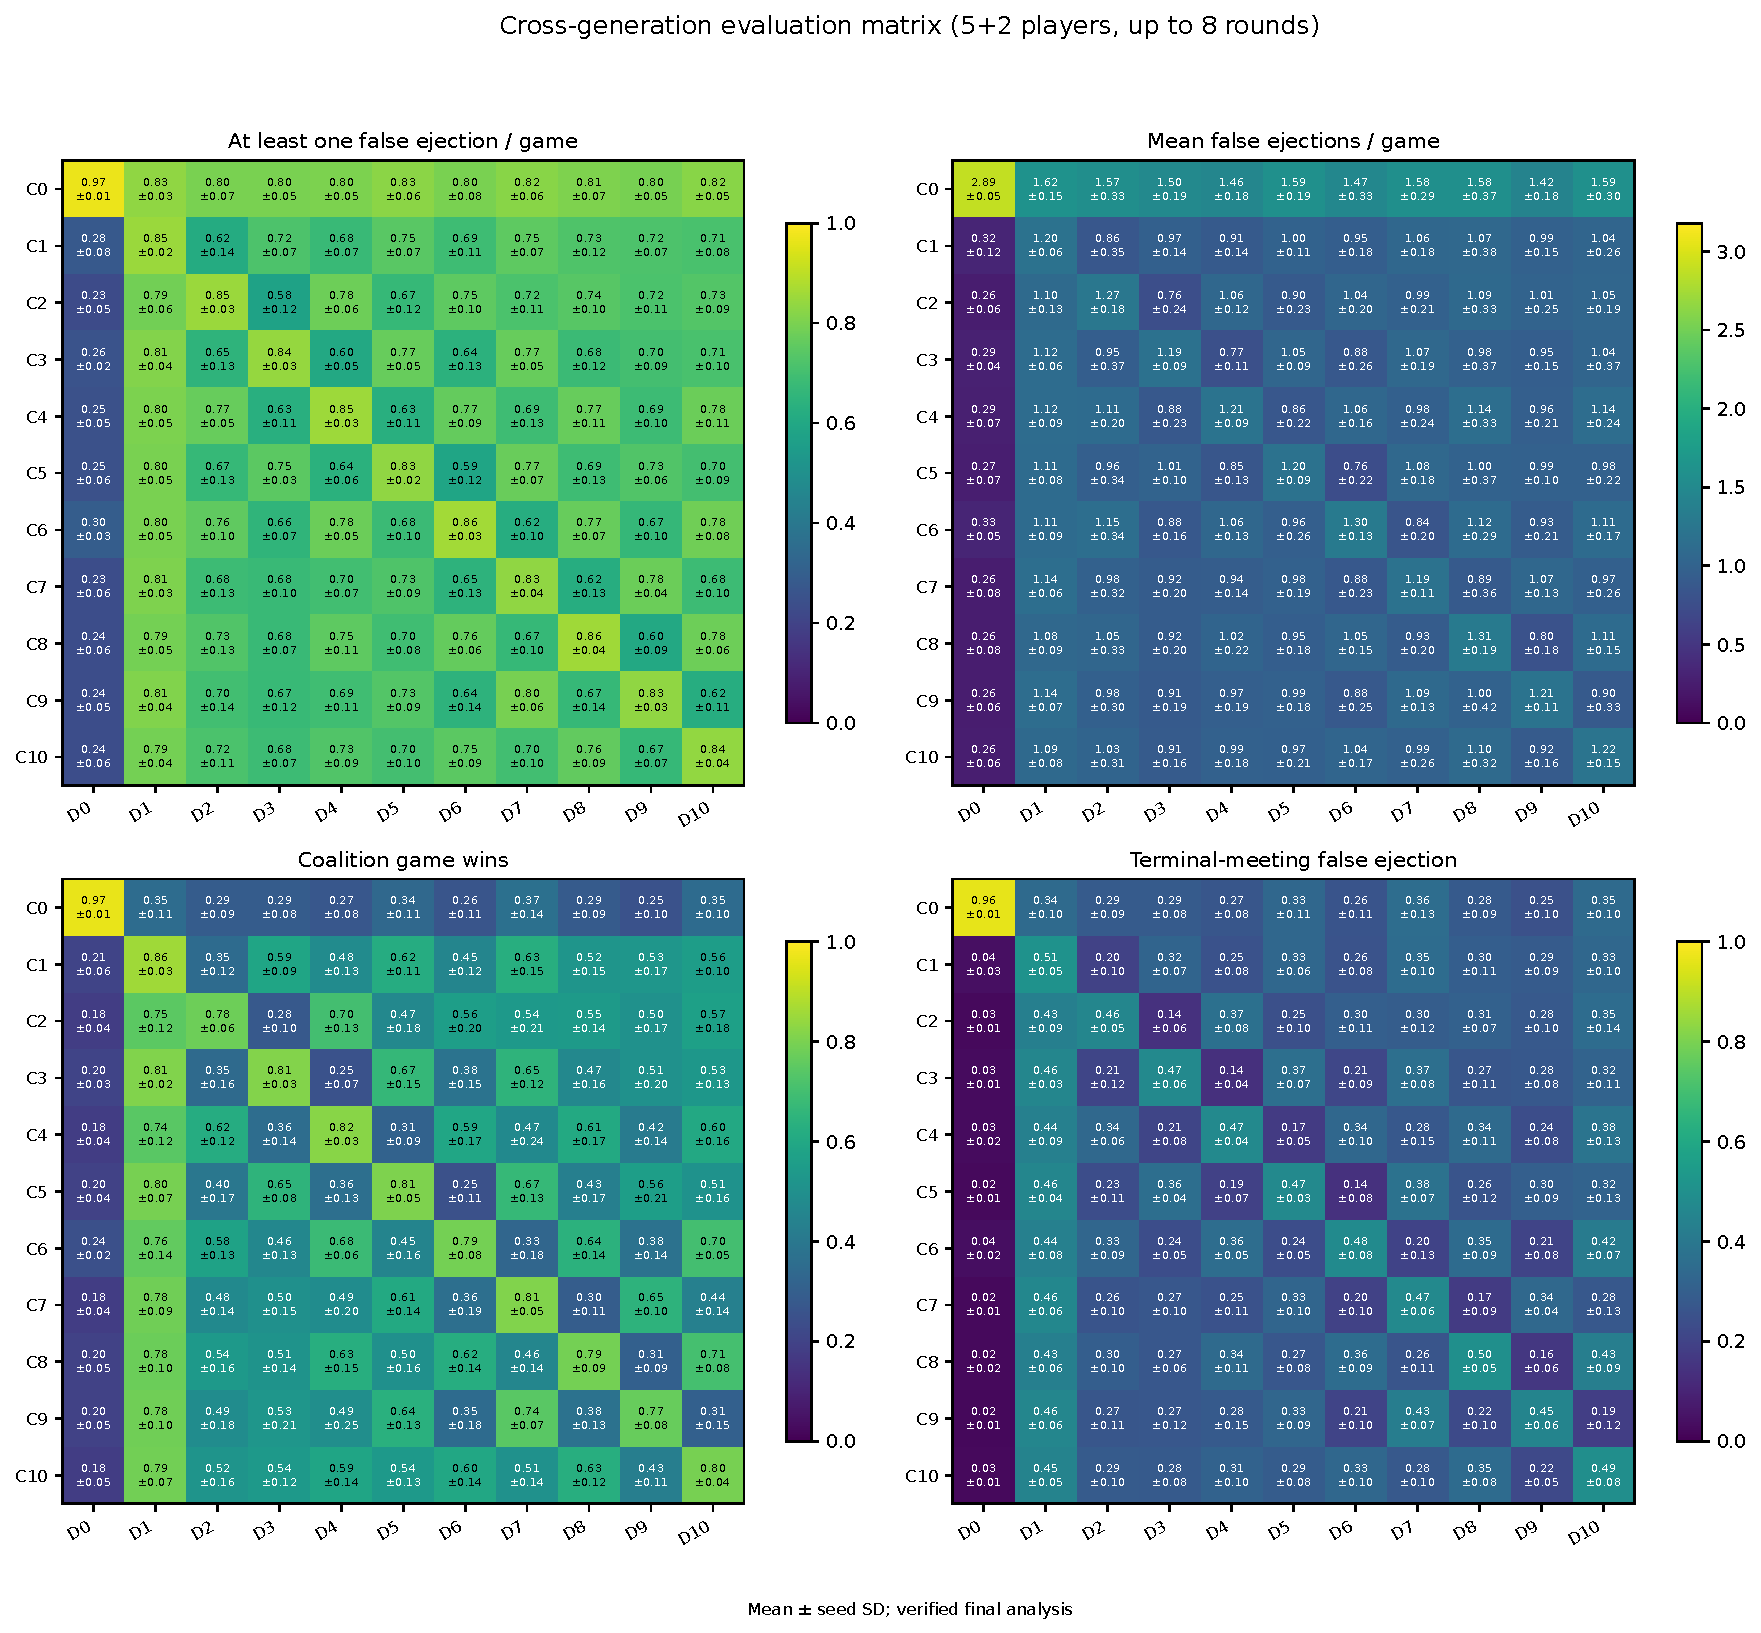
\includegraphics[width=1\linewidth,height=0.65\textheight]{figures/final/multigen_none_n7_r8_k10_matrix.pdf}
\caption{Figure 9. Full 5+2 multi-round crossplay, 500 episodes per cell
and ten seeds. Comparing each diagonal entry with the entry immediately
above measures adaptation against a fixed defender.}\label{fig:9}
\end{figure}

At 5+2, coalition victory is 0.9658 for C0--D0, 0.3524 for C0--D1, and
0.8562 for C1--D1. By generation ten it is 0.3068 for C9--D10 and 0.7968
for C10--D10, while C10--D0 achieves only 0.1804. The coalition
repeatedly improves against the newest defender, with limited transfer
to the scripted policy. The ten-seed loops' specified matrix-gain tests
pass Holm correction in the 25-test dynamics family (\(p=0.0488\)); the
five-seed largest-population loop does not. None of the specified
late-minus-early or parity tests rejects after correction.

\begin{figure}
\centering
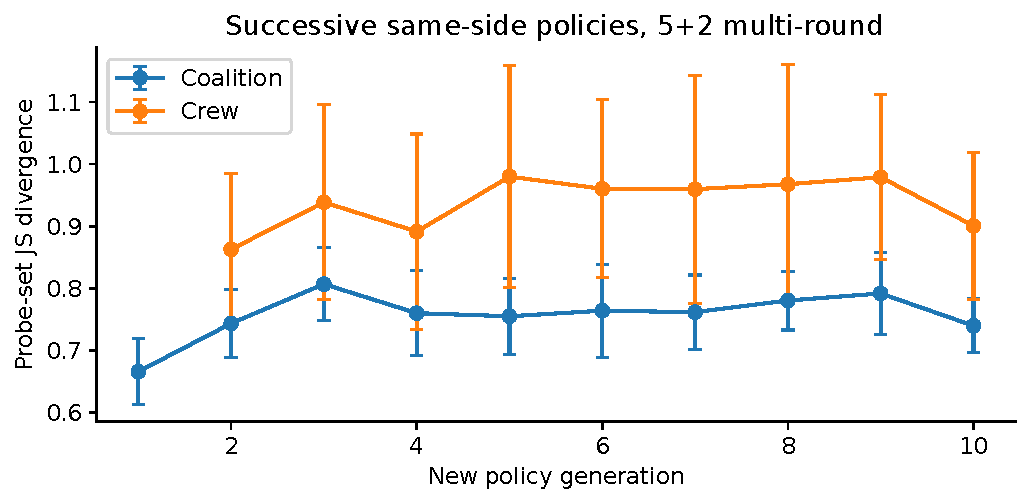
\includegraphics[width=1\linewidth,height=0.65\textheight]{figures/final/policy_distance.pdf}
\caption{Figure 10. Jensen--Shannon distances between successive
same-side policies on fixed probe observations, mean ± ten-seed SD.
Learned defender comparisons begin at D2 versus D1; D0 is scripted.
Distances reflect fresh initialization and training and are not
distances along a single continuous optimization
trajectory.}\label{fig:10}
\end{figure}

\begin{figure}
\centering
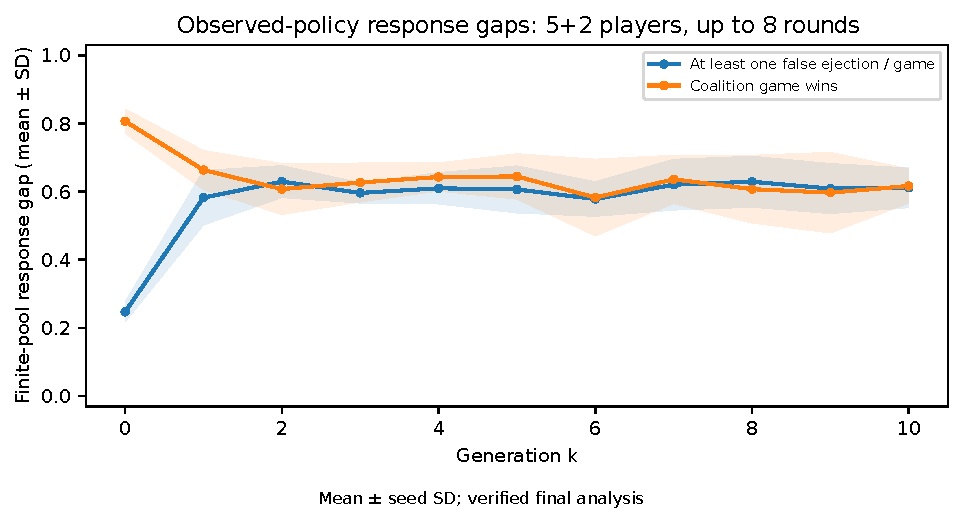
\includegraphics[width=1\linewidth,height=0.65\textheight]{figures/final/multigen_none_n7_r8_k10_response_gaps.pdf}
\caption{Figure 11. Retrospective response gaps in the finite observed
policy pool. Conservative simultaneous cell bands account for Monte
Carlo error and selection of extrema; later-generation policies are
included in earlier-generation pools.}\label{fig:11}
\end{figure}

Policy distances and outcome reversals do not identify an attracting
cycle. The policies are independently initialized at each stage, the
opponent changes, and outcome probabilities are estimated with finite
precision. A small observed gap can also reflect a limited policy pool.
These data describe repeated adaptive vulnerability within the measured
horizon, without proving convergence, nonconvergence, optimality, or
permanent attacker advantage.

\begin{figure}
\centering
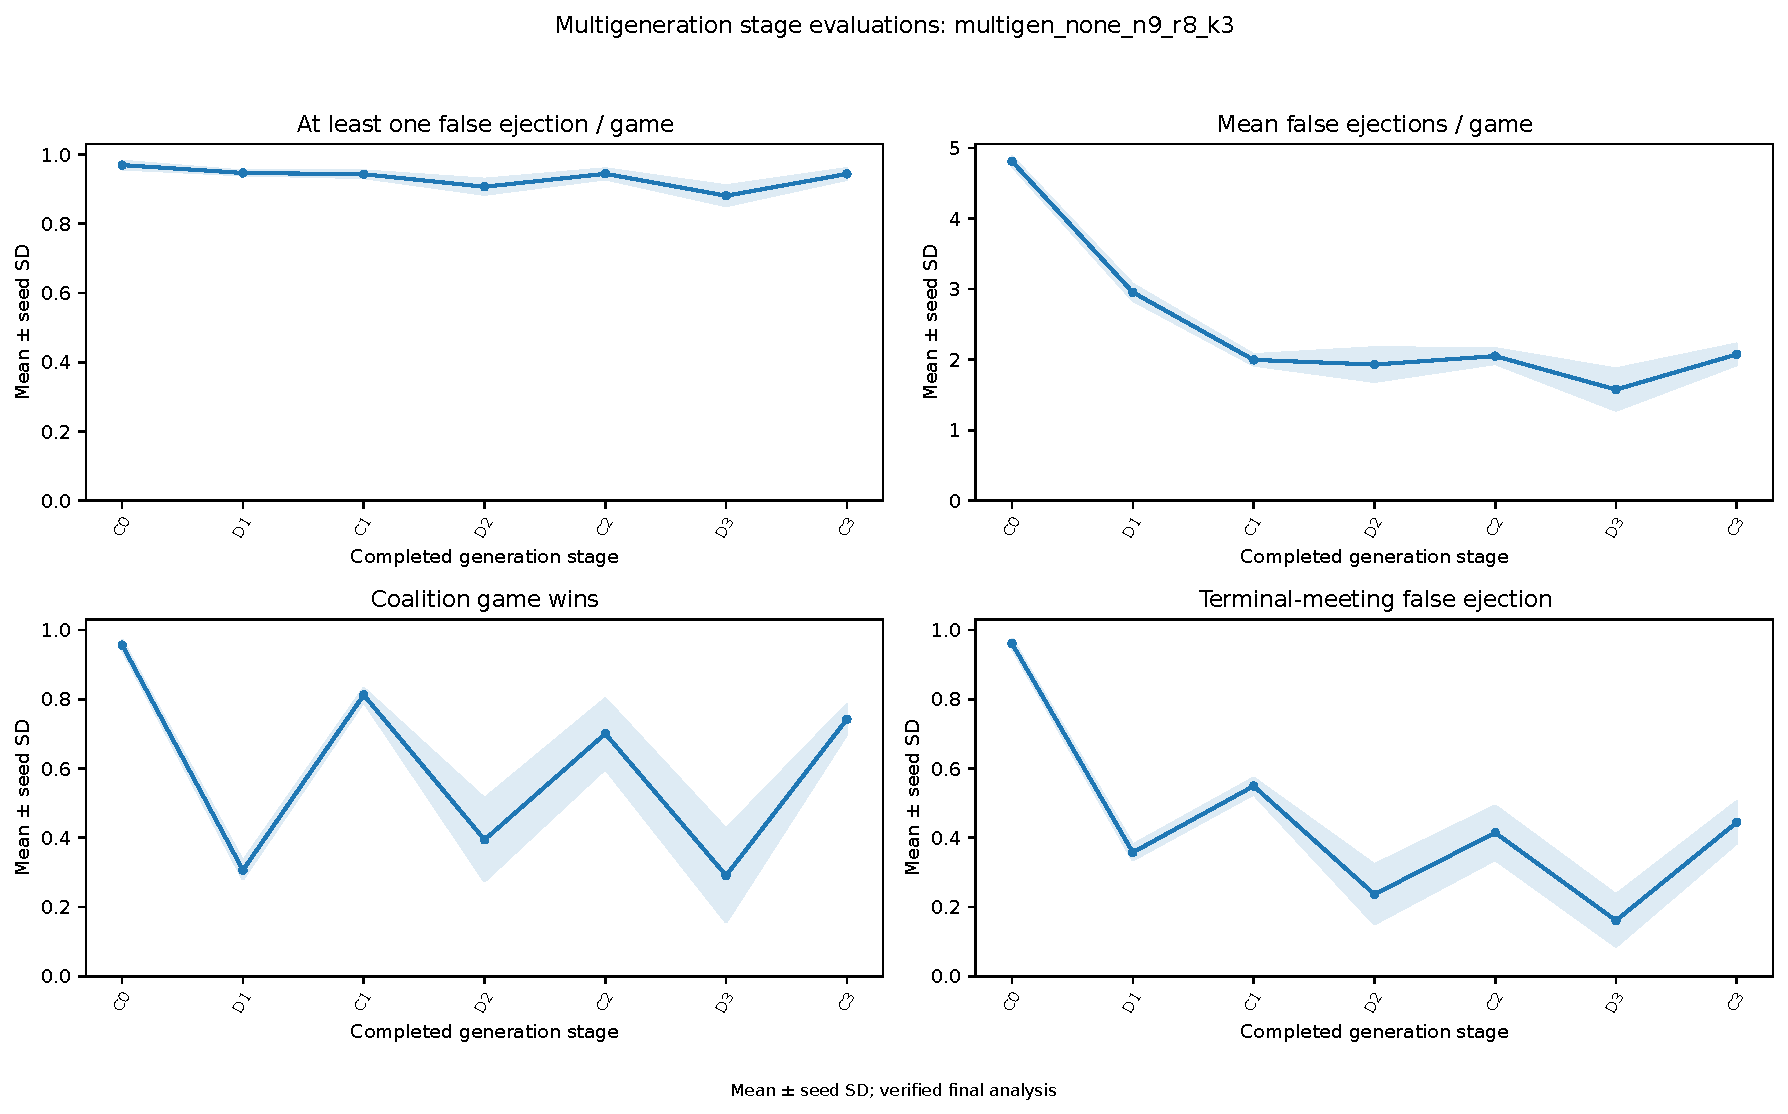
\includegraphics[width=1\linewidth,height=0.65\textheight]{figures/final/multigen_none_n9_r8_k3_stages.pdf}
\caption{Figure 12. Largest-population sequence, 7+2 players and three
generations across five seeds. This shorter horizon and coarser
statistical resolution limit comparison with ten-generation
results.}\label{fig:12}
\end{figure}

Two terminal coordination cells in the 7+2 loop are undefined because
all 500 games in each cell lost a coalition voter before the last
meeting. Complete meeting histories verify the zero denominator. No null
was replaced by zero, no seed was dropped, and all primary crossplay
outcomes remain complete. Terminal coordination should not be confused
with coordination over every meeting of a game.

\FloatBarrier

\subsection{F6: an analytical model of corroboration capture under
correlated
testimony}\label{f6-an-analytical-model-of-corroboration-capture-under-correlated-testimony}

The model isolates the one failure mode that the framing of
``credibility collapse'' usually refers to: manufactured agreement
earning a coalition more than its share of a trust rule's weight. We use
the term in that sense only; Section 6.2's corrected scripted
diagnostics do not show average coalition-weight amplification in those
conditions. The model replaces claims and votes by real-valued reports
about a latent state \(\theta\). \(n\) honest agents report
\(x_i = \theta + \varepsilon_i\) with
\(\varepsilon_i \sim \mathcal N(0,\sigma^2)\) i.i.d.; \(m\) coalition
agents report \(y_j = \theta + b + \eta_j\) with equicorrelated Gaussian
noise of marginal variance \(\sigma_c^2\), independent of honest noise,
and pairwise correlation \(\rho\) (\(\rho = 1\): identical, fully
coordinated reports); \(f = m/(n+m)\) is the coalition fraction. The
corroboration count \(c_i = \#\{k \neq i : |r_i - r_k| \le h\}\) is the
analogue of counting speakers whose claims are jointly satisfiable with
one's own, and the credibility-weighted estimate is
\(\hat\theta = \sum_i w_i r_i\) with \(w_i \propto e^{\gamma c_i}\),
gain \(\gamma = 1/\tau\). Because differences of Gaussians are Gaussian,
the pairwise agreement probabilities are explicit,
\(p_{HH} = \operatorname{erf}(h/2\sigma)\),
\(p_{CC}(\rho) = \operatorname{erf}\big(h/(2\sigma_c\sqrt{1-\rho})\big)\),
\(p_{CC}(1)=1\),
\(p_{HC}(b) = \Phi\big(\frac{h-b}{s}\big) - \Phi\big(\frac{-h-b}{s}\big)\)
with \(s^2 = \sigma^2 + \sigma_c^2\), and the expected corroboration
counts are \(\bar c_H = (n-1)p_{HH} + m\,p_{HC}\) and
\(\bar c_C = (m-1)p_{CC}(\rho) + n\,p_{HC}\). In mean field the
coalition's total weight is the logistic

\[
W_C(\gamma,\rho,f) = \frac{f}{f + (1-f)\,e^{-\gamma\,\Delta c(\rho)}},\qquad
\Delta c = \bar c_C - \bar c_H .
\]

Appendix A separates exact Gaussian agreement probabilities from a
deterministic mean-field surrogate obtained by applying softmax to
expected counts. For positive gain, the surrogate gives the coalition
more than its uniform share exactly when \(\Delta c>0\). For \(b\ne0\),
this increases its squared bias; its MSE also contains honest and
coalition variance. The Gaussian quantile
\(\sigma\Phi^{-1}(1/[2(1-f)])\) is an asymptotic reference for the
median's worst-case bias, so its intersection with \(W_C|b|\) is a bias
comparison, not a finite-sample error guarantee. With independent
repetitions, in the long-window limit and on a correlation interval with
\(p_{CC}\ge p_{HC}\) throughout, a dependence strength
\(\lambda\ge\gamma(m-1)(N-1)/n\) makes the defended surrogate's
coalition weight non-increasing with correlation on that interval, where
\(N=n+m\). The realized softmax can have a different amplification
boundary.

\begin{figure}
\centering
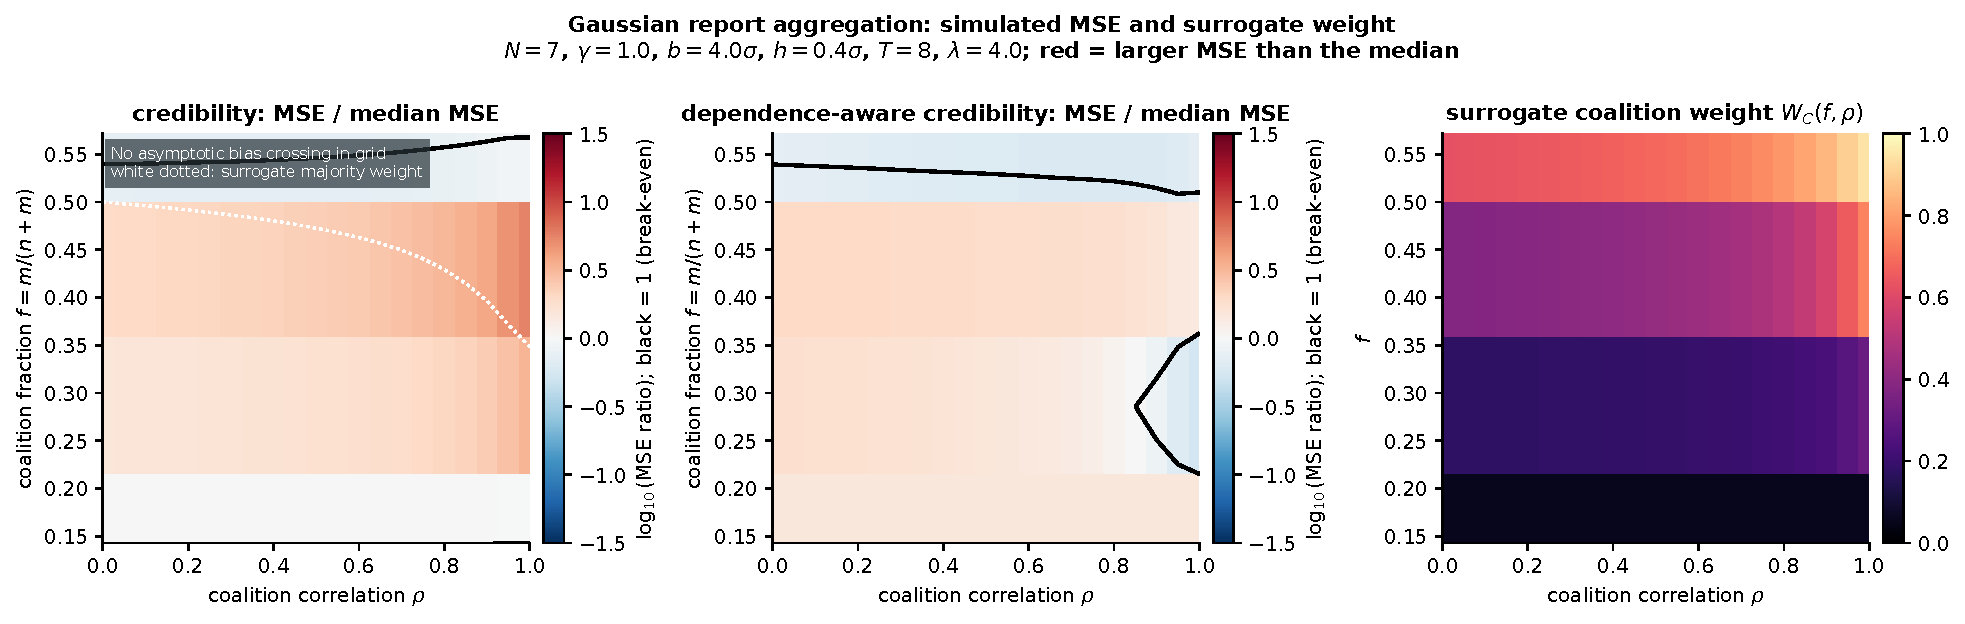
\includegraphics[width=1\linewidth,height=0.65\textheight]{figures/final/theory_phase.pdf}
\caption{Figure 13. Phase diagram of the model (\(N = 7\) reporters,
\(\gamma = 1\), \(b = 4\sigma\), \(h = 0.4\sigma\),
\(\sigma_c=\sigma\)). Rows are discrete coalition sizes,
\(f=1/7,2/7,3/7,4/7\); contours interpolate the sampled grid. The row
with \(f\ge1/2\) lies outside Appendix A's minority-coalition guarantee.
Colour: \(\log_{10}\) of the ratio of the estimator's error to the
median's; black contour: break-even; white reference contours, where
present, mark the surrogate's asymptotic bias-reference crossing and
majority-weight boundary. The N=7 grid has no bias-reference crossing.
These are analytical references, not exact boundaries for the realized
estimator. Left: credibility weighting; middle: dependence-aware
credibility (window of eight rounds, \(\lambda = 4\)); right: the
mean-field coalition weight \(W_C(f,\rho)\).}\label{fig:13}
\end{figure}

\begin{figure}
\centering
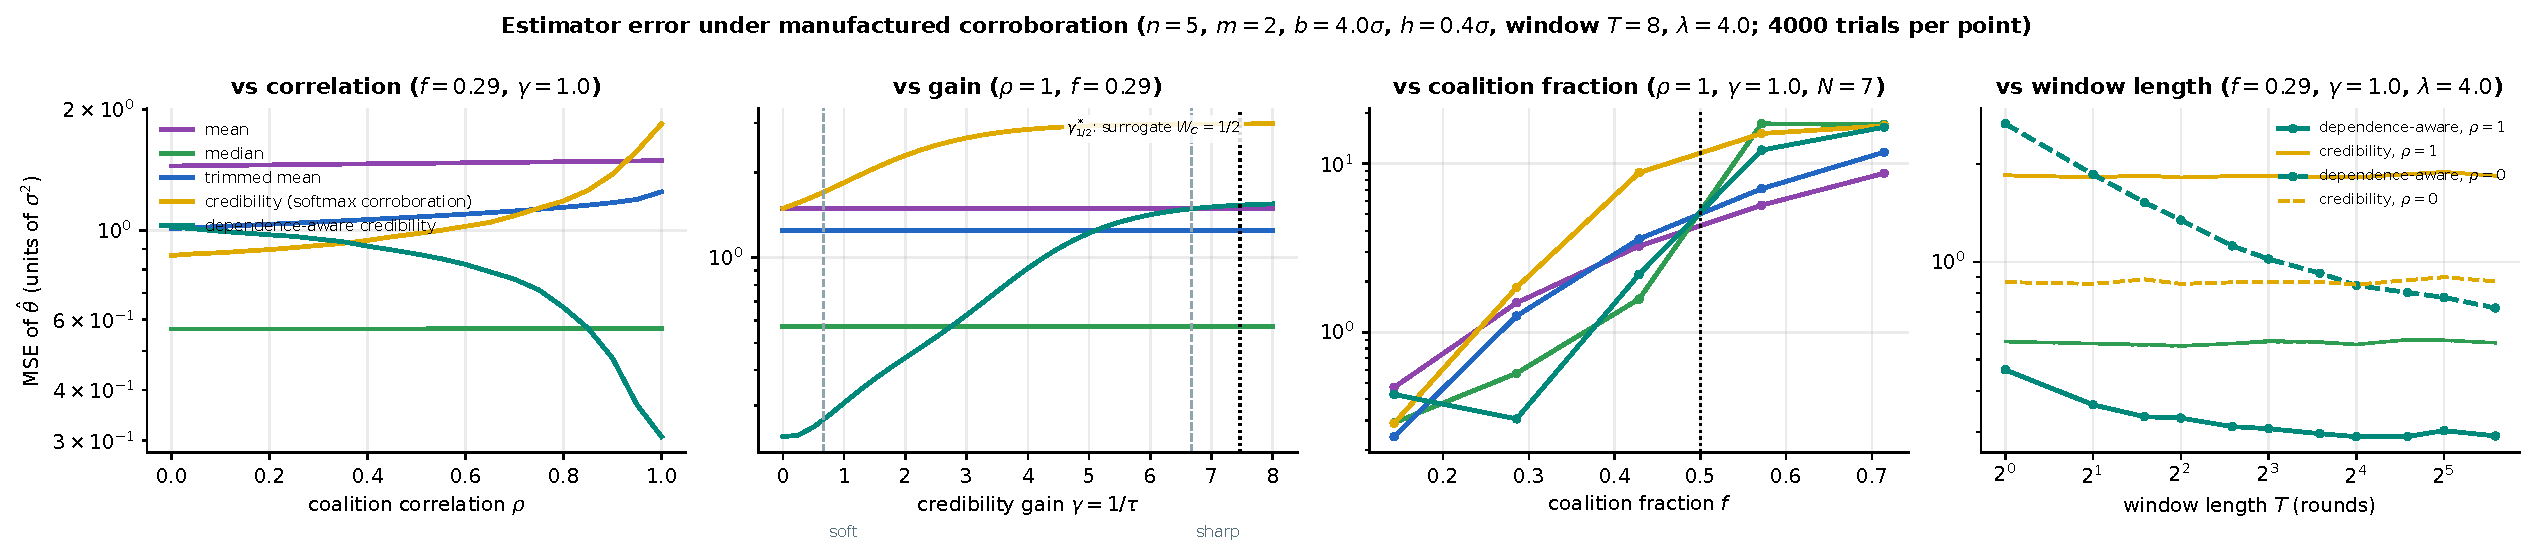
\includegraphics[width=1\linewidth,height=0.65\textheight]{figures/final/theory_error.pdf}
\caption{Figure 14. Estimator error (units of \(\sigma^2\)) against
coalition correlation, credibility gain (the game's soft and sharp gains
marked), coalition fraction, and the window length of the dependence
penalty; 5+2 defaults with \(\sigma_c=\sigma\), 4,000 trials per point.
The coalition-fraction sweep includes values outside the
minority-coalition guarantee.}\label{fig:14}
\end{figure}

Numerically, with \(n = 5\), \(m = 2\), \(\sigma_c=\sigma\),
\(h = 0.4\sigma\) (honest reporters agree with probability 0.22),
\(b = 4\sigma\) and \(\gamma = 1\), credibility weighting is the best
summing rule against \emph{independent} liars (mean-squared error 0.87
against 1.45 for the mean and 0.57 for the median) and the worst rule
against the \emph{same} liars coordinating (1.84 at \(\rho = 1\)), while
the median has similar rounded error at those endpoints (0.57): the
surrogate has \(\Delta c = -0.6\) at \(\rho = 0\) and \(+0.12\) at
\(\rho = 1\). The dependence-aware rule brings the coordinated case to
0.31, below the median, but pays for it at short windows and at low
correlation (1.02 at \(\rho = 0\)), because the concentration statistic
is estimated from few rounds. In the equal-variance, minority-coalition
surrogate, independent biased reporters cannot amplify their weight: at
\(\rho=0\), \(\Delta c=(n-m)(p_{HC}-p_{HH})\le0\). Unequal variances and
finite-sample softmax fluctuations require separate analysis. The median
retains a uniform bound in coalition bias whenever \(m<n\); this
worst-case guarantee is lost at one half, which does not mean every
estimator fails on every distribution.

Expected counts and expected weights can even predict different
directions of amplification. For \(n=5\), \(m=2\),
\(\sigma=\sigma_c=1\), \(b=20\), \(h=0.43\), \(\rho=1\), \(\gamma=1\),
the surrogate gives \(W_C=0.295>2/7\), while 100,000 Monte Carlo trials
give mean realized coalition weight 0.277, below the uniform share. The
model supplies a mechanism and analytical references; the game's
realized weights must be checked directly.

\textbf{Correspondence with the game.} The scripted mechanism diagnostic
directly measures lower average coalition weight than the uniform share
in the tested alibi cells. This is compatible with the surrogate's
prediction when honest agreement is high, but does not validate a
quantitative mapping from the Gaussian report model to symbolic
testimony. The game also subtracts caught-lying penalties from
credibility scores, so Table 5's scores are not pure pairwise agreement
counts. Neither the alibi-witness term nor the placement of the catch
penalty is represented in the Gaussian model. The measured game weights,
rather than the surrogate alone, establish the absence of average
coalition-weight amplification in those cells. The initial 3+2 game has
only 2+2 reporters after its incident victim is removed, so it lies
outside the proposition's strict-minority condition; the model's \(n\)
and \(m\) refer to actual reports, not initial players.

\textbf{A sensor-fusion analogue.} The rule was also applied to twelve
sensors reporting a drifting scalar, with three compromised sensors
(bias \(3\sigma\), \(\rho=1\), tolerance \(0.4\sigma\)). Across 20 runs,
credibility weighting assigns the coalition \(0.254\pm0.006\) of total
weight, only slightly above its uniform share of 0.25, compared with
\(0.099\pm0.004\) under independent compromised reports. Under
coordination its RMSE is \(0.99\pm0.03\,\sigma\), versus \(0.83\pm0.02\)
for the mean and \(0.58\pm0.02\) for the median. The dependence-aware
variant reduces coalition weight to \(0.044\) and RMSE to
\(0.56\pm0.01\,\sigma\). With independent compromised reports, the
median remains best (\(0.58\pm0.02\)), followed by credibility
(\(0.60\pm0.02\)), dependence-aware credibility (\(0.61\pm0.02\)), and
the mean (\(0.81\pm0.01\)). These simulations illustrate a benefit of
the dependence penalty under the chosen parameters; they do not
establish a general repair guarantee for trust aggregation.

\FloatBarrier

\subsection{F7: dependence-aware defense changes distinct outcomes
differently}\label{f7-dependence-aware-defense-changes-distinct-outcomes-differently}

\begin{figure}
\centering
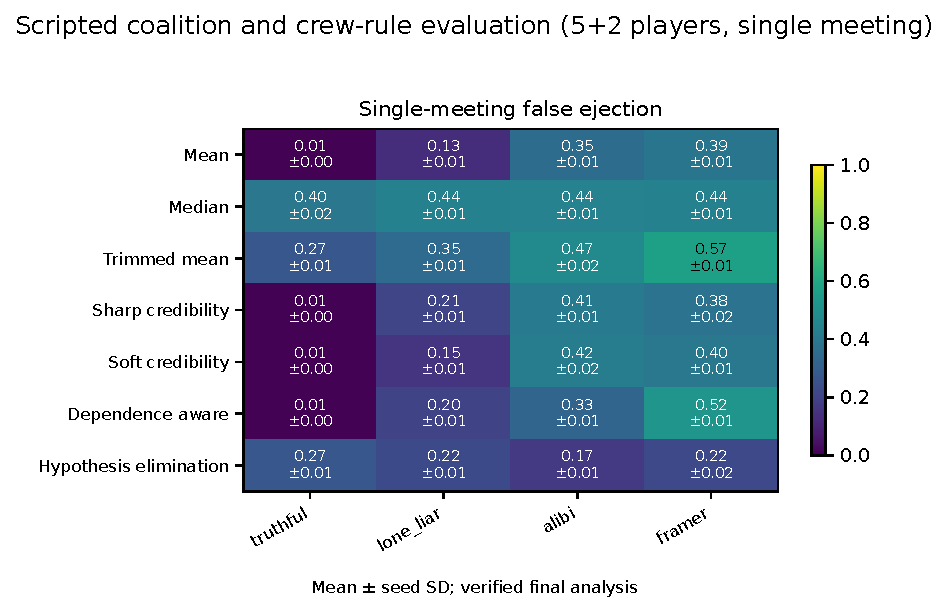
\includegraphics[width=1\linewidth,height=0.65\textheight]{figures/final/depstatic_n7_r1_rules.pdf}
\caption{Figure 15. Spatial static-rule evaluations at 5+2, five
evaluation replicates. This configuration has action-dependent evidence
and differs from F2's exogenous meeting-only evidence.}\label{fig:15}
\end{figure}

\FloatBarrier

\begin{table}[htbp]
\centering
\caption{Table 13. Spatial static false-ejection rates, mean ± SD across five
seeds. C0--C3 are frozen checkpoints from the single-meeting loop; no
rule is tuned by selecting its best test strength. The full seven-rule
and strength sweep is included with the data.}\label{tab:13}
\begin{tabular}{@{}
  >{\raggedright\arraybackslash}p{(\linewidth - 8\tabcolsep) * \real{0.2000}}
  >{\raggedleft\arraybackslash}p{(\linewidth - 8\tabcolsep) * \real{0.2000}}
  >{\raggedleft\arraybackslash}p{(\linewidth - 8\tabcolsep) * \real{0.2000}}
  >{\raggedleft\arraybackslash}p{(\linewidth - 8\tabcolsep) * \real{0.2000}}
  >{\raggedleft\arraybackslash}p{(\linewidth - 8\tabcolsep) * \real{0.2000}}@{}}
\toprule\noalign{}
\begin{minipage}[b]{\linewidth}\raggedright
Coalition
\end{minipage} & \begin{minipage}[b]{\linewidth}\raggedleft
Mean
\end{minipage} & \begin{minipage}[b]{\linewidth}\raggedleft
Soft
\end{minipage} & \begin{minipage}[b]{\linewidth}\raggedleft
Dependence
\end{minipage} & \begin{minipage}[b]{\linewidth}\raggedleft
Hypothesis
\end{minipage} \\
\midrule\noalign{}

Truthful & 0.007 ± 0.003 & 0.007 ± 0.003 & 0.007 ± 0.003 & 0.270 ±
0.010 \\
Lone & 0.132 ± 0.008 & 0.151 ± 0.011 & 0.204 ± 0.011 & 0.224 ± 0.014 \\
Alibi & 0.352 ± 0.013 & 0.421 ± 0.015 & 0.328 ± 0.012 & 0.168 ± 0.007 \\
Framer & 0.388 ± 0.011 & 0.399 ± 0.014 & 0.521 ± 0.014 & 0.222 ±
0.015 \\
C0 & 0.145 ± 0.068 & 0.193 ± 0.067 & 0.185 ± 0.072 & 0.111 ± 0.061 \\
C1 & 0.038 ± 0.014 & 0.074 ± 0.021 & 0.062 ± 0.020 & 0.057 ± 0.028 \\
C2 & 0.058 ± 0.018 & 0.092 ± 0.021 & 0.086 ± 0.022 & 0.061 ± 0.021 \\
C3 & 0.045 ± 0.016 & 0.080 ± 0.020 & 0.076 ± 0.023 & 0.050 ± 0.022 \\
\bottomrule\noalign{}
\end{tabular}
\end{table}

\FloatBarrier

\begin{table}[htbp]
\centering
\caption{Table 14. Adaptive dependence crossplay. Rule discounts testimony; rule
+ tally also discounts votes. Values are mean ± SD across ten seeds at
5+2 and five at 3+2, with 1,000 episodes per cell.}\label{tab:14}
\begin{tabular}{@{}lrrrr@{}}
\toprule\noalign{}
Players & Trained against & Soft & Rule & Rule + tally \\
\midrule\noalign{}

3+2 & soft & 0.210 ± 0.048 & 0.206 ± 0.038 & 0.413 ± 0.040 \\
3+2 & rule & 0.194 ± 0.030 & 0.226 ± 0.036 & 0.439 ± 0.016 \\
3+2 & both & 0.025 ± 0.006 & 0.039 ± 0.017 & 0.872 ± 0.010 \\
5+2 & soft & 0.194 ± 0.055 & 0.182 ± 0.051 & 0.204 ± 0.052 \\
5+2 & rule & 0.174 ± 0.031 & 0.170 ± 0.038 & 0.193 ± 0.034 \\
5+2 & both & 0.169 ± 0.038 & 0.164 ± 0.042 & 0.190 ± 0.040 \\
\bottomrule\noalign{}
\end{tabular}
\end{table}

\begin{figure}
\centering
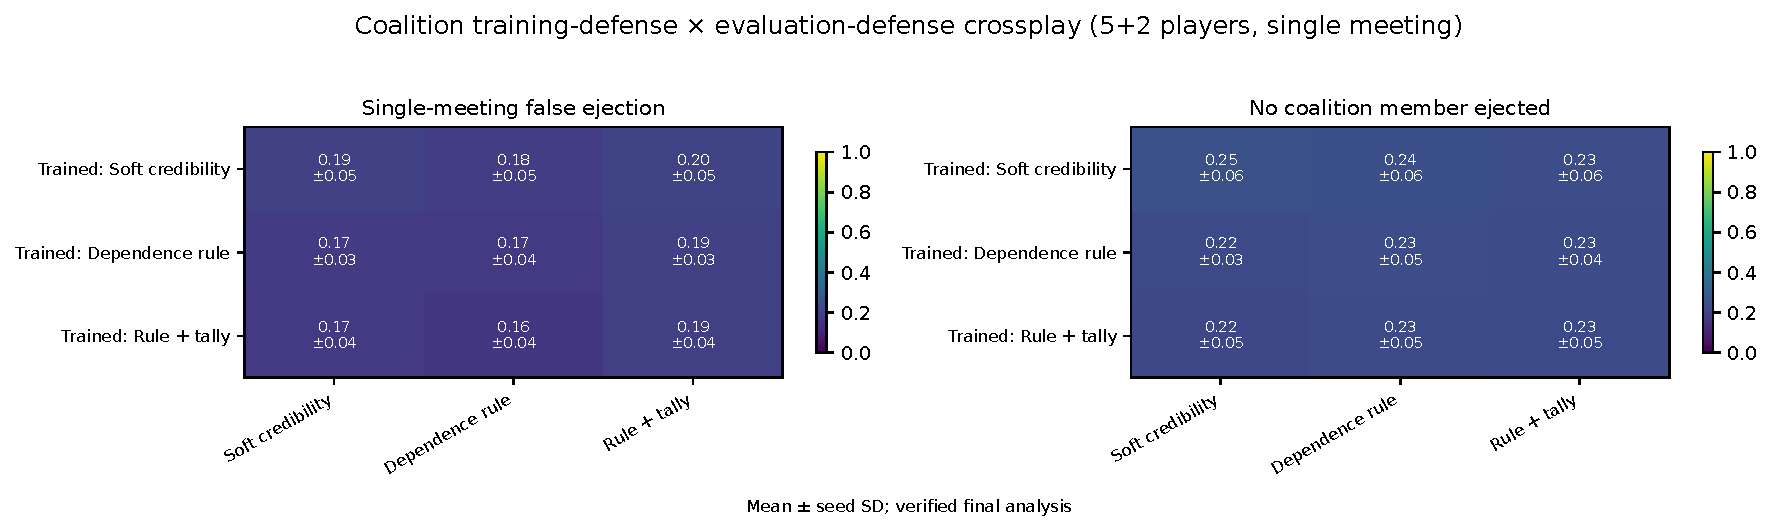
\includegraphics[width=1\linewidth,height=0.65\textheight]{figures/final/counterattack_n7_r1_crossplay.pdf}
\caption{Figure 16. Dependence-specific coalition training and transfer
at 5+2. Rows identify the training defense; columns identify the
evaluation defense.}\label{fig:16}
\end{figure}

At 5+2, rule-specific retraining gives false ejection 0.1696 against the
dependence rule, versus 0.1819 for the soft-trained coalition: effect
-0.0123, pointwise 95\% CI {[}-0.0516, 0.0374{]}, Holm-adjusted \(p=1\).
Against the combined rule/tally, retraining changes 0.2044 to 0.1896:
effect -0.0148, CI {[}-0.0513, 0.0215{]}, adjusted \(p=1\). These
corrected comparisons do not reproduce a general defense-specific attack
gain. At 3+2, however, the combined-defense rate rises descriptively
from 0.4132 to 0.8722; with five seeds the adjusted result remains
nonsignificant. Neither outcome establishes immunity.

\FloatBarrier

\begin{table}[htbp]
\centering
\caption{Table 15. Dependence-aware loop versus the undefended loop over the same
four generations and ten seeds. Difference is defended minus reference;
stages exclude C0. Means ± SD and adjusted tests retain the six-contrast
family.}\label{tab:15}
\begin{tabular}{@{}
  >{\raggedright\arraybackslash}p{(\linewidth - 10\tabcolsep) * \real{0.1667}}
  >{\raggedleft\arraybackslash}p{(\linewidth - 10\tabcolsep) * \real{0.1667}}
  >{\raggedleft\arraybackslash}p{(\linewidth - 10\tabcolsep) * \real{0.1667}}
  >{\raggedleft\arraybackslash}p{(\linewidth - 10\tabcolsep) * \real{0.1667}}
  >{\raggedleft\arraybackslash}p{(\linewidth - 10\tabcolsep) * \real{0.1667}}
  >{\raggedleft\arraybackslash}p{(\linewidth - 10\tabcolsep) * \real{0.1667}}@{}}
\toprule\noalign{}
\begin{minipage}[b]{\linewidth}\raggedright
Outcome
\end{minipage} & \begin{minipage}[b]{\linewidth}\raggedleft
Summary
\end{minipage} & \begin{minipage}[b]{\linewidth}\raggedleft
Reference
\end{minipage} & \begin{minipage}[b]{\linewidth}\raggedleft
Defended
\end{minipage} & \begin{minipage}[b]{\linewidth}\raggedleft
Difference
\end{minipage} & \begin{minipage}[b]{\linewidth}\raggedleft
Holm p
\end{minipage} \\
\midrule\noalign{}

Any FE & C stages & 0.847 ± 0.009 & 0.890 ± 0.007 & +0.042 & 0.0117 \\
Any FE & D stages & 0.658 ± 0.051 & 0.763 ± 0.047 & +0.104 & 0.0117 \\
Any FE & Matrix gain & 0.191 ± 0.051 & 0.129 ± 0.046 & -0.062 &
0.0234 \\
Coalition win & C stages & 0.817 ± 0.025 & 0.789 ± 0.026 & -0.029 &
0.0410 \\
Coalition win & D stages & 0.309 ± 0.065 & 0.348 ± 0.054 & +0.040 &
0.1387 \\
Coalition win & Matrix gain & 0.509 ± 0.086 & 0.445 ± 0.070 & -0.064 &
0.0469 \\
\bottomrule\noalign{}
\end{tabular}
\end{table}

\begin{figure}
\centering
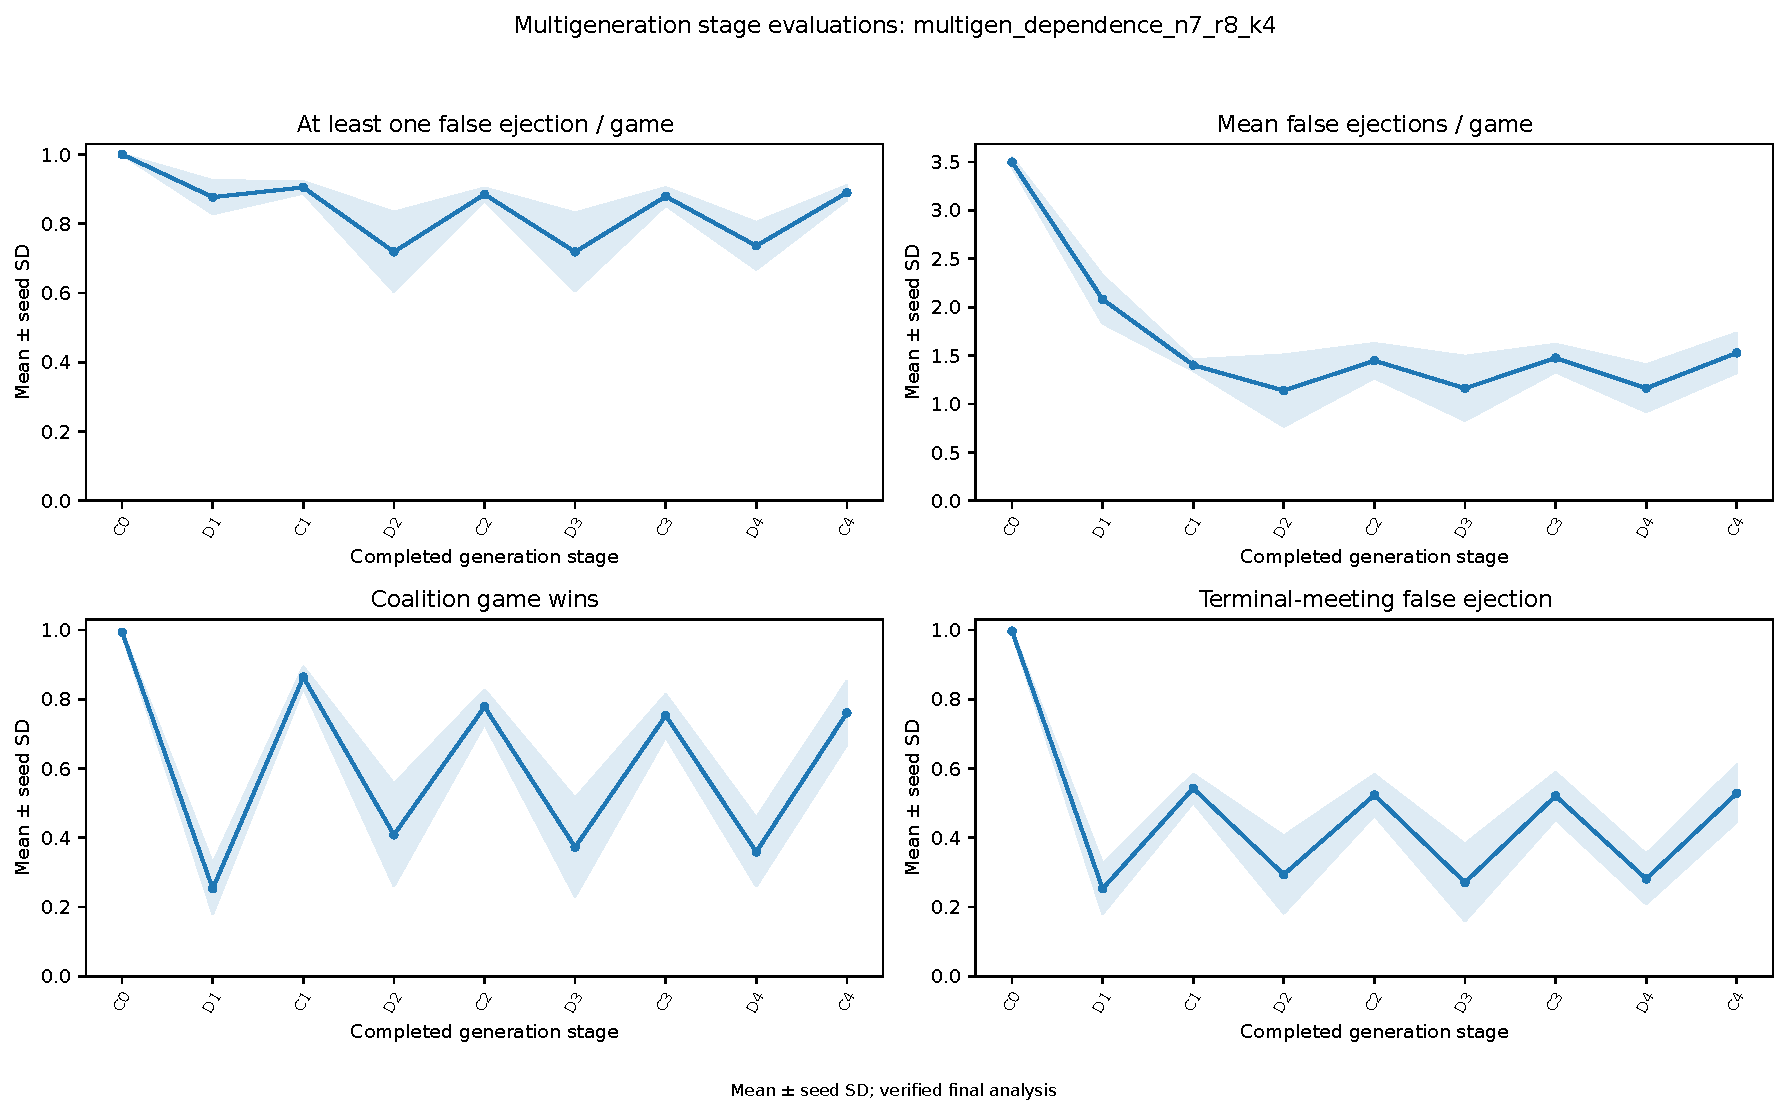
\includegraphics[width=1\linewidth,height=0.65\textheight]{figures/final/multigen_dependence_n7_r8_k4_stages.pdf}
\caption{Figure 17. The defended four-generation 5+2 multi-round
sequence. Table 15 compares it to the matching horizon and seeds of the
undefended sequence.}\label{fig:17}
\end{figure}

The dependence-aware loop increases any innocent ejection by 0.042425
after C stages (pointwise 95\% CI {[}0.034775, 0.049400{]}) and by
0.104375 after D stages ({[}0.073274, 0.135025{]}); both have
Holm-adjusted \(p=0.0117\). At C stages it reduces coalition victory by
0.028775 ({[}-0.045625, -0.012050{]}, adjusted \(p=0.0410\)). Matrix
adaptation gains also shrink, but this is not a guarantee of less harm
or better stability. The same defense can reduce one success measure
while increasing another adverse outcome.

\FloatBarrier

\subsection{F8: adaptive hypothesis attacks and ballot
diagnostics}\label{f8-adaptive-hypothesis-attacks-and-ballot-diagnostics}

\FloatBarrier

\begin{table}[htbp]
\centering
\caption{Table 16. Adaptive hypothesis crossplay, ten seeds at 5+2 and five at
7+2, 1,000 independent final episodes per cell. Training against a rule
is distinct from transferring a coalition trained against another rule.}\label{tab:16}
\begin{tabular}{@{}lrrrr@{}}
\toprule\noalign{}
Players & Trained against & Mean & Soft & Hypothesis \\
\midrule\noalign{}

5+2 & mean & 0.104 ± 0.037 & 0.148 ± 0.040 & 0.077 ± 0.031 \\
5+2 & soft & 0.143 ± 0.053 & 0.194 ± 0.055 & 0.126 ± 0.058 \\
5+2 & hypothesis & 0.096 ± 0.063 & 0.098 ± 0.068 & 0.422 ± 0.066 \\
7+2 & mean & 0.139 ± 0.051 & 0.189 ± 0.056 & 0.124 ± 0.074 \\
7+2 & soft & 0.136 ± 0.017 & 0.202 ± 0.013 & 0.110 ± 0.033 \\
7+2 & hypothesis & 0.037 ± 0.007 & 0.030 ± 0.007 & 0.604 ± 0.018 \\
\bottomrule\noalign{}
\end{tabular}
\end{table}

\begin{figure}
\centering
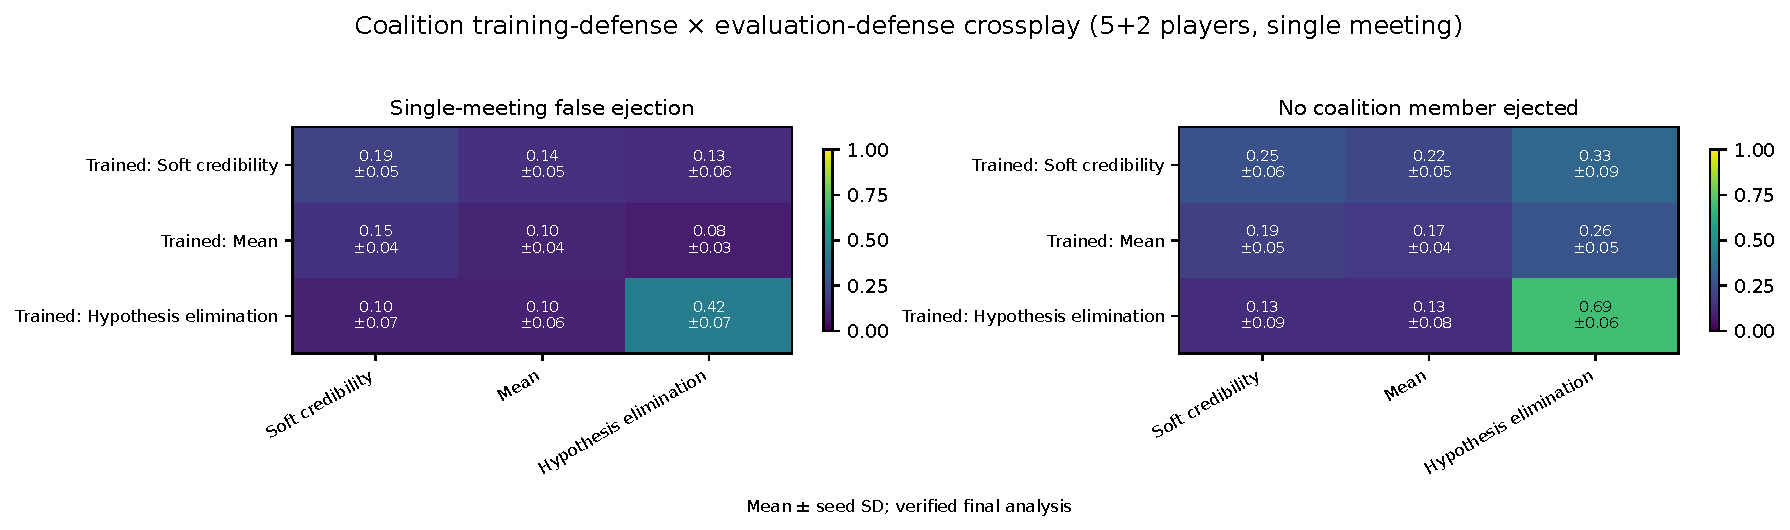
\includegraphics[width=1\linewidth,height=0.65\textheight]{figures/final/counterattack_hyp_n7_r1_crossplay.pdf}
\caption{Figure 18. Adaptive hypothesis attack and transfer at 5+2. The
matrix uses the main final-evaluation stream; the ballot supplement
below uses an independent stream.}\label{fig:18}
\end{figure}

At 5+2, targeted training increases hypothesis-defender false ejection
from 0.1255 to 0.4217: paired effect 0.2962, pointwise 95\% CI
{[}0.2521, 0.3418{]}, Holm-adjusted \(p=0.0273\). Its matched adaptive
error also exceeds soft-trained versus soft by 0.2275 (adjusted
\(p=0.0273\)). Yet the hypothesis-trained coalition achieves only 0.0962
against mean and 0.0976 against soft credibility. This is a substantial
tested adaptive vulnerability with opponent specialization, not a
uniformly stronger attack.

\FloatBarrier

\begin{landscape}

\begin{table}[p]
\centering
\caption{Table 17. Independent ballot supplement evaluated against the hypothesis
defender. Entries are means of within-seed rates; full SDs and
defined-seed counts accompany the data. Necessary: removing coalition
ballots prevents an observed false ejection. Sufficient: coalition
ballots alone select an innocent. Both condition on observed false
ejections and hold votes fixed; they are different counterfactuals. Top
score is the honest view's leading membership score, not a calibrated
probability.}\label{tab:17}
\begin{tabular}{@{}
  >{\raggedright\arraybackslash}p{(\linewidth - 16\tabcolsep) * \real{0.0800}}
  >{\raggedleft\arraybackslash}p{(\linewidth - 16\tabcolsep) * \real{0.1400}}
  >{\raggedleft\arraybackslash}p{(\linewidth - 16\tabcolsep) * \real{0.0750}}
  >{\raggedleft\arraybackslash}p{(\linewidth - 16\tabcolsep) * \real{0.1050}}
  >{\raggedleft\arraybackslash}p{(\linewidth - 16\tabcolsep) * \real{0.1050}}
  >{\raggedleft\arraybackslash}p{(\linewidth - 16\tabcolsep) * \real{0.1200}}
  >{\raggedleft\arraybackslash}p{(\linewidth - 16\tabcolsep) * \real{0.1200}}
  >{\raggedleft\arraybackslash}p{(\linewidth - 16\tabcolsep) * \real{0.1600}}
  >{\raggedleft\arraybackslash}p{(\linewidth - 16\tabcolsep) * \real{0.0950}}@{}}
\toprule\noalign{}
\begin{minipage}[b]{\linewidth}\raggedright
Players
\end{minipage} & \begin{minipage}[b]{\linewidth}\raggedleft
Attack
\end{minipage} & \begin{minipage}[b]{\linewidth}\raggedleft
FE
\end{minipage} & \begin{minipage}[b]{\linewidth}\raggedleft
Crew skip
\end{minipage} & \begin{minipage}[b]{\linewidth}\raggedleft
Top score
\end{minipage} & \begin{minipage}[b]{\linewidth}\raggedleft
Necessary
\end{minipage} & \begin{minipage}[b]{\linewidth}\raggedleft
Sufficient
\end{minipage} & \begin{minipage}[b]{\linewidth}\raggedleft
Crew-only FE
\end{minipage} & \begin{minipage}[b]{\linewidth}\raggedleft
Seeds
\end{minipage} \\
\midrule\noalign{}

5+2 & mean & 0.075 & 0.196 & 0.794 & 0.651 & 0.603 & 0.032 & 10 \\
5+2 & soft & 0.117 & 0.271 & 0.746 & 0.684 & 0.662 & 0.040 & 10 \\
5+2 & hypothesis & 0.424 & 0.661 & 0.507 & 0.973 & 0.978 & 0.014 & 10 \\
7+2 & mean & 0.128 & 0.448 & 0.683 & 0.770 & 0.769 & 0.027 & 5 \\
7+2 & soft & 0.101 & 0.406 & 0.713 & 0.819 & 0.823 & 0.022 & 5 \\
7+2 & hypothesis & 0.605 & 0.899 & 0.410 & 1.000 & 1.000 & 0.000 & 5 \\
\bottomrule\noalign{}
\end{tabular}
\end{table}

\end{landscape}

\begin{figure}
\centering
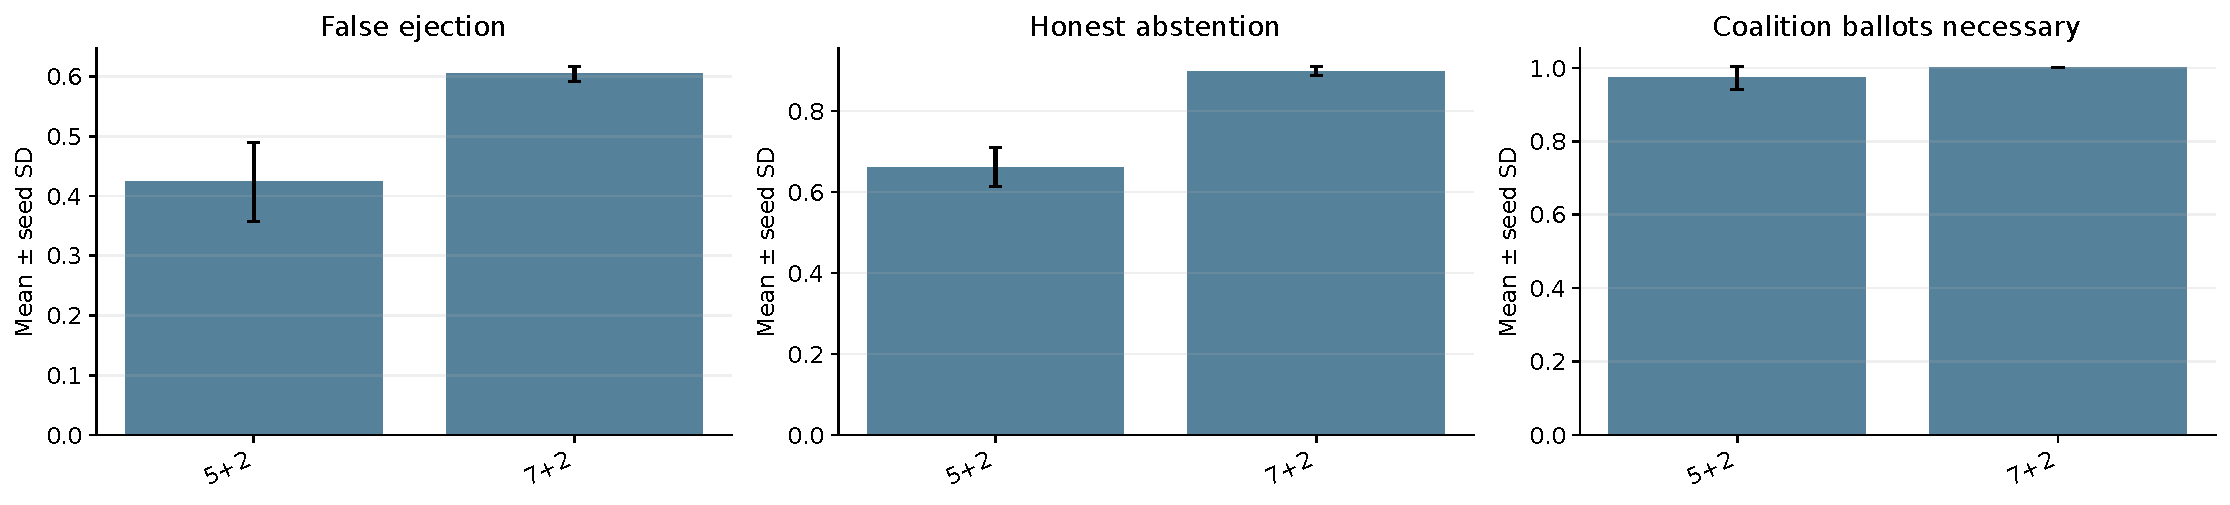
\includegraphics[width=1\linewidth,height=0.65\textheight]{figures/final/ballot_diagnostic.pdf}
\caption{Figure 19. Hypothesis-trained attacks against the hypothesis
rule in the independent ballot supplement. Means ± sample SD use ten
seeds at 5+2 and five at 7+2. Ballot necessity is conditional on a false
ejection.}\label{fig:19}
\end{figure}

The separate 135-cell, 67,500-episode diagnostic gives false ejection
0.4240 at 5+2 and 0.6048 at 7+2 for hypothesis-trained coalitions.
Honest voters skip at rates 0.6608 and 0.8988. Removing coalition
ballots prevents 97.26\% and 100\% of observed false ejections;
coalition ballots alone are sufficient in 97.75\% and 100\%. Crew-only
false ejection is 0.0142 and 0, respectively. Raw verification covers
the full electorate, including the ejected voter, and recomputes tally
and score-derived quantities.

These results support an abstention-related route to failure under
recorded votes. They do not show that abstention is the only cause, that
all score ties are uninformative, or that agents would retain their
votes if the decision rule changed. Membership scores are feasibility
summaries, not exact posterior probabilities; their numerical scale
alone does not establish calibrated uncertainty.

\FloatBarrier

\section{Interpretation}\label{interpretation}

The completed experiments distinguish three forms of evidence.
Scripted-rule comparisons measure behavior against specified testimony;
adaptive crossplay tests responses to particular trained opponents;
supplemental interventions investigate score and ballot mechanisms under
explicit matching assumptions. None replaces the others. The hypothesis
rule's scripted-attack benefits coexist with truthful-testimony costs
and targeted adaptive vulnerability.

Learning dynamics are also outcome-dependent. Multi-round defenders can
suppress coalition victory while retaining frequent innocent ejections.
The dependence-aware loop modestly lowers coalition victory after
coalition stages yet increases whole-game voting harm. A smaller
adaptation gap is therefore not itself a safety improvement or a
stability certificate. The ten-generation sequence shows repeated gains
against the latest opponent; fresh initialization, restricted policy
classes, changing opponents, and finite evaluation prevent an asymptotic
dynamical conclusion.

The Gaussian surrogate models corroboration capture as coalition-weight
amplification. The game's measured alibi errors occur while total
coalition weight remains below its uniform share in the inspected
scripted records. Alibi credit and the placement of self-incriminating
penalties within downweighted rows offer different mechanisms, with
attack-dependent tradeoffs under intervention. This distinction prevents
the paper's motivating analogy from becoming an unsupported explanation
of every game outcome.

\FloatBarrier

\section{Limitations}\label{limitations}

\begin{enumerate}
\def\labelenumi{\arabic{enumi}.}
\tightlist
\item
  \textbf{Restricted benchmark.} Small maps, structured claims, two
  policy-sharing impostors, and fixed observation/action spaces do not
  establish behavior in natural-language deliberation, independently
  incentivized coalitions, or deployed sensor systems.
\item
  \textbf{Finite learning and testing.} PPO stages start from fresh
  weights and have finite budgets. Crossplay contains a finite policy
  pool, not optimal responses over all possible strategies. The larger
  population has only three generations and five seeds.
\item
  \textbf{Inference resolution.} Five-seed exact tests cannot reject at
  raw 0.05, and larger ten-seed families encounter a corresponding Holm
  limit. Intervals are pointwise; Holm correction is within named
  families. Absence of rejection is not equivalence, and 303 specified
  contrasts do not make the original exploratory study prospectively
  preregistered.
\item
  \textbf{Information and hypothesis modeling.} Within-round histories
  are matched, but non-recurrent actors have limited cross-round memory.
  Hidden-partner controls change several information channels together.
  The hypothesis solver is exact for emitted constraints, with
  documented relaxations for some negative claims; normalized
  feasibility scores are not calibrated generative posteriors.
\item
  \textbf{Mechanism scope.} Matched initial evidence does not fix
  subsequent responses; ballot removal does not model behavioral
  adaptation. The bounded F2 replay does not estimate failure-route
  prevalence. Supplemental studies remain descriptive.
\item
  \textbf{Outcome definitions.} Creator quantities require incidents.
  Terminal coordination can be undefined after a prior coalition
  ejection. Whole-game harm includes incident-free meetings. Voting
  error, abstention, and coalition victory cannot be substituted for one
  another.
\item
  \textbf{Implementation and reproduction.} The audit changed several
  components together, so differences from historical experiments cannot
  be attributed to one isolated fix. Frozen source hashes, checkpoints,
  raw outcomes, and environment manifests support reproduction;
  different operating systems and PyTorch builds need not produce
  bit-identical training.
\item
  \textbf{Analytical correspondence.} The Gaussian surrogate has a
  strict reporter-minority condition and a parameter-restricted
  dependence result. Finite-sample weights and game testimony need not
  obey its amplification thresholds.
\end{enumerate}

\FloatBarrier

\section{Conclusion}\label{conclusion}

The completed corrected replication shows that defensive performance
depends on the attacker, the training sequence, and the chosen outcome.
Coalition learning increases harmful aligned voting without increasing
directly false claims. Hypothesis scoring trades some scripted-attack
accuracy gains for truthful-testimony costs and remains vulnerable to
targeted training. Repeated response learning produces renewed gains
against the latest opponent over the observed horizon, without
establishing an equilibrium or persistent cycle. Dependence-aware
defenses can lower coalition victory while increasing innocent
ejections. Combining explicit outcome definitions, adaptive crossplay,
and bounded mechanism diagnostics yields a more qualified account of
coalition deception than any single credibility or win-rate measure.

\FloatBarrier

\section*{Acknowledgements}\label{acknowledgements}
\addcontentsline{toc}{section}{Acknowledgements}

OpenAI Codex, using GPT-6, assisted with implementation review,
correction and testing of research code, numerical reanalysis, and
manuscript editing. Numerical measurements were produced by the
executable experiments and analysis scripts described in this paper.

\FloatBarrier

\section*{Data availability}\label{data-availability}
\addcontentsline{toc}{section}{Data availability}

Code, the manuscript, all final seed-level summaries, planned
comparisons, and supplemental diagnostics are available in the public
repository
\href{https://github.com/IsaacLin247/coalition-deception}{Coalition
Deception}. The versioned corrected-study release supplies the original
frozen source, retained checkpoints, raw episode and meeting records,
and checksum manifests:
\href{https://github.com/IsaacLin247/coalition-deception/releases/tag/corrected-study-2026-09-11}{corrected-study-2026-09-11}.
The original and portable source fingerprints are distinguished in the
reproduction guide. Appendix C specifies the analysis and manuscript
build.

\FloatBarrier

\section*{References}\label{references}
\addcontentsline{toc}{section}{References}

\protect\phantomsection\label{refs}
\begin{CSLReferences}{0}{0}
\bibitem[\citeproctext]{ref-crawford1982}
\CSLLeftMargin{{[}1{]} }%
\CSLRightInline{V. P. Crawford and J. Sobel, {``Strategic information
transmission,''} \emph{Econometrica}, vol. 50, no. 6, pp. 1431--1451,
1982, doi: \href{https://doi.org/10.2307/1913390}{10.2307/1913390}.}

\bibitem[\citeproctext]{ref-lewis1969}
\CSLLeftMargin{{[}2{]} }%
\CSLRightInline{D. Lewis, \emph{Convention: A philosophical study}.
Harvard University Press, 1969.}

\bibitem[\citeproctext]{ref-kharitonov2019}
\CSLLeftMargin{{[}3{]} }%
\CSLRightInline{E. Kharitonov, R. Chaabouni, D. Bouchacourt, and M.
Baroni, {``{EGG}: A toolkit for research on emergence of lanGuage in
games,''} in \emph{Proceedings of the 2019 conference on empirical
methods in natural language processing and the 9th international joint
conference on natural language processing: System demonstrations}, 2019,
pp. 55--60. doi:
\href{https://doi.org/10.18653/v1/D19-3010}{10.18653/v1/D19-3010}.}

\bibitem[\citeproctext]{ref-condorelli2024}
\CSLLeftMargin{{[}4{]} }%
\CSLRightInline{D. Condorelli and M. Furlan, {``Cheap talking
algorithms.''} 2024. Available:
\url{https://arxiv.org/abs/2310.07867v6}}

\bibitem[\citeproctext]{ref-chen2025}
\CSLLeftMargin{{[}5{]} }%
\CSLRightInline{K. Chen, {``Communication with multiple senders.''}
2025. Available: \url{https://arxiv.org/abs/2505.14639v1}}

\bibitem[\citeproctext]{ref-arieli2023}
\CSLLeftMargin{{[}6{]} }%
\CSLRightInline{I. Arieli, I. Geffner, and M. Tennenholtz, {``Resilient
information aggregation,''} in \emph{Proceedings of the 19th conference
on theoretical aspects of rationality and knowledge (TARK)}, in
Electronic proceedings in theoretical computer science, vol. 379. 2023,
pp. 31--45. doi:
\href{https://doi.org/10.4204/EPTCS.379.6}{10.4204/EPTCS.379.6}.}

\bibitem[\citeproctext]{ref-figura2021}
\CSLLeftMargin{{[}7{]} }%
\CSLRightInline{M. Figura, Y. Lin, J. Liu, and V. Gupta, {``Resilient
consensus-based multi-agent reinforcement learning with function
approximation.''} 2021. Available:
\url{https://arxiv.org/abs/2111.06776}}

\bibitem[\citeproctext]{ref-witkowski2012}
\CSLLeftMargin{{[}8{]} }%
\CSLRightInline{J. Witkowski and D. C. Parkes, {``A robust {B}ayesian
truth serum for small populations,''} in \emph{Proceedings of the 26th
AAAI conference on artificial intelligence}, 2012, pp. 1492--1498. doi:
\href{https://doi.org/10.1609/aaai.v26i1.8261}{10.1609/aaai.v26i1.8261}.}

\bibitem[\citeproctext]{ref-elmhamdi2023}
\CSLLeftMargin{{[}9{]} }%
\CSLRightInline{E.-M. El-Mhamdi, S. Farhadkhani, R. Guerraoui, and L.-N.
Hoang, {``On the strategyproofness of the geometric median,''} in
\emph{Proceedings of the 26th international conference on artificial
intelligence and statistics (AISTATS)}, in Proceedings of machine
learning research, vol. 206. 2023, pp. 2603--2640. Available:
\url{https://proceedings.mlr.press/v206/el-mhamdi23a.html}}

\bibitem[\citeproctext]{ref-kopparapu2022}
\CSLLeftMargin{{[}10{]} }%
\CSLRightInline{K. Kopparapu \emph{et al.}, {``Hidden agenda: A social
deduction game with diverse learned equilibria.''} 2022. Available:
\url{https://arxiv.org/abs/2201.01816}}

\bibitem[\citeproctext]{ref-sarkar2025}
\CSLLeftMargin{{[}11{]} }%
\CSLRightInline{B. Sarkar, W. Xia, C. K. Liu, and D. Sadigh, {``Training
language models for social deduction with multi-agent reinforcement
learning,''} in \emph{Proceedings of the 24th international conference
on autonomous agents and multiagent systems (AAMAS)}, 2025, pp.
1830--1839. doi:
\href{https://doi.org/10.65109/PHJJ9903}{10.65109/PHJJ9903}.}

\bibitem[\citeproctext]{ref-blumenkamp2021}
\CSLLeftMargin{{[}12{]} }%
\CSLRightInline{J. Blumenkamp and A. Prorok, {``The emergence of
adversarial communication in multi-agent reinforcement learning,''} in
\emph{Proceedings of the 2020 conference on robot learning}, in
Proceedings of machine learning research, vol. 155. 2021, pp.
1394--1414. Available:
\url{https://proceedings.mlr.press/v155/blumenkamp21a.html}}

\bibitem[\citeproctext]{ref-li2021}
\CSLLeftMargin{{[}13{]} }%
\CSLRightInline{J. Li \emph{et al.}, {``Shapley counterfactual credits
for multi-agent reinforcement learning,''} in \emph{Proceedings of the
27th ACM SIGKDD conference on knowledge discovery and data mining},
2021, pp. 934--942. doi:
\href{https://doi.org/10.1145/3447548.3467420}{10.1145/3447548.3467420}.}

\bibitem[\citeproctext]{ref-orzan2024}
\CSLLeftMargin{{[}14{]} }%
\CSLRightInline{N. Orzan, E. Acar, D. Grossi, and R. Rădulescu,
{``Emergent cooperation under uncertain incentive alignment,''} in
\emph{Proceedings of the 23rd international conference on autonomous
agents and multiagent systems (AAMAS)}, 2024, pp. 1521--1530. Available:
\url{https://arxiv.org/abs/2401.12646}}

\bibitem[\citeproctext]{ref-motwani2024}
\CSLLeftMargin{{[}15{]} }%
\CSLRightInline{S. R. Motwani \emph{et al.}, {``Secret collusion among
{AI} agents: Multi-agent deception via steganography,''} in
\emph{Advances in neural information processing systems 37 (NeurIPS)},
2024. doi:
\href{https://doi.org/10.52202/079017-2336}{10.52202/079017-2336}.}

\bibitem[\citeproctext]{ref-tramer2020}
\CSLLeftMargin{{[}16{]} }%
\CSLRightInline{F. Tramèr, N. Carlini, W. Brendel, and A. Madry, {``On
adaptive attacks to adversarial example defenses,''} in \emph{Advances
in neural information processing systems}, 2020. Available:
\url{https://arxiv.org/abs/2002.08347}}

\bibitem[\citeproctext]{ref-lanctot2017}
\CSLLeftMargin{{[}17{]} }%
\CSLRightInline{M. Lanctot \emph{et al.}, {``A unified game-theoretic
approach to multiagent reinforcement learning,''} in \emph{Advances in
neural information processing systems}, 2017. Available:
\url{https://arxiv.org/abs/1711.00832}}

\bibitem[\citeproctext]{ref-schulman2017}
\CSLLeftMargin{{[}18{]} }%
\CSLRightInline{J. Schulman, F. Wolski, P. Dhariwal, A. Radford, and O.
Klimov, {``Proximal policy optimization algorithms.''} 2017. Available:
\url{https://arxiv.org/abs/1707.06347}}

\bibitem[\citeproctext]{ref-huang2022}
\CSLLeftMargin{{[}19{]} }%
\CSLRightInline{S. Huang and S. Ontañón, {``A closer look at invalid
action masking in policy gradient algorithms,''} in \emph{Proceedings of
the international FLAIRS conference}, 2022. doi:
\href{https://doi.org/10.32473/flairs.v35i.130584}{10.32473/flairs.v35i.130584}.}

\end{CSLReferences}

\FloatBarrier

\section*{Appendix A. Proposition: corroboration capture under
correlated
testimony}\label{appendix-a.-proposition-corroboration-capture-under-correlated-testimony}
\addcontentsline{toc}{section}{Appendix A. Proposition: corroboration
capture under correlated testimony}

\textbf{Setting.} Let \(1\le m<n\), \(N=n+m\), \(f=m/N\),
\(\sigma,\sigma_c,h>0\), \(\gamma,\lambda\ge0\), and \(\rho\in[0,1]\).
Honest reports are \(x_i=\theta+\varepsilon_i\) with independent
\(\varepsilon_i\sim\mathcal N(0,\sigma^2)\). Coalition reports are
\(y_j=\theta+b+\eta_j\), with
\(\eta\sim\mathcal N(0,\sigma_c^2[(1-\rho)I+\rho\mathbf1\mathbf1^\top])\),
independent of the honest noise. Define \(r=(x,y)\),
\(c_i=\#\{k\ne i:|r_i-r_k|\le h\}\), and the realized estimator
\(\hat\theta_{\rm cred}=\sum_i w_i r_i\), \(w_i\propto e^{\gamma c_i}\).
Dependence-aware weights additionally multiply by
\(e^{-\lambda\mathrm{ex}_i}\), where
\(\mathrm{ex}_i=\max_{k\ne i}D_{ik}-(N-1)^{-1}\sum_{k\ne i}D_{ik}\) and
\(D_{ik}\) is the agreement frequency across \(T\) independent
repetitions with fixed model parameters.

\textbf{Exact agreement probabilities.} With
\(s^2=\sigma^2+\sigma_c^2\), \[
p_{HH}=\operatorname{erf}(h/(2\sigma)),\qquad
p_{CC}(\rho)=\operatorname{erf}\!\left(\frac{h}{2\sigma_c\sqrt{1-\rho}}\right),\quad p_{CC}(1)=1,
\] \[
p_{HC}=\Phi((h-b)/s)-\Phi((-h-b)/s).
\] Hence \(\bar c_H=(n-1)p_{HH}+mp_{HC}\),
\(\bar c_C=(m-1)p_{CC}+np_{HC}\) and \(\Delta c=\bar c_C-\bar c_H\) is
non-decreasing in \(\rho\).

\textbf{Deterministic mean-field surrogate.} Replace each random
corroboration count by its group expectation. The resulting coalition
weight and estimator are \[
W_C=\frac{f}{f+(1-f)e^{-\gamma\Delta c}},\qquad
\tilde\theta=(1-W_C)\bar x+W_C\bar y.
\] This substitution defines a surrogate. In general
\(W_C\ne\mathbb E[\sum_{j\in C}w_j]\), and it does not give an exact
boundary for the realized estimator. Its exact bias and mean-squared
error are \[
\operatorname{bias}(\tilde\theta)=W_Cb,\qquad
\operatorname{MSE}(\tilde\theta)=W_C^2b^2+(1-W_C)^2\frac{\sigma^2}{n}
+W_C^2\sigma_c^2\left(\rho+\frac{1-\rho}{m}\right).
\] The approximation
\(\operatorname{MSE}(\tilde\theta)\approx W_C^2b^2\) requires the
displayed variance terms to be negligible relative to \(W_C^2b^2\).

\textbf{Proposition (surrogate amplification and robustness).}

\begin{enumerate}
\def\labelenumi{\arabic{enumi}.}
\item
  \emph{Weight amplification.} For \(\gamma>0\), \(W_C>f\) if and only
  if \(\Delta c>0\), equivalently \[
  (m-1)p_{CC}>(n-1)p_{HH}-(n-m)p_{HC}.
  \] At \(\gamma=0\), \(W_C=f\). When \(\Delta c>0\), \(W_C\) increases
  with \(\gamma\) and is non-decreasing in \(\rho\); \(W_C>1/2\)
  precisely when \(\gamma\Delta c>\log((1-f)/f)\). Weight amplification
  increases the surrogate's squared bias for \(b\ne0\); a comparison of
  total MSE must also include the variance terms above. At \(\rho=1\)
  and negligible cross-group agreement, the amplification condition
  reduces to \((m-1)>(n-1)p_{HH}\). Negligible cross-group agreement
  requires separation relative to the noise scale, for example
  \((|b|-h)/s\gg1\).
\item
  \emph{Median robustness and the bias reference.} Because \(m<n\), the
  pooled median \(M\) lies between the smallest and largest honest
  reports for every realization, irrespective of the coalition reports.
  Therefore \[
  \operatorname{MSE}(M)\le\sigma^2\mathbb E\!\left[\max_{1\le i\le n}|Z_i|^2\right]<\infty,
  \qquad Z_i\stackrel{\rm iid}{\sim}\mathcal N(0,1),
  \] uniformly in \(b\) and \(\rho\). For odd \(N\), writing
  \(k=(N+1)/2\) and \(Z_{(j)}\) for honest order statistics gives the
  sharper pathwise bound \(x_{(k-m)}\le M\le x_{(k)}\), hence
  \(|\operatorname{bias}(M)|\le\sigma\mathbb E[Z_{(k)}]\). As \(n,m\)
  grow with \(m/N\to f<1/2\), the latter upper bound tends to
  \(B_\infty=\sigma\Phi^{-1}(1/[2(1-f)])\). Thus \(W_C|b|=B_\infty\)
  defines an asymptotic bias-comparison reference, not a finite-sample
  MSE break-even boundary. For \(0<W^*=B_\infty/|b|<1\),
  \(W_C|b|>B_\infty\) is equivalent to \[
  \gamma\Delta c>\log\!\frac{(1-f)W^*}{f(1-W^*)}.
  \] When \(\Delta c>0\) and the right-hand side is positive, division
  by \(\Delta c\) gives the positive reference gain \(\gamma^*\).
  Finite-sample error comparisons use the actual risks or the
  finite-sample bound above. At \(f=1/2\), the median loses its uniform
  bound against arbitrarily displaced coalition reports; this does not
  imply that every estimator fails on every distribution.
\item
  \emph{Dependence penalty.} In the long-window limit, for \(m\ge2\), \[
  \overline{\mathrm{ex}}_C=\max(p_{CC},p_{HC})-\frac{(m-1)p_{CC}+np_{HC}}{N-1},
  \] \[
  \overline{\mathrm{ex}}_H=\max(p_{HH},p_{HC})-\frac{(n-1)p_{HH}+mp_{HC}}{N-1}.
  \] For \(m=1\), \(\overline{\mathrm{ex}}_C=0\) and coalition
  correlation has no effect. The defended surrogate replaces
  \(\gamma\Delta c\) by
  \(\gamma\Delta c-\lambda(\overline{\mathrm{ex}}_C-\overline{\mathrm{ex}}_H)\).
  On any correlation interval where \(m\ge2\) and
  \(p_{CC}(\rho)\ge p_{HC}\), its log-weight advantage depends on
  \(\rho\) through \[
  \left[\gamma(m-1)-\lambda\frac{n}{N-1}\right]p_{CC}(\rho).
  \] Consequently \(\lambda\ge\gamma(m-1)(N-1)/n\) makes the defended
  surrogate weight non-increasing with correlation on that interval; a
  strict inequality makes it decrease where \(p_{CC}\) increases. For
  \(5+2\), the threshold is \(1.2\gamma\). If \(p_{CC}<p_{HC}\), the
  coefficient instead is \((m-1)[\gamma+\lambda/(N-1)]\), so the stated
  repair condition does not apply there. A comparison between \(\rho=0\)
  and \(\rho=1\) requires the first branch to hold throughout that
  interval.
\end{enumerate}

\emph{Proof sketch.} Groupwise softmax normalization gives \(W_C\), and
independence of the two groups gives the exact surrogate variance. The
amplification and majority statements follow by rearranging the logistic
expression. Fewer than half the reports are adversarial, so neither
central rank can escape the honest range; for odd \(N\) at most \(m\)
insertions can shift the median's honest rank, giving the stated
order-statistic bounds. Gaussian symmetry gives the bias bound, and
convergence of central order statistics gives its fixed-fraction limit.
Finally, the strong law applied to each pair's agreement indicators
gives the long-window matrix entries. Taking each row's actual maximum
and collecting coefficients in \(p_{CC}\) yields the two dependence
branches. \(\square\)

The tests check the Gaussian probabilities, limiting concentration
statistic, simulation identities, and boundary cases. Monte Carlo
experiments also exhibit finite-sample reversals of the surrogate's
weight-amplification prediction, so they do not establish exactness of
its realized-estimator thresholds.

\FloatBarrier

\clearpage

\section*{Appendix B. Configurations, hyperparameters, and scripted
policies}\label{appendix-b.-configurations-hyperparameters-and-scripted-policies}
\addcontentsline{toc}{section}{Appendix B. Configurations,
hyperparameters, and scripted policies}

\FloatBarrier

\begin{longtable}[]{@{}
  >{\raggedright\arraybackslash}p{(\linewidth - 2\tabcolsep) * \real{0.5000}}
  >{\raggedright\arraybackslash}p{(\linewidth - 2\tabcolsep) * \real{0.5000}}@{}}
\caption{Table B1. Corrected configurations and hyperparameters. All
trained policies use completed-episode batches and independent
evaluation streams.}\label{tab:B1}\tabularnewline
\toprule\noalign{}
\begin{minipage}[b]{\linewidth}\raggedright
Setting
\end{minipage} & \begin{minipage}[b]{\linewidth}\raggedright
Value
\end{minipage} \\
\midrule\noalign{}
\endfirsthead
\toprule\noalign{}
\begin{minipage}[b]{\linewidth}\raggedright
Setting
\end{minipage} & \begin{minipage}[b]{\linewidth}\raggedright
Value
\end{minipage} \\
\midrule\noalign{}
\endhead
\bottomrule\noalign{}
\endlastfoot
Rooms & Hub, Electrical, Navigation, Medbay \\
Map, meeting-only game & star: Hub--Electrical, Hub--Navigation,
Hub--Medbay \\
Map, spatial game & star plus Electrical--Navigation \\
Free-play turns & 6 (meeting-only), 8 (spatial) \\
Evidence, meeting-only game & random walk on the map, stay probability
0.35, one incident placed by the episode process \\
Evidence, spatial game & movement actions; two tasks per agent; incident
requires one crew target and no other living crew in the room; the
partner may be present; automatic report at the end of free play \\
Incident time & announced publicly by the report, so the scene window is
the incident time step \\
Meeting & claim round (structured claim with polarity and confidence),
response round, plurality vote with skip; ties do not eject; roles not
revealed on ejection; random speaking order \\
Coalition & two impostors; partner identity in the observation; shared
policy; shared reward; learned private symbol channel with four symbols
(spatial game only) \\
Actor and critic & two-layer MLPs, 128 hidden units, non-recurrent \\
PPO & learning rate \(3\times10^{-4}\), clip 0.2, \(\gamma = 1\), GAE
\(\lambda = 0.95\), up to 8 epochs (target KL 0.05), 4 minibatches
stratified by phase, value coefficient 0.5, entropy coefficient 0.02
annealed to 0.005, gradient clip 0.5 \\
Updates per stage & 400 standard; 800 or 1,600 for defender-budget
controls \\
Generations (multi-generation loops) & 10 (5+2 and 3+2), 3 (7+2), 4
(defended loop, single-meeting reward control), 2 (multi-round reward
control) \\
Rollout per update & 64 completed episodes across 64 environments (F1);
32 completed episodes across 32 environments (spatial) \\
Evaluation & 400 episodes every 20 updates (F1); 1,000 cross-play
episodes per stage (F3, F4, controls); 1,000 per stage and 500 per
cross-play cell (multi-generation) \\
Seeds & 10 (F1--F4; F8 at 5+2; 5+2 multi-generation loops, defended loop
and counterattack), 10 (3+2 loop), 5 (7+2 loop), 5 (F8 at 7+2, static
learned-policy evaluations, controls); see Section 5 for evaluation-seed
conventions \\
Credibility temperatures & 1.5 (soft), 0.15 (sharp) \\
Dependence-aware defense & \(\lambda = 4\), window of three meetings,
top-1 partner \\
Hypothesis crew & honesty probability 1/2, ejection threshold 1/2, zero
weight for impossible hypotheses; no pseudoweight \\
\end{longtable}

\textbf{Suspicion weights of the scripted crew.} Own evidence: an agent
the voter saw in the incident room during the scene window +3.0; an
agent the voter saw elsewhere −3.5; an agent the voter could not place
+1.0; a speaker with no informative claim +0.4. Testimony: a claim the
voter personally knows to be false +4.0 on its speaker (the caught-lying
penalty); a publicly self-contradictory claim +3.0 on its speaker; a
claim placing an agent in the incident room during the window +1.5; a
claim by another speaker placing an agent elsewhere during the window
−2.0 (the alibi-witness term); a speaker's own claim placing itself
elsewhere −0.5; a positive was-with claim −1.5 on the subject and −0.5
on the speaker; an accusation +0.8 on its target, a contradiction +0.4.
The vote threshold is 0.5. Credibility is −3.0 when the voter catches
the speaker lying; otherwise −2.0 for a self-contradictory claim set;
otherwise the count of other informative speakers whose claims are
jointly satisfiable. The caught and contradictory branches replace the
corroboration count.

\textbf{Scripted coalitions.} The full behavioral definitions are in
Section 3.3. In particular, alibi support is asymmetric (creator
self-location plus partner sighting/defense), and the framer makes
scene-placement claims rather than necessarily truthful testimony.
Spatial movement uses the script's own sightings and other legitimately
available information.

\FloatBarrier

\section*{Appendix C. Reproduction}\label{appendix-c.-reproduction}
\addcontentsline{toc}{section}{Appendix C. Reproduction}

The public package separates code, paper, and final analysis data. The
original completed study identifies its 82-file executable/configuration
snapshot by SHA-256
691f7687435424185064b24a9fee1832c6e7b32b9661efe20a10e35ca0c17d35. The
cleaned portable package has a different source fingerprint, recorded in
its packaging provenance, while preserving all 240 job designs and the
scientific engine. Original run outputs retain the original protocol;
they are not relabeled as products of the portable tree.

The study completed 1,255 learner stages and retains 11,885 checkpoints,
including a genuinely untrained F1 checkpoint, intermediate checkpoints
every 20 F1 or 50 spatial updates, and final checkpoints. Validation
checks restricted deserialization, finite architecture-compatible
tensors, expected update counts, and equality of final versus
final-numbered parameters. It checks raw episode and meeting outcomes
against aggregates, exact seed cohorts, every planned comparison, source
identity, and configuration. A completed history file alone does not
mark an experiment complete.

The reproducibility archive supplies the frozen engine and protocols,
raw main-study and supplemental data, environment manifests, current
analysis/verification tools, and checksums. The current analyzer and
renderer are separate from the immutable engine snapshot. The final
analysis contains all 303 contrasts in 15 families; the manuscript
presents selected estimates, while the complete tables retain every
contrast, metric, and seed identity. The finite-pool gap file includes
the selected policies and conservative within-matrix uncertainty bands.

The mechanism supplement includes 30 jobs, 540,000 episodes, and 240,000
honest-voter records. The ballot supplement includes 15 trained input
jobs, 135 evaluation cells, 67,500 episodes, and 317,670 honest score
views. Source, checkpoint, reset, and raw-record identities are
retained. Independent verification recomputes tally
necessity/sufficiency, abstention, score-derived flags, and aggregate
summaries; it does not turn feasibility scores into exact probabilities.

The self-contained paper build converts the canonical Markdown into TeX
and PDF using Pandoc, the supplied caption filter, and XeLaTeX. Its
final tables are selected from validated machine-readable summaries; the
paper directory retains a source-value manifest. The release README
provides exact analysis, checksum-verification, extraction, and build
commands. Historical drafts, incomplete jobs, smoke outputs, and
superseded analyses are not used as evidence for the results in this
manuscript.

\end{document}
